%-----------------------------------------------
%  Engineer's & Master's Thesis Template
%  Copyleft by Artur M. Brodzki & Piotr Woźniak
%  Warsaw University of Technology, 2019-2022
%-----------------------------------------------

\documentclass[
    bindingoffset=5mm,  % Binding offset
    footnoteindent=3mm, % Footnote indent
    hyphenation=true    % Hyphenation turn on/off
]{src/wut-thesis}

\graphicspath{{tex/img/}} % Katalog z obrazkami.
\addbibresource{bibliografia.bib} % Plik .bib z bibliografią

%-------------------------------------------------------------
% Wybór wydziału:
%  \facultyeiti: Wydział Elektroniki i Technik Informacyjnych
%  \facultymeil: Wydział Mechaniczny Energetyki i Lotnictwa
% --
% Rodzaj pracy: \EngineerThesis, \MasterThesis
% --
% Wybór języka: \langpol, \langeng
%-------------------------------------------------------------
\facultymeil    % Wydział Elektroniki i Technik Informacyjnych
\MasterThesis % Praca inżynierska
\langeng % Praca w języku polskim

\begin{document}

%------------------
% Strona tytułowa
%------------------
\instytut{Aeronautics and Applied Mechanics}
\kierunek{Robotics and Automatic Control}
\specjalnosc{Robotics}
\title{
    Recognition of objects in the environments \\ 
    of autonomous vehicles in real-time
 
}
% Title in English for English theses
% In English theses, you may remove this command
\engtitle{
    Unnecessarily long and complicated thesis' title \\
    difficult to read, understand and pronounce
}
% Title in Polish for English theses
% Use it only in English theses
\poltitle{
    Rozpoznawanie obiektów w otoczeniu pojazdów autonomicznych 
w czasie rzeczywistym
}
\author{Iskel Fikiru Hordofa}
\album{323715}
\promotor{Prof. Rzymkowski Cezary }
\date{\the\year}
\maketitle

%-------------------------------------
% Streszczenie po polsku dla \langpol
% English abstract if \langeng is set
%-------------------------------------
\cleardoublepage % Zaczynamy od nieparzystej strony
\abstract This thesis endeavors to investigate a deep learning-based obstacle avoidance system designed for autonomous vehicles, including mobile robots, through the utilization of Neural Architecture Search (NAS). In navigating complex environments, autonomous vehicles rely on sophisticated computer vision methodologies to promptly identify obstacles. The study provides a comprehensive evaluation of the efficacy of YOLO-NAS and its variants, underscoring their optimized performance in striking a desirable balance between precision and processing speed when employing identical hyperparameters. This effectiveness surpasses that of other manually crafted models in terms of operational efficiency. Moreover, the thesis accentuates the versatility of YOLO-NAS across various tasks and hardware configurations, positioning it as a valuable asset across a broad spectrum of applications. Through strategic pre-training, YOLO-NAS is endowed with a profound understanding, augmenting its proficiency in real-time object detection tasks.

\keywords Object detection, Neural Network, Deep Learning, YOLO, YOLO-NAS

%----------------------------------------
% Streszczenie po angielsku dla \langpol
% Polish abstract if \langeng is set
%----------------------------------------
\clearpage
\secondabstract Streszczenie. Celem pracy jest analiza systemu unikania przeszkód przez pojazdy autonomiczne, w tym roboty mobilne, opartego na metodach głębokiego uczeniu się złożonych algorytmów sztucznych sieci neuronowych. Wykorzystanie zaawansowanych technik wizji komputerowego w wyposażeniu pojazdów autonomicznych, zapewnia zdolność postrzegania i analizy otoczenia, wykrywania przeszkód w czasie rzeczywistym i bezpiecznego poruszania się w złożonym otoczeniu. Praca przedstawia ocenę wydajności modelu sieci YOLO-NAS i jego wariantów, podkreślając jego wysoką wydajność w zakresie osiągania optymalnej równowagi pomiędzy dokładnością i szybkością przy użyciu tych samych hiperparametrów, w czym przewyższa inne modele zaprojektowane przez człowieka. Przeprowadzona analiza dodatkowo podkreśla możliwość dostosowania modelu YOLO-NAS do różnorodnych zadań i sprzętu, pozycjonując go jako cenne narzędzie o szerokim spektrum zastosowań. Strategia wstępnego treningu YOLO-NAS wyposaża ten model w „umiejętność” wszechstronnego zrozumienie rozwiązywanego zadania, zwiększając jego możliwości w zastosowaniach do wykrywania obiektów w czasie rzeczywistym.

\secondkeywords Rozpoznawanie obiektów, sztuczne sieci neuronowe, 
głębokie uczenie maszynowe, YOLO, YOLO-NAS
\clearpage
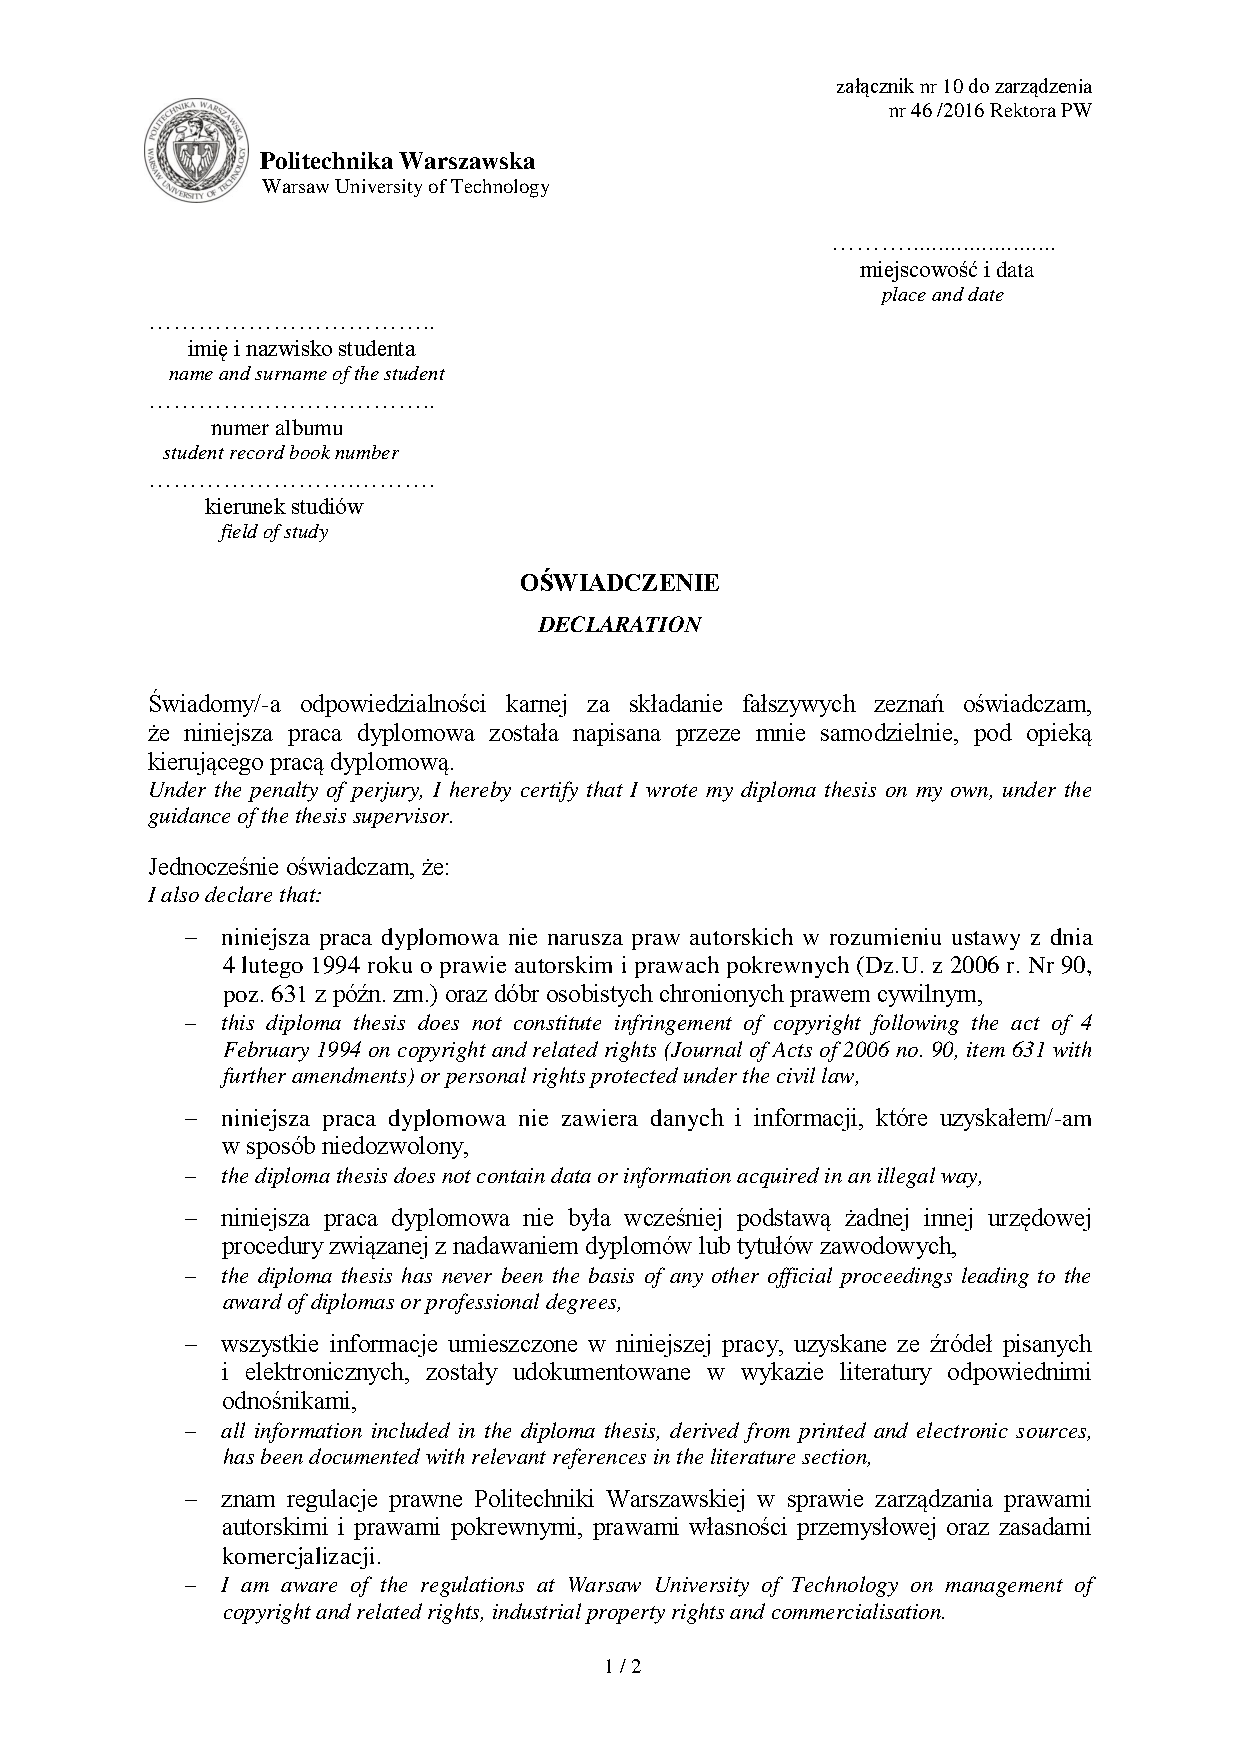
\includegraphics[width=\textwidth]{src/en/authorship/eiti-1.pdf}
\clearpage

\includegraphics[width=\textwidth]{src/en/authorship/eiti-2.pdf}

% \pagestyle{plain}
%--------------
% Spis treści
%--------------
\cleardoublepage % Zaczynamy od nieparzystej strony
\tableofcontents

%------------
% Rozdziały
%------------
\cleardoublepage % Zaczynamy od nieparzystej strony
\pagestyle{headings}
\section{Introduction}

The field of mobile robots is expanding quickly and has the potential to completely transform a variety of industries. Mobile robots are becoming increasingly common in our daily lives as the need for automation rises. These robots are capable of assisting from healthcare to industrial automation. The advent of autonomous vehicles has revolutionized the transportation industry, promising safer and more efficient travel. However, the realization of this vision hinges on the development of advanced technologies capable of enabling these vehicles to navigate their environment safely and efficiently. One such technology is real-time object recognition, which allows autonomous vehicles to identify and classify objects in their path. 

Autonomous vehicles rely heavily on sensors and computer vision algorithms to perceive their surroundings. These systems must be able to process large amounts of data in real time to make quick decisions, often within milliseconds. The challenge lies in developing algorithms that can accurately recognize objects while maintaining high computational efficiency.  Obstacle avoidance, which is essential for autonomous navigation, is one of the major problems in mobile robots. In the realm of mobile robotics, obstacle avoidance stands as a fundamental challenge, empowering robots to traverse cluttered environments with both safety and efficiency \cite{wenzel2021vision}.\\
 Traditional obstacle avoidance methods, such as sonar, laser scanning, and stereo vision, have served as the cornerstone of these systems. However, these methods have inherent limitations, particularly in terms of their ability to handle dynamic and unpredictable scenarios.

Recently, the integration of deep learning, a subset of machine learning, has brought about a paradigm shift in the field of autonomous vehicles. Deep learning algorithms, particularly Convolutional Neural Networks (CNNs), have proven to be highly effective in tasks such as image and speech recognition, natural language processing, and beyond 2. In the context of autonomous vehicles, deep learning has been instrumental in enhancing the perception of surroundings, driver behavior monitoring, path planning, sensor fusion, and intelligent control of vehicle dynamics 1.

Deep learning-based control algorithms are especially crucial for achieving full autonomy. They can manage complex lateral and longitudinal maneuverings and can effectively calculate steering commands for lateral control and acceleration and braking commands for longitudinal speed control of vehicle 1. However, the safety of deep neural networks can be unstable under adverse conditions, necessitating the use of varied datasets for training the automated control system 1.

This paper is focused on the application of deep learning in real-time object recognition for autonomous vehicles. 







\section{Problem Statement}
Developing real-time object detection systems for obstacle avoidance represents a nuanced and intricate task, necessitating meticulous consideration. The efficacy of such systems is contingent upon several pivotal factors, encompassing the quality of visual data, the intricacies of the underlying algorithms, and the overall architecture of the obstacle avoidance system. A thorough exploration of each of these components is imperative to optimize the system for superior performance.

In addressing this inquiry, a comprehensive examination of the influencing factors is undertaken, seeking avenues for their refinement and enhancement. The goal is to engineer an obstacle-avoidance system of the highest quality. Furthermore, it is essential to contemplate the broader implications of the obstacle avoidance solution, assessing how it contributes to heightened safety and enhanced mobility across diverse contexts. By prioritizing these fundamental aspects, a profound understanding of the challenges inherent in real-time object detection systems can be cultivated. This nuanced understanding serves as a foundation for the development of innovative solutions, leveraging advanced computer vision techniques to surmount these obstacles.

\section{General Objective:}
The general objective of this study is to develop a deep learning-based obstacle avoidance system for mobile robots using Neural Architecture Search(NAS) in Python. The aim is to enable mobile robots to perceive their environment, detect obstacles in real time, and navigate safely through complex surroundings in real time.
\subsection{Specific Objectives:}

\begin{itemize}
     \item Collect and curate a dataset of labeled images for training the obstacle detection neural network.
    \item Preprocess the dataset by applying techniques such as image augmentation and normalization to improve the network's performance.
    \item Design and implement a neural network architecture suitable for obstacle detection and avoidance.
    \item Train the neural network using the COCO dataset, optimizing the network's parameters and hyperparameters.
    \item 	Integrate the trained neural network into the mobile robot's control system for real-time obstacle detection and avoidance
    \item Evaluate the performance of the obstacle avoidance system using quantitative metrics such as accuracy, precision, recall, and F1 score.
    \item Compare the neural network-based approach with traditional methods of obstacle avoidance in terms of effectiveness, efficiency, and adaptability.
    \item Assess the robustness and generalization capabilities of the trained neural network by testing it in various environments and with different types of obstacles.
    \item Identify potential areas for further improvement and research in computer vision-based obstacle avoidance, such as multi-sensor fusion or incorporating depth information.
    \item Provide practical insights and recommendations for implementing computer vision-based obstacle avoidance systems for mobile robots using neural networks in Python.
\end{itemize}

\section{General Theory}
\subsection{Image processing}
Image processing is a method of performing operations on an image to extract information or enhance its features. It is a broad field that covers a range of techniques, including image acquisition, Pre-processing, segmentation, feature extraction, image analysis, and visualization. In general, image processing involves transforming an image into a more useful form for analysis or display. This can be achieved through a variety of techniques, such as filtering, edge detection, Thresholding, and morphological operations. Image processing has numerous applications in various fields, including medicine, remote sensing, surveillance, robotics, and entertainment. \cite{wilhelm2016digital}, \cite{tyagi2018understanding} 

\subsection{Deep Learning and Neural Networks}
Deep learning is another name for a multilayer artificial neural network or multilayer perceptron. The elementary
bricks of deep learning are the neural networks, that are combined to form the deep neural networks.

\begin{table}[htbp]
\centering
\caption{Comparing Neural Networks and Deep Learning}
\footnotesize
\begin{tabular}{ |p{3cm}|p{5cm}|p{5cm}| }%{ |c|c|c| }
\hline
Feature & Neural Networks & Deep Learning \\
\hline
Structure & Single-layer or shallow neural networks (typically two to three layers) & Deep neural networks with multiple layers (typically more than three) \\
\hline
Learning Ability & Can learn simple patterns and make predictions & Can learn complex patterns, including abstract relationships, and make more accurate predictions \\
\hline
Data Requirements & Requires less training data & Requires more training data to learn complex patterns patterns \\
\hline
Computational Cost & Less computationally expensive & More computationally expensive, especially for deep neural networks with many layers \\
\hline
Applications & Image classification, fraud detection, spam filtering & Image recognition, natural language processing, speech recognition, medical diagnosis, self-driving cars \\
\hline
\end{tabular}
\end{table}

The term "deep" in deep learning refers to the use of multiple layers in the neural network. Deep learning models, often called deep neural networks (DNNs), are capable of learning and representing complex patterns and hierarchical features from data. \cite{nielsen2015neural} \cite{Arnold2011AnIT}, \cite{2015Natur.521..436L} \\

Various types of deep learning systems exist, distinguished by their neural network architectures and operational principles. Examples include feed-forward neural networks, convolutional networks, recurrent neural networks, autoencoders, and deep beliefs. These methodologies have facilitated substantial advancements in sound and image processing domains, encompassing tasks such as facial recognition, speech recognition, computer vision, automated language processing, and text classification (e.g., spam detection). The potential applications of these techniques are diverse. An illustrative instance is the AlphaGo program, which achieved world champion status in the game of Go in 2016 by leveraging deep learning methodologies.\cite{koons2005}, \cite{shinde2018review}, \cite{choi2020introduction}
\begin{figure}[H]
    \centering
    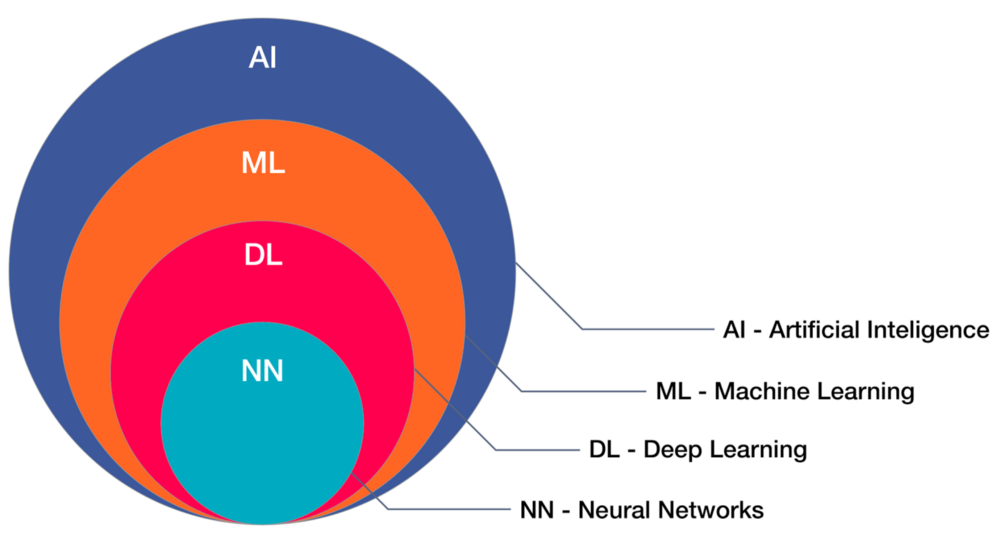
\includegraphics[width=0.8\linewidth]{tex/img/NN_DL_ML.png}
    \caption{Neural network core of deep learning \cite{an}}
    \label{fig:NN_DL}
\end{figure}

\subsection{Neural Networks}
Neural networks are the fundamental components of deep learning. They are composed of layers of interconnected nodes or neurons that process information.
Artificial neural networks (ANNs) are computing systems that are designed to work in a similar way to the human brain.

\subsubsection{The Biological Inspiration}
The complexity of the brain has made it challenging for scientists to fully understand it, despite extensive research. Engineers have modified neural models to create a more useful and less biological approach, while still maintaining much of the original terminology.
\begin{figure}[H]
    \centering 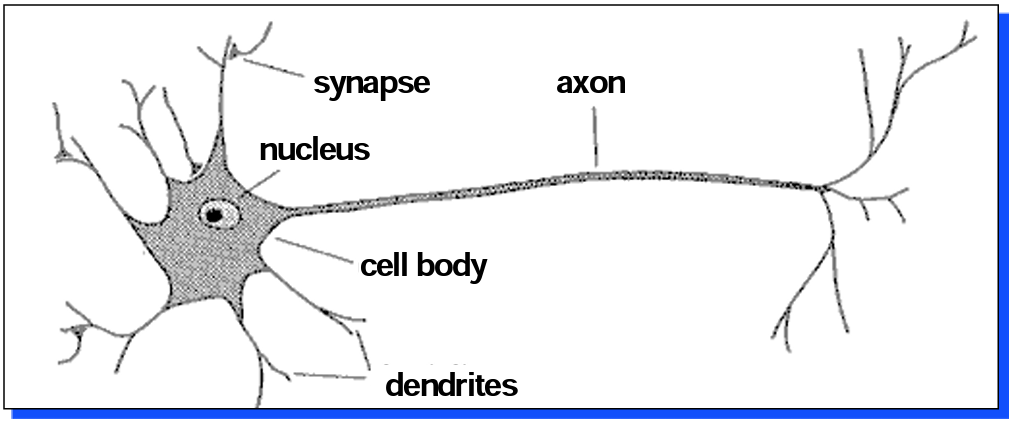
\includegraphics[width=0.5\linewidth]{tex/img/Structure_of_Neurons.PNG}
    \caption{The structure of Neurons \cite{nielsen2015neural}}
    \label{fig:Neuron structure}
\end{figure}
A neuron is composed of three main parts - the cell body, the dendrite (which branches out to receive input), and the axon (which branches out to send output). Connections between axons and dendrites are made via synapses. Electro-chemical signals are carried from the dendrites, through the cell body, and down the axon to other neurons.


\subsubsection{Perceptron}
A single neuron of a neural network is called a perceptron. A perceptron implements a mathematical function that operates on the input signals and generates outputs. Figure is an example of a perceptron. A perceptron is the simplest neural network.
\subsubsection{The learning process}
A perceptron model starts by multiplying all the input values and their weights and then sums these values to create a weighted sum. This weighted sum is then applied to the activation function "f" to obtain the desired result. This activation function is also known as a step function and is represented by "f". This step function or activation function plays an essential role in ensuring that the output signal is mapped between the required values (0,1) or (-1,1). Please note that the weight of the input data indicates the strength of the node. similarly, the value of the input bias allows the activation function curve to shift up or down.
The input signals to a neuron come either from a source (a camera or sensing device) or from the outputs of other neurons.

\begin{figure}[H]
    \centering
    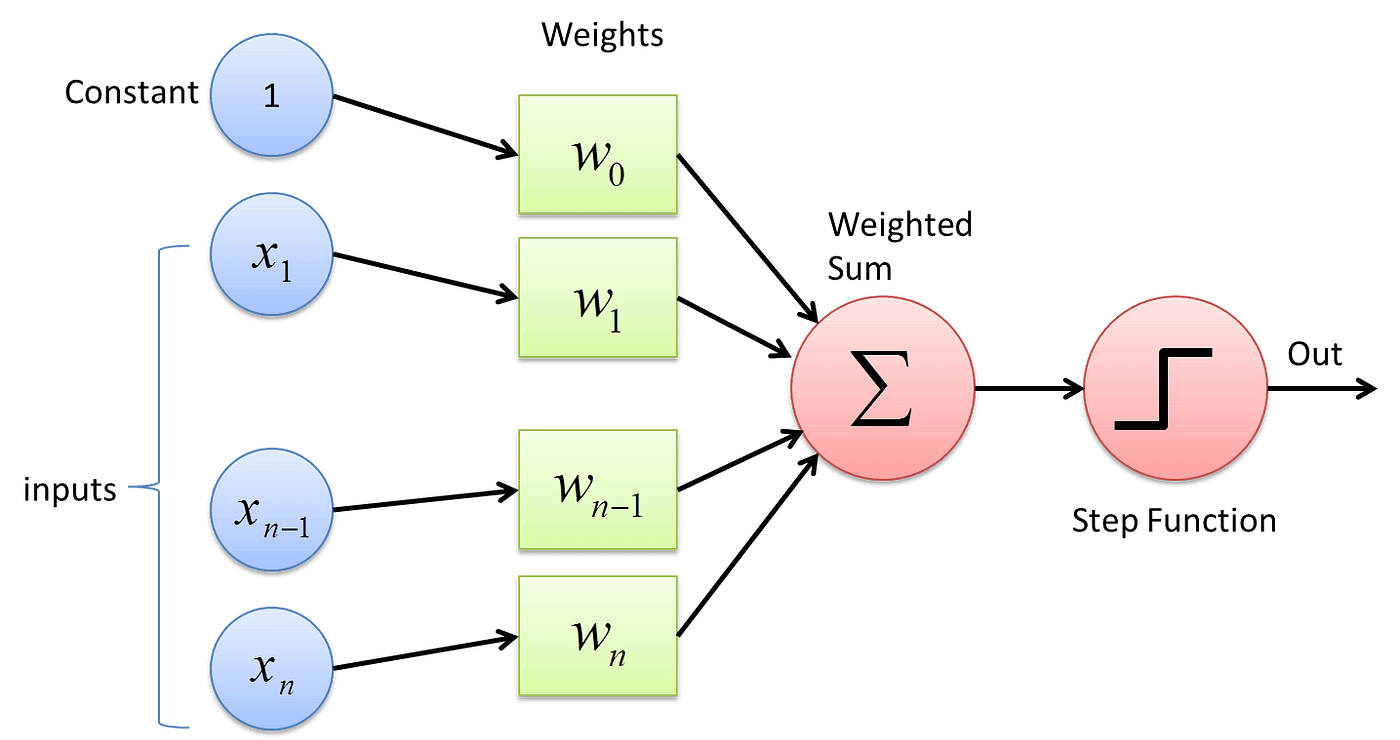
\includegraphics[width=0.7\linewidth]{tex/img/Perceptron.png}
    \caption{Perceptron}
    \label{fig:Perceptron}
\end{figure}

Mathematically, the output (y) of a neuron in a neural network perceptron can be expressed as:\\

\(y=f(\sum_{i=1}^{n}(\omega_{i}.x_{i})+b)\)

where:\\
$\omega_{i}$ is the weight associated with the input \(x_{i}\)\\
\(b\) is the bias term,\\
\(f:\) activation\\
As shown in fig \ref{fig:Perceptron}, One percepteron has the following components: \\
\begin{itemize}
    \item \textbf{Input Nodes or Input Layer: }  
    The input layer, also called input nodes, is the first layer of a neural network. It is responsible for receiving input data, which can be any numerical values, images or text. The input layer does not perform any calculations or transformations of the input data, but only forwards them to subsequent layers in the network. \cite{ansari2020building}, \cite{nielsen2015neural}\\
    \item \textbf{Weight: } Weights are parameters that adjust the strength of the connections between neurons (nodes) in adjacent layers of a neural network. Each connection has an associated weight, and these weights are learnable and updated during the training process. The weights determine the impact of the input signals on the neurons in the next layer. A higher weight means that the corresponding input has a stronger influence on the neuron's output. During training, the neural network adjusts these weights to minimize the difference between the predicted output and the actual target output. \\
    \item \textbf{Bias: } Biases are additional parameters in a neural network that allow for fine-tuning the output of each neuron. Unlike weights, biases are not associated with specific inputs but are added to the weighted sum of inputs in each neuron.
    Role: Biases provide the neural network with flexibility, enabling it to account for situations where all inputs are zero or have low values. They allow neurons to activate even when the weighted sum of inputs is not sufficient to trigger an output.Like weights, biases are adjusted during training to improve the overall performance of the network. \cite{ansari2020building}, \cite{nielsen2015neural}\\
    \item \textbf{Activation Function: } The primary purpose of an activation function is to determine whether a neuron should be activated (output a signal) or not, based on the input it receives.
    An activation function is a mathematical operation enacted on the output of a neuron (or node) within the architecture of a neural network. It introduces non-linearity to the network, allowing it to learn complex patterns and make more sophisticated decisions. The activation function takes the weighted sum of inputs and a bias term and produces the output of the neuron.\cite{nielsen2015neural}

\end{itemize}
\subsubsection{Types of Perceptron: }
Based on the layers, Perceptron models are divided into two types.
\begin{enumerate}
    \item \textbf{Single-layer perceptron model:}  This is one of the simplest types of artificial neural networks (ANN). The single-layer perceptron model consists of a feedforward network and also includes a threshold transfer function inside the model. The main goal of the single-layer perceptron model is to analyze linearly separated objects with binary outputs.

    In a single-layer perceptron model, its algorithms do not contain recorded data, so it starts with a non-constantly allocated input for weight parameters. Furthermore, it sums all inputs (weight). If, after adding all inputs, the sum of all inputs is greater than the set value, the model will be activated and display the output value as +1.
    If the result is the same as the previously established threshold value, then the performance of this model is considered satisfactory and the weight requirements do not change. However, this model contains several discrepancies that arise when many input weight values are introduced into the model. Therefore, some changes should be necessary when entering the weights to find the desired result and minimize errors.
    A single-layer perceptron learns patterns that can be solved linearly. \cite{ansari2020building}, \cite{knerr1990single}

        \item \textbf{Multi-layer Perceptron} An artificial neural network, similar to the human brain, comprises several neurons, also known as perceptrons. A cluster of neurons processes the inputs. Every individual neuron within the group separately processes the inputs. The outputs from this cluster of neurons are transmitted to another individual neuron or cluster of neurons for subsequent processing. These neurons can be visualized as organized in layers, where the output of one layer serves as the input for the following layer. There is no limit to the number of layers you can use to train your neural network. The arrangement of neurons in a neural network, where multiple layers are used, is referred to as a multilayer perceptron (MLP). A multi-layer perceptron model shares the same structure as a single-layer perceptron model, but it includes a higher number of hidden layers.
    \begin{figure}[H]
        \centering
        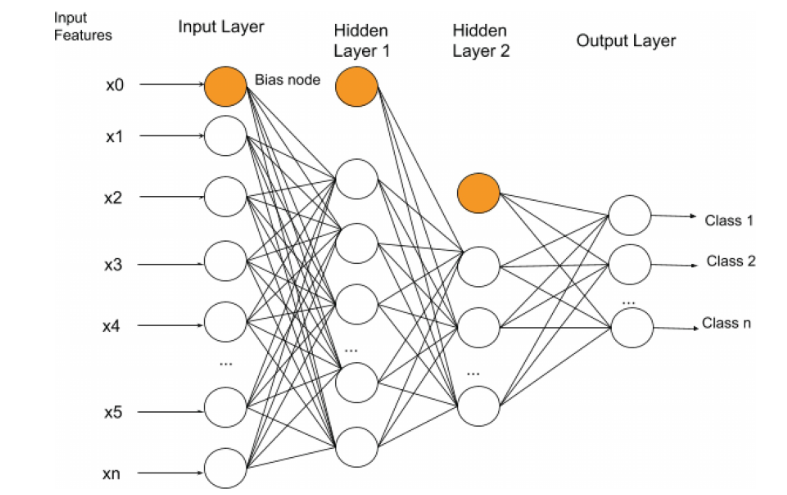
\includegraphics[width=0.8\linewidth]{tex/img/MLP.PNG}
        \caption{Multi layer perceptron \cite{ansari2020building}}
        \label{fig:MLP}
    \end{figure}
also known as the backpropagation algorithm, which executes in two stages as follows:
    \begin{itemize}
        \item \textbf{Forward Stage:} Activation functions start from the input layer in the forward stage and terminate at the output layer.
        \item \textbf{Backward Stage:} In the backward stage, weight and bias values are modified as per the model's requirements. In this stage, the error between the actual output and demand originates at the output layer and propagates backward to the input layer.
    \end{itemize}
A multi-layer perceptron model is a type of artificial neural network that has greater processing power and is capable of processing both linear and non-linear patterns. It is also capable of implementing logic gates such as AND, OR, XOR, NAND, NOT, XNOR, and NOR.

This model has multiple artificial neural networks with several layers, where the activation function is not linear as in a single-layer perceptron model. Instead, it can be executed with various activation functions such as sigmoid, TanH, ReLU, etc., for deployment. \cite{ansari2020building}, \cite{nielsen2015neural}
\end{enumerate}

\subsection{Deep Learning}
Deep learning is a type of artificial neural network or multilayer perceptron. It is a subset of machine learning that focuses on using artificial neural networks and representational learning. The term "deep" in deep learning refers to the use of multiple layers in the network. These methods can be supervised, semi-supervised, or unsupervised. \cite{vargas2017deep}

Various deep-learning architectures, such as deep neural networks, deep belief networks, deep reinforcement learning, recurrent neural networks, convolutional neural networks, and transformers, have been successfully applied to several fields, including computer vision, voice recognition, signal processing, natural language processing (NLP), machine translation, bio-informatics, drug or medical purposes, climate forecasting, material inspection, and board game programs. These architectures have produced remarkable results that are comparable to, and in some cases, surpassing human expert performance. \cite{hosseini2020deep}

\subsubsection{Deep Learning or Multilayer Perceptron Architecture}
A multilayer perceptron consists of at least three types of layers: the input layer, the hidden layers, and the output layer. You can have more than one hidden layer. Each layer contains one or more neurons. A neuron performs some computation on the inputs it gets and generates outputs. The output from the neurons is sent as input to the next layer, except in the case of the output layer.

\begin{enumerate}
    \item \textbf{Input layer: } This is the primary component of Perceptron, which accepts the initial data into the system for further processing. Every input node in the system holds a numerical value that is real and can be expressed as a number.
In a neural network, the input layer receives raw input data like image, text, etc. It then passes it on to the next layer. Each node in the input layer represents a feature or an attribute of the input data. These nodes act as receptors for the raw input information and are connected to the nodes in the next layer, which is typically a hidden layer.
    
Here are some key points about the input layer:
    \begin{enumerate}
\item Nodes/Neurons: The nodes in the input layer are also called input neurons. Each neuron corresponds to a specific feature or dimension of the input data.
\item Input Features: If you're working with a dataset of, for example, images, each node in the input layer might represent a pixel's intensity or color values. In the case of text data, each node could represent a unique word or a character.
\item No Processing: The nodes in the input layer do not perform any processing on the input data. They simply pass the raw input values to the next layer. The actual computation and learning occur in the subsequent layers, particularly in the hidden layers.
\item Connections: Each node in the input layer is connected to every node in the next layer (usually a hidden layer) through weights. These weights determine the strength of the connection between nodes and play a crucial role in the learning process of the neural network.
    \end{enumerate}
    The input layer of a neural network consists of neurons that are equal in number to the features of the data. Along with these neurons, additional nodes called bias nodes can also be included in each layer. The primary purpose of the bias node is to provide control over the output of the layer. Although not strictly necessary in deep learning, it is still a common practice to add a bias node.
    
    \textbf{Total Number of Neurons in the input layer} = The number of input features without a bias = (The number of input features + 1) with a bias 
    \cite{ansari2020building}\\
    \item \textbf{Hidden Layers: } Hidden layers in a neural network refer to the layers that come between the input layer and the output layer. They are called "hidden" because their outputs are not directly observable or part of the final network output during the training phase. At least one hidden layer is necessary for a neural network to function as this is where the learning occurs. The neurons in this layer perform the computations required for learning. Generally, for most cases, a single hidden layer is sufficient for learning. However, as required to model real-world situations, the number of hidden layers can be increased. As the number of hidden layers increases, the computation complexity of the network also increases, which leads to an increase in computation time.
    \\
    
    \textbf{Total Number of Neurons in the hidden layer} = A common practice is to take two-thirds (or 66 percent) of the number of neurons in the previous layer.\\
    
    For example, if the number of neurons in the input layer is 100, the number of neurons in the first hidden layer will be 66 and in the next hidden layer will be 43, and so on. Again, there is no magic number, and you should tune the neuron counts based on the model accuracy.
    \item \textbf{Output Layer: } The output layer is the final layer in a neural network, responsible for producing the model's predictions or outputs based on the learned representations from the preceding layers. The number of neurons in the output layer depends on the problem type that the neural network is supposed to solve. \\
    \textbf{Nodes in the Output Layer can be used for:}
    \begin{itemize}
        \item \textbf{For binary classification: } there is typically one node with a sigmoid activation function, producing a probability output.\\
        \item \textbf{For multi-class classification: } when the network has to predict one of many classes, the output layer has as many neurons as the number of all possible classes.\\
        \item \textbf{For regression tasks: } there is usually a single node with a linear activation function, producing a continuous output/ when the network has to predict a continuous value, such as the closing price of stocks, the output node has only one neuron. \cite{calin2020deep}, \cite{nielsen2015neural}
    \end{itemize}
\end{enumerate}
\subsubsection{Forward propagation}

A feedforward neural network is a type of artificial neural network comprising neurons interconnected in a manner that avoids cyclic connections. This architecture represents the most basic form of the neural network, where data propagation occurs unidirectionally, from the input layer through the hidden layer(s), and ultimately to the output layer. Unlike its counterparts, this network lacks any loopback or feedback mechanism, enabling a linear flow of information through its layers. \cite{coates2011analysis} \cite{ansari2020building} 
\begin{figure}[H]
    \centering
    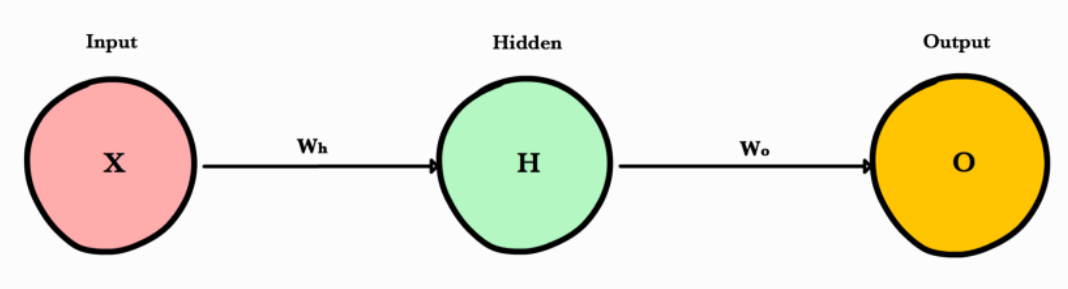
\includegraphics[width=0.7\linewidth]{tex/img/Forwardpropagation.PNG}
    \caption{Forward Propagation \cite{ajitjaokar}}
    \label{fig:enter-label}
\end{figure}
a single pass of forward propagation translates mathematically to:
\[Prediction=A(A(XW_{h})W_{o})\]
Where A:    is an activation function like ReLU, X is the input and $W_{h}$ and $W_{o}$ are weights.\\

\textbf{Steps}\\
- Calculate the weighted input to the hidden layer by multiplying X by the hidden weight $W_{h}$.\\
- Apply the activation function and pass the result to the final layer \\
- Repeat step 2 except this time X is replaced by the hidden layer’s output, H \cite{ansari2020building}, \cite{nielsen2015neural}

\subsubsection{BackPropagation: }
The main objective of back propagation is to modify or adjust the weights in the neural network in a way that corresponds to their contribution to the overall error. By consistently reducing the error associated with each weight, we can eventually obtain a set of weights that generate accurate predictions. \\
Here are the final 3 equations that together form the foundation of backpropagation. \cite{hecht1992theory} \cite{nielsen2015neural}
 \[
 Output Layer Error    E_{o} = (O-y).R'(Z_{o})
 \]
 \[ 
 Hidden Layer Error    E_{h} = E_{o}.W_{o}.R'(Z_{h})
 \]
 \[ 
 Cost-Weights Deriv \hspace{3mm}   LayerError.LayerInputs
 \]


\begin{figure}[H]
    \centering
    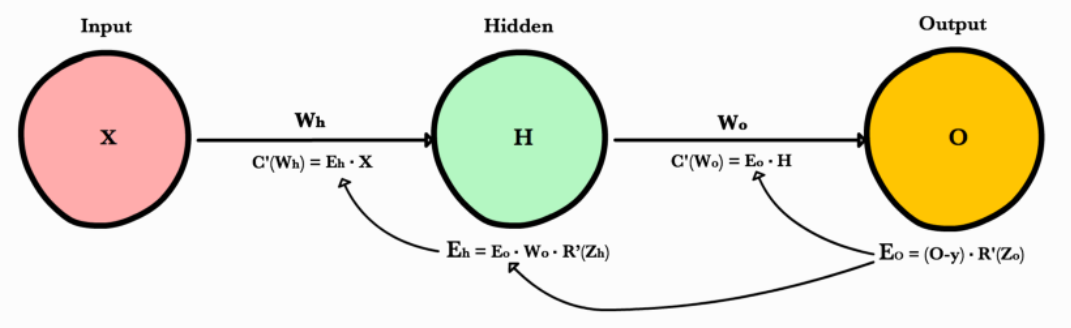
\includegraphics[width=0.8\linewidth]{tex/img/backward_propagation.PNG}
    \caption{Backward Propagation \cite{ajitjaokar}}
    \label{fig:backward_propagation}
\end{figure}
\subsubsection{Activation function}
The activation function plays a crucial role in determining whether a neuron should be activated (turned on or off) based on whether its input is relevant for model prediction. This function normalizes the output of each neuron to a range between 0 and 1 or between -1 and 1. Different mathematical functions are utilized as activation functions for various purposes.\cite{sharma2017activation}, \cite{apicella2021survey}, \cite{bfortuner_mlglossary}

we can broadly divide the activation function into two: \\
\begin{itemize}
    \item \textbf{Linear Activation Function: } Commonly used in the output layer for regression tasks where a continuous range of values is desired. A linear activation function computes a weighted sum of its input without introducing non-linearity, and The output is a linear transformation of the input. 
    \begin{figure}[H]
        \centering
        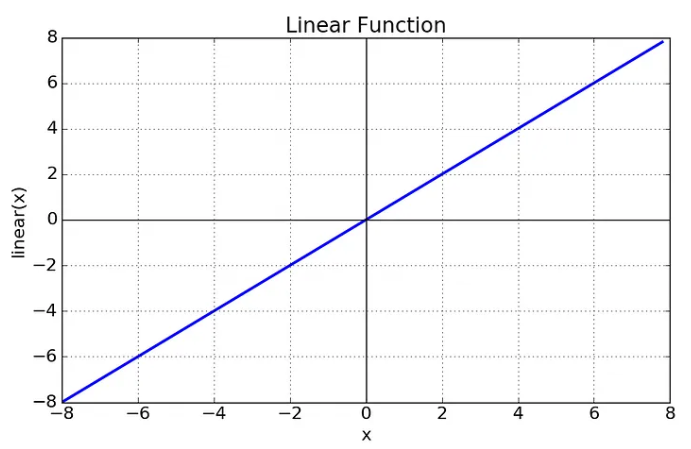
\includegraphics[width=0.5\linewidth]{tex/img/Linear_function.PNG}
        \caption{Linear Activation Function}
        \label{fig:LAF}
    \end{figure}
    \textbf{Equation: }
    \(f(x)=cx\) \\where c is constant.\\
    
    The output of the linear activation function varies from $-\infty$ to  $+\infty$, as shown in Figure above.
     If you choose to use a linear activation function, the last layer of your neural network will simply be a linear function of the first layer, regardless of how many layers the network has. This means that your network can only learn linear dependencies between the input and output, which is insufficient for solving complex problems like computer vision. Therefore, using a linear activation function is not recommended for such problems. \cite{bfortuner_mlglossary}\\
     \item \textbf{Non-linear Activation Function: } A non-linear activation function introduces non-linearity into the network, enabling it to learn complex relationships and representations. It facilitates the model's ability to generalize and differentiate outputs with diverse data.
    \begin{figure}[H]
        \centering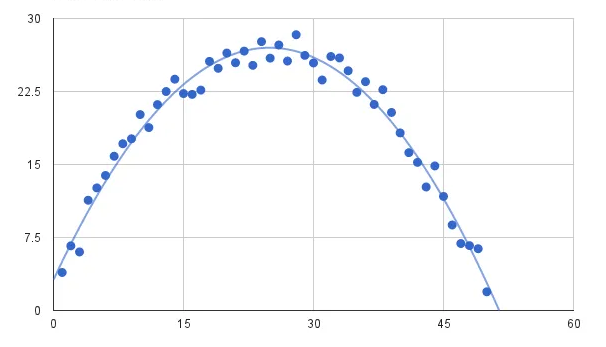
\includegraphics[width=0.5\textwidth]{Non-Linear.PNG}
        \caption{Non-Linear Activation Function}
    \end{figure}
    Essential for training deep neural networks as it allows the network to capture complex patterns and relationships in the data, They allow the network to capture intricate relationships between features, which is crucial for tasks like image recognition, natural language processing, and more.
    \begin{enumerate}
        \item \textbf{Sigmoid or Logistic Activation Function: } 
    The sigmoid activation function calculates the neuron output using the sigmoid function, as shown here:
    $$\phi(z)=\frac{1}{1+e^{-z}}$$
    \begin{figure}[H]
        \centering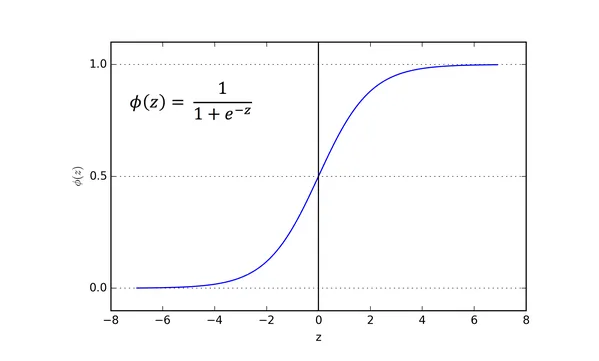
\includegraphics[width=0.5\textwidth]{sigmoid_Activation.PNG}
        \caption{Sigmoid Activation Functioin}
    \end{figure}
    where \(z\) is calculated like \\
    
    $$z=X_0+\sum_{i=0}^{i=n}w_{i}x_{i}$$
    
    The sigmoid function is a mathematical operation that always yields a value between 0 and 1. This makes the output spontaneous, without many overrides as the input value fluctuates. Additionally, the sigmoid function is very useful as it does not generate a constant value from the first-order derivatives because it is a non-linear function.
    
    The sigmoid function is a mathematical function that always produces an output value between 0 and 1. This characteristic results in a smooth output without many jumps as the input value fluctuates. Another benefit of the sigmoid function is that it is nonlinear, and its first-order derivative does not generate a constant value.
    \item \textbf{Tanh or hyperbolic tangent Activation Function}
    
    The Tanh function is a type of activation function, commonly used in neural networks. Its behavior is similar to the sigmoid activation function, but with some notable differences. The Tanh function is zero-centered, and The range of the tanh function is from (-1 to 1).
    
    \begin{figure}[H]
        \centering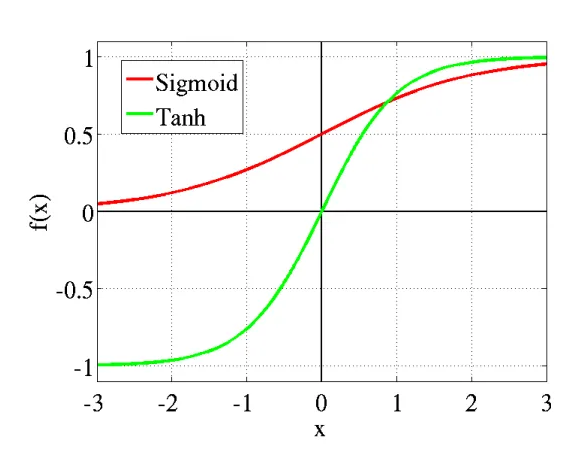
\includegraphics[width=0.5\textwidth]{Tangent_activation.PNG}
        \caption{Tangent Activation Functioin}
    \end{figure}
    
    The TanH activation function calculates the neuron output using:\\
    $$tanh(z)=\frac{e^{z}-e^{-z}}{e^{z}+e^{-z}}$$
    The TanH is useful when it comes to mapping the values; the negative inputs will be mapped strongly to negative, and the same for positive inputs too, and the zero inputs will be mapped near zero.
    \item \textbf{ReLU (Rectified Linear Unit) Activation Function}
   The Rectified Linear Unit (ReLU) is a widely used activation function in deep learning, particularly for computer vision tasks. ReLU is preferred for image processing because it can handle non-negative values, which is a common characteristic of image pixels. One of the key advantages of ReLU is its computational efficiency, which makes it suitable for large-scale models. Furthermore, ReLU is a nonlinear function with a derivative, allowing for backpropagation and weight adjustment during training. This property is essential for the neural network to learn from the data and improve its performance over time.
    
    \begin{figure}[H]
        \centering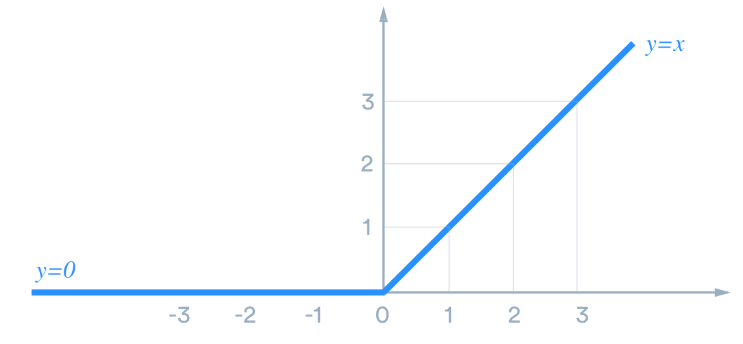
\includegraphics[width=0.5\textwidth]{Relu_Activation.PNG}
        \caption{ReLU Activation Functioin}
    \end{figure}
    
    
    $$f(x)=max(0,x)$$
    it ranges from 0 to +$\infty$\\
    \item  \textbf{Leaky ReLU Activation Function}
    The leaky rectified linear unit (ReLU) is a widely used activation function in deep learning models. The function introduces a small negative slope in the negative region, which allows for backpropagation for negative inputs, thereby avoiding the vanishing gradient problem. However, a drawback of this function is that it produces inconsistent outputs for negative values. This is because the negative slope of the activation function results in a non-zero output for negative inputs, which is not consistent with the expected behavior of an activation function. Nonetheless, the leaky ReLU remains a popular choice for deep neural networks due to its ability to improve the training of deep models.
    \begin{figure}[H]
        \centering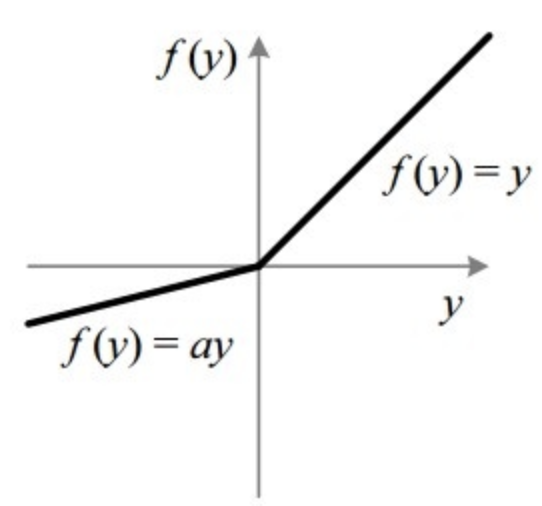
\includegraphics[width=0.5\textwidth]{leaky_relu.png}
        \caption{Leaky ReLU Activation Functioin}
    \end{figure}
    
    $f(y)=\left\{\begin{array}{rcl}
         \alpha y & \mbox{for} & y<0\\
         y & \mbox{for} & y\geq 0
    \end{array}\right.$\\
    \item \textbf{SELU Actiovation Function}
    A scaled exponential linear unit (SELU) computes neuron outputs using the following equation:
    
    $f(\alpha,x)=\lambda\left\{\begin{array}{rcl}
         \alpha (e^{x}-1) & \mbox{for} & x<0\\
          x & \mbox{for} & x\geq 0
    \end{array}\right.$\\
    \\
    where the value of $\lambda$ = 1.05070098 and the value of $\alpha$ = 1.67326324. These values are fixed and do not change during backpropagation.[Orielly]
    \begin{figure}[H]
        \centering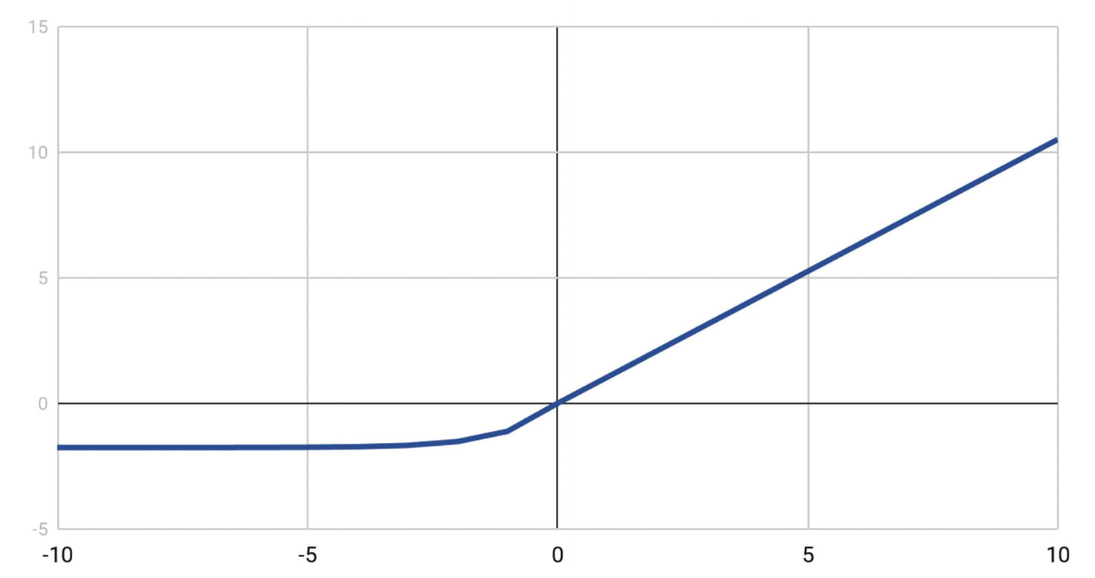
\includegraphics[width=0.5\textwidth]{SELU_activation.PNG}
        \caption{SELU Activation Functioin}
    \end{figure}
    
   SELU is an activation function that has the property of self-normalization. This means that with SELU, the entire network is self-normalizing, which makes it efficient in terms of computation and helps it converge faster. Additionally, SELU overcomes the issues of exploding or vanishing gradients that occur when the input features are too high or too low.
    \item \textbf{Softplus Activation Function}
    The softplus activation function applies smoothing to the activation function value 
    \(z\) . It uses the log of exponent as follows:\\
    
    $$f(x)=lon(1+e^{z})$$\\
    \\
    Softplus is also called the SmoothReLU function. The first derivation of the softplus function is  $\frac{1}{1+e^{z}}$, which is the same as the sigmoid activation function. 
    
    \begin{figure}[H]
        \centering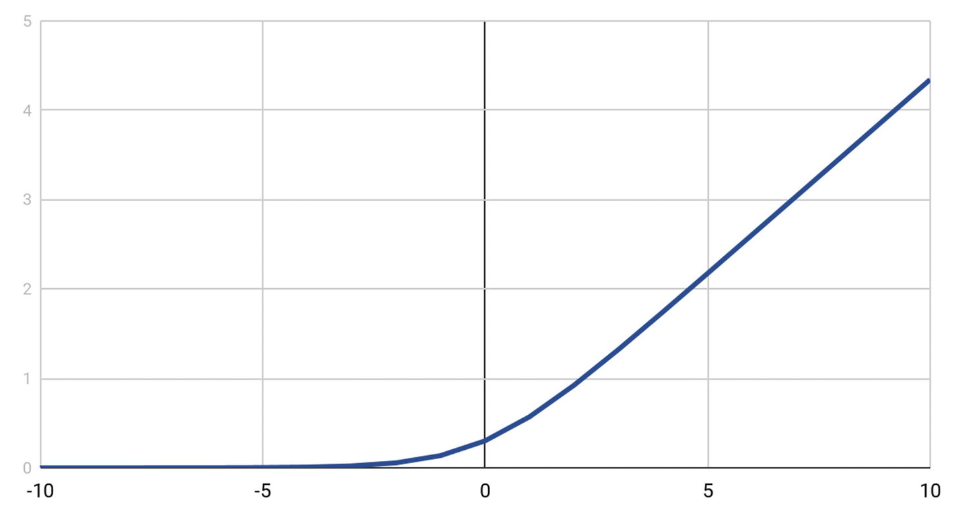
\includegraphics[width=0.5\textwidth]{Softplus_activation.PNG}
        \caption{Softplus Activation Function}
    \end{figure}
    \item \textbf{Softmax}
    The Softmax function operates on a vector of real numbers by normalizing it to create a probability distribution that generates outputs between 0 and 1. The resulting probabilities have the property that the sum of all output values is equal to 1. This function is typically utilized as the activation function for the output layer of a classification neural network. The interpreted output values represent prediction probabilities for each class.
    \begin{figure}[H]
        \centering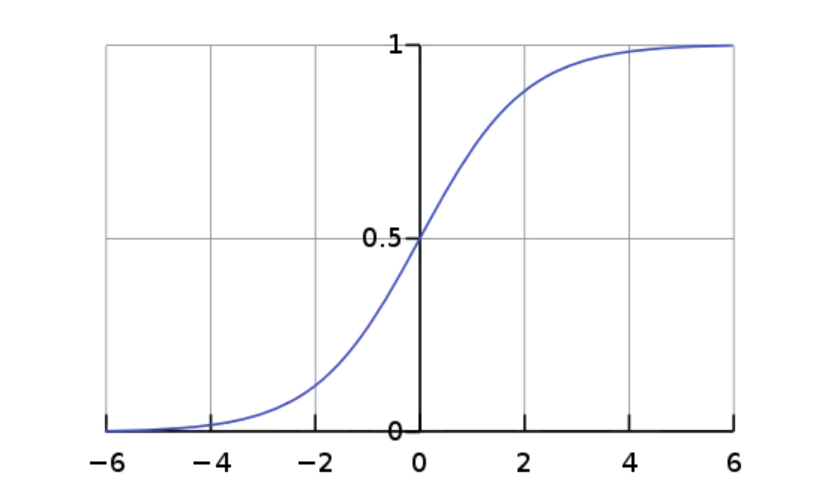
\includegraphics[width=0.5\textwidth]{Softmax.PNG}
        \caption{Softmax Activation Function}
    \end{figure}
    $$\sigma(z)_{i}=\frac{e^{z_{i}}}{\sum_{j=1}^{k}e^{z_{j}}}$$ for \(i\)=1,...., k and z=$(z_{1}....,z_{k})$ $\epsilon R^{k}$
    \end{enumerate}
\end{itemize}

\subsubsection{Loss Function/Error Function}
A loss function is a function that measures how well a neural network models the training data by comparing the target and predicted output values. During training, the goal is to minimize the loss between the predicted and target outputs.
The equation of error may be written in a simplified form as follows:\\

\(Error = Expected outcome - Predicted outcome\)\\

When a neural network begins the learning process, it initializes weights and calculates output from each neuron using an activation function. It then computes the error, adjusts the weights, recalculates outputs, and re-evaluates errors, until it reaches the minimum error. The weights that give the minimum errors are considered the final weights and the network is considered "learned" at this stage.

In calculus, if the first derivative of a function is zero, then the function at that point is either a minimum or a maximum. The neural network training process aims to find the minimum point where the first derivative is zero. To achieve this, a neural network must have an \textbf{error function} that calculates the first derivative and identifies the points (weights and biases) where the error function is minimum. The type of error function used depends on the type of model being trained. These error functions are also called loss functions or simply losses.\\

The error functions are broadly divided into the following three categories: \cite{ansari2020building}, \cite{heaton2018ian}\\
\begin{itemize}
    \item \textbf{Regression loss functions} are used when we want to train models to predict continuous value outcomes, typically a numerical value. To measure the difference between the predicted and actual target values, different loss functions are employed. The following are some widely used regression loss functions:\\
    \begin{itemize}
    \item \textbf{Mean Squared Error (MSE) Loss:} This is the default error function for regression problems. This is the preferred loss function if the distribution of the target variable is normal or Gaussian. This function has numerous properties that make it especially suited for calculating loss. The difference is squared, which means it does not matter whether the predicted value is above or below the target value; however, values with a large error are penalized.\\
    $$MSE=\frac{1}{n}\sum_{i=1}^{n}(y^{(i)}-\hat{y}^{(i)})^{2}$$
    \item  \textbf{Mean Absolute Error (MAE) Loss:}  MAE finds the average of the absolute differences between the target and the predicted outputs.
    $$MAE=\frac{1}{n}\sum_{i=1}^{n}|y^{(i)}-\hat{y}^{(i)}|$$
    In some cases, this loss function serves as an alternative to MSE. As mentioned earlier, MSE is highly sensitive to outliers, which can significantly affect the loss due to the squared distance. To mitigate this, MAE is used when the training data has a substantial number of outliers.
    \item \textbf{The Mean Squared Logarithmic Error (MSLE)} The Mean Squared Logarithmic Error (MSLE) is a loss function that is commonly used in regression tasks. It is particularly useful when the target values span multiple orders of magnitude. MSLE measures the mean squared difference between the natural logarithm of the predicted values and the natural logarithm of the true values. This can be especially helpful when there is a wide variation in the scale of the target values.
    The formula for MSLE is as follows:
     $$MSLE(y,\hat{y})=\frac{1}{n}\sum_{i=1}^{n}(log(1+y^{(i))}-log(1+\hat{y}^{(i)}))^{2}$$
     where: \\
     $y^{i}: $ is the true target value for the \(i\)-th sample.\\
     $\hat{y}^{(i)}: $ is the predicted target value for the \(i\)-th sample.
     \item \textbf{Huber Loss: } The Huber loss, also referred to as the smooth L1 loss, is a commonly used loss function in regression tasks. It is designed to be less sensitive to outliers compared to the Mean Squared Error (MSE) loss function while retaining the benefits of a quadratic loss function for smaller errors.

     $$Huber(y,\hat{y})=\frac{1}{n}\sum_{i=1}^{n}L_{\delta}(y^{(i))}-\hat{y}^{(i)})$$
     where: \\
     $y_{i}: $ is the true target value for the \(i\)-th sample.\\
      $y^{i}: $ is the predicted target value for the \(i\)-th sample.\\
      $n: $ is the total number of samples.\\
      $L_{\delta}(x)$ is defined as:
      
      $L_{\delta}(x)=\left\{\begin{array}{rcl}
           \frac{1}{2}x^{2} & \mbox{for} & |x| \leq \delta \\
          \delta(|x|-\frac{1}{2}\delta) & otherwise 
      \end{array}\right.$\\
      \textbf{Benefit: } One big When training neural networks, using Mean Absolute Error (MAE) can cause a problem due to its large gradient, which can result in missing the minima at the end of training when using gradient descent. In contrast, as the loss gets closer to its minima, the gradient decreases when using Mean Squared Error (MSE), making it more accurate.
    
    To address this issue, Huber loss can be very useful since it curves around the minima, decreasing the gradient. Additionally, Huber loss is more resistant to outliers than MSE. Therefore, it combines the desirable properties of both MSE and MAE.
    \item  \textbf{Log-Cosh loss: } The Log-Cosh loss is a smooth and differentiable approximation of the Huber loss, often used in regression tasks. Similar to the Huber loss, it aims to be less sensitive to outliers than the Mean Squared Error (MSE) loss, but it has the advantage of being continuously differentiable.
     $$Log-Cosh(y,\hat{y})=\frac{1}{n}\sum_{i=1}^{n}Log(cosh(y^{(i))}-\hat{y}^{(i)}))$$
     where: \\
      $y_{i}: $ is the true target value for the \(i\)-th sample.\\
      $y^{i}: $ is the predicted target value for the \(i\)-th sample.\\
      $n: $ is the total number of samples.\\
      \(Cosh: \) is the hyperbolic cosine function.\\
      The optimization goal during training is to minimize the Log-Cosh loss, and the model adjusts its parameters to achieve predictions that result in smaller Log-Cosh loss values. The Log-Cosh loss is often considered when a balance between the robustness of the Huber loss and the differentiability of the MSE loss is desired.
      \item \textbf{Quantile loss function: } Quantile loss is a loss function used in quantile regression, where the goal is to predict not just a central tendency (like the mean in traditional regression) but rather different quantiles of the target distribution. It is particularly useful when you want to estimate a range of possible values for a prediction.
      $$L_{\gamma}(y, y^{p})=\sum_{i=y_{i}<y_{i}^{p}}(\gamma-1).|y_{i}-{y_{i}^{p}}|+ \sum_{i=y_{i}\geq y_{i}^{p}}(\gamma).|y_{i}-y_{i}^{p}|$$

      The optimization goal during training is to minimize the Quantile Loss, and the model adjusts its parameters to achieve predictions that capture the desired quantiles of the target distribution. Quantile regression is particularly useful in scenarios where understanding the variability or uncertainty in predictions is essential.
      
    
     
    \end{itemize}
    \item \textbf{Binary classification loss functions} are used when we want to train models to predict a maximum of two classes (usually denoted as 0 and 1) and the true binary label, such as to compare and contrast different classes together. \\
          \begin{itemize}
          \item \textbf{Binary Crossentropy Loss (Log Loss): } The Binary Crossentropy Loss (Log Loss) is the default loss function for binary classification problems and is considered better than other functions. It calculates a score that reflects the average difference between the actual and predicted probability distributions for predicting class 1. This score is minimized, and a perfect cross-entropy value is set to 0. The function can only be used when the target value is within the range of (0,1).
          $$Binary Crossentropy(y, \hat{y})=\frac{1}{n}\sum_{i=1}^{n}[y_{i}log(\hat{y_{i}})+(1-y_{i})log(1-\hat{y_{i}})]$$

          It measures the cross-entropy between the true binary labels and the predicted probabilities. It penalizes deviations from the true labels by assigning higher penalties to confidently wrong predictions.
          \item \textbf{Hinge Loss (SVM Loss):} This is used mainly in support of vector machine–based binary classification and can be used when the target variable is in the range (-1, 1).
          $$Hinge-Loss(y,\hat{y})= \frac{1}{n}\sum_{i=1}^{n}max(0,1-y_{i}.\hat{y_{i}})$$

          Penalizes misclassifications linearly and encourages correct predictions to have a margin of at least 1.

          \item \textbf{Squared Hinge Loss: } The squared hinge loss function computes the squared value of the score hinge loss. This mathematical operation smooths the surface of the error function, rendering it numerically more tractable.
          \[
          \text{Squared Hinge Loss}(y,\hat{y})=\frac{1}{n}\sum_{i=1}^{n}max(0,1-y_{i}.\hat{y_{i}})^{2}
          \]
      \end{itemize}
    \item \textbf{Multiclass classification loss functions} are used when our models need to predict more than two classes/are used to measure the difference between predicted class probabilities and true class labels in scenarios where there are more than two classes, such as object detection. \\
          \begin{itemize}
          \item \textbf{Categorical Crossentropy Loss: } used for multiclass classification tasks with one-hot encoded true class labels. It is used to measure the cross-entropy between the true distribution and the predicted class probabilities.
          $$Categorical Crossentropy(y,\hat{y_{i}})=-\frac{1}{n}\sum_{i=1}^{n}\sum_{j=1}^{m}y_{ij}log(\hat{y_{ij}})$$
          \item \textbf{Sparse Categorical Crossentropy Loss: } Similar to categorical crossentropy but used when true class labels are provided as integers rather than one-hot encoded vectors.
          $$Sparse Categorical Crossentropy(y,\hat{y})=-\frac{1}{n}\sum_{i=1}^{n}log(\hat{y_{i}[y_{i}]})$$
          Sparse cross-entropy performs the same cross-entropy calculation of error without requiring that the target variable be one hot-encoded before training and is used When you have a large number of classes in the target, for example, predicting dictionary words.
          \item \textbf{Kullback-Leibler divergence (KLD) loss: }The Kullback-Leibler divergence (KLD) loss is a measure of the dissimilarity between one probability distribution and a reference baseline distribution. A value of 0 for the KL divergence loss indicates that both distributions are identical. This statistical metric quantifies the amount of information loss, expressed in bits, when the predicted probability distribution is employed to approximate the target probability distribution.

        The KLD loss is a valuable tool for addressing complex problems, such as auto-encoders, which are utilized for learning high-dimensional representations. In the context of multiclass classification, KLD serves as a multiclass cross-entropy measure.
        \[
        \text{KL Divergence}(P \parallel Q) = \sum_{i \in \chi} P(i) \log\left(\frac{P(i)}{Q(i)}\right)
        \]
        where:\\
        For discrete probability distributions, P and Q are defined on the same sample space, $\chi$, the relative entropy from Q to P.
        \item \textbf{Cross-Entropy Loss (Sigmoid Crossentropy for Multilabel Classification): }
        Suitable for multilabel classification where each sample can belong to multiple classes. It measures the crossentropy for each class independently.

         \[
         \text{Cross Entropy Loss}(y,\hat{y})=-\frac{1}{n}\sum_{i=1}^{n}[y_{i}log(\sigma(\hat{y_{i}}))+(1-y_{i})log(1-\sigma(\hat{y_{i}}))]
         \]
      \end{itemize}

\end{itemize}

\subsubsection{Layers}
In a neural network, layers are the building blocks that organize and structure the computation. Each layer contains a group of nodes, or neurons, that process information.
\begin{itemize}
    \item \textbf{Convolutional Layer: } In convolutional neural networks (CNN), the convolution layer performs a linear operation by multiplying the input with a weight (kernel or filter), and it plays a critical role in the network. The layer comprises two primary components: \\
    \begin{itemize}
        \item \textbf{Kernel (Filter): } A convolution layer can comprise more than one filter. The size of the filter should be smaller than the input dimension intentionally, as it allows the filter to be applied at different positions on the input. Filters are useful for identifying significant features in a given input. By applying more than one filter to the same input, different features can be extracted. The output from multiplying the filter with the input creates a dimensional array called the "feature map."

        The Stride property controls the movement of the filter over the input. When the value is set to 1, the filter moves one column at a time over the input. When set to 2, the filter jumps two columns at a time as it moves over the input.
    \end{itemize}
    \item \textbf{Dropout Layer: } A dropout layer is a type of layer commonly used in neural networks to prevent overfitting. It takes the output of the previous layer's activations and randomly sets a certain fraction, known as the dropout rate, of the activations to 0. This effectively cancels or "drops out" those activations, helping to prevent the network from becoming too reliant on any one feature or pattern. The dropout rate is a tunable hyperparameter that can be adjusted to measure performance with different values. Typically, it is set between 0.2 and 0.5, but it can be set arbitrarily depending on the specific application and dataset.
    
    Dropout is a technique used during training of neural networks. During training, some of the activations in a layer are randomly dropped or turned off. However, at test time, no activations are dropped, instead, they are scaled down by a factor of the dropout rate. This is to account for the fact that more units are active during test time than during training time. The idea behind dropout is to introduce some noise into the layer in order to disrupt any interdependent learning or coincidental patterns that may occur between units in the layer that are not significant. This helps to prevent overfitting and improve the generalization performance of the network. \\
    \item \textbf{Pooling layer: }Pooling layers often take convolution layers as input. A complicated dataset with many objects will require a large number of filters, each responsible for finding patterns in an image so the dimensionally of a convolutional layer can get large. It will cause an increase in parameters, which can lead to over-fitting. Pooling layers are a type of technique that is used to reduce the dimensionality of high-dimensional data. Similar to convolutional layers, pooling layers also have a kernel size and stride. The kernel size is typically smaller than the feature map, with a standard size of 2x2 and a stride of 2. There are two main types of pooling layers that are commonly used.

    The first type is the max pooling layer. The Max pooling layer will take a stack of feature maps (convolution layer) as input. The value of each node in the max pooling layer is calculated by taking the maximum value of the pixels contained in a sliding window. This operation helps to reduce the size of the feature maps while preserving the most important information.
    
    The other type of pooling layer is the: \\
    \textbf{Average Pooling layer}. The average pooling layer calculates the average of pixels contained in the window. It's not used often but you may see this used in applications for which smoothing an image is preferable.\\
    \item \textbf{Fully-connected/Linear Layer: } A fully-connected layer, also called a linear layer, is a type of layer in a neural network where all the inputs from one layer are connected to every activation unit of the next layer. Usually, the last few layers in machine learning models are fully-connected ones, which output a class prediction based on the features learned in the previous layers.

To input a vector of nodes activated in the previous convolutional layers, the fully-connected layer passes it through one or more dense layers before sending it to the output layer. An activation function is used to make a prediction before the vector reaches the output layer. While the convolutional and pooling layers tend to use a ReLU function, the fully-connected layer can use two activation functions depending on the classification problem:

- Sigmoid:  is a mathematical function that is commonly used for binary classification problems. It is a logistic function that has a characteristic "S" shaped curve.
- Softmax: A more generalized logistic activation function that ensures the values in the output layer sum up to 1. It is commonly used for multi-class classification.

The activation function outputs a vector with the same dimensions as the number of classes to be predicted. The output vector yields a probability between 1 and 0 for each class. \cite{schmidhuber2015deep}, \cite{goodfellow2016deep}\\
   
\subsubsection{Optimizer}
An optimizer is an algorithm or method used to adjust the parameters of the neural network (weights and biases) during the training process. The primary goal of an optimizer is to minimize the loss function, which measures the difference between the predicted output and the true target values.

During training, the neural network makes predictions, and the optimizer adjusts the model's parameters based on the error (loss) between these predictions and the actual target values. The optimization process involves finding the optimal set of parameters that minimize the loss, enabling the neural network to make accurate predictions on unseen data. \cite{choi2019empirical}, \cite{ansari2020building} 

Some commonly used optimizers in neural networks include:
\begin{itemize}
    \item \textbf{Adaptive gradient (Adagrad): } Adaptive gradient (Adagrad) is a technique that adjusts the learning rate according to a specific parameter. 
\begin{itemize}
    \item This method ensures that parameters with higher gradients or frequent updates have a slower learning rate, so as not to overshoot the minimum value.
    \item parameters with low gradients or infrequent updates have a faster learning rate, allowing them to be trained quickly.
    \item  It divides the learning rate by the sum of squares of all previous gradients of the parameter.
    \item When the sum of the squared past gradients has a high value, it basically divides the learning rate by a high value, so the learning rate will become less.
    \item Similarly, if the sum of the squared past gradients has a low value, it divides the learning rate by a lower value, so the learning rate value will become high.
    \item This implies that the learning rate is inversely proportional to the sum of the squares of all the previous gradients of the parameter.
    \end{itemize}
    \[
    g_{t}^{i}=\frac{\partial J(w_{t}^{i})}{\partial \mathbf{W}}
    \]
    \[
    \mathbf{W}=\mathbf{W}-\alpha\frac{\partial J(\omega_{t}^{t})}{\sqrt{\sum_{r=1}^{t}(g_{r}^{i})^2+\epsilon}}
    \]
    where: \\
     $g_{t}^{i}$  the gradient of a parameter\\
    $\alpha$ : the learning rate\\
    $\epsilon: $ very small value to avoid dividing by zero
    
    \item \textbf{Adaptive delta(Adadelta): } Adadelta is a type of stochastic gradient descent algorithm that offers adaptive techniques for hyperparameter tuning. The name Adadelta is derived from "adaptive delta", where delta refers to the difference between the current weight and the newly updated weight.

    Adadelta is an improved version of Adagrad that adjusts learning rates based on a moving window of gradient updates, instead of accumulating all past gradients. This allows Adadelta to continue learning even after many updates have been made.
    
    The update rule in Adadelta eliminates the need to set a default learning rate, making it unnecessary to specify a learning rate.
    
    \[
    v_{t}=\rho v_{t-1}+(1-\rho)\bigtriangledown_{\theta}^{2}J(\theta)
    \]
    \[
    \bigtriangleup\theta=\frac{\sqrt{\omega_{t}+\epsilon}}{\sqrt{v_{t}+\epsilon}}\bigtriangledown_{\theta}J(\theta)
    \]
    \[
    \theta=\theta-\eta\bigtriangleup\theta
    \]
    $\omega_{t}=\rho\omega_{t-1} + (1-\rho)\bigtriangleup\theta^{2}$
    \item \textbf{Adam Optimizer: } The Adam optimizer combines concepts from both RMSProp and Momentum to help in computing adaptive learning rates for each parameter. It works as follows:
    \begin{itemize}
        \item Firstly, it computes the exponentially weighted average of past gradients $(v_{dW})$
        \item  Secondly, it calculates the exponentially weighted average of the squares of past gradients $(s_{dW})$
        \item Thirdly, to counteract any bias towards zero, a bias correction is applied to these averages  $(v_{dW}^{corrected}, s_{dW}^{corrected})$
        \item Lastly, the parameters are updated using the information from the calculated averages\\
        \[v_{dW}=\beta_{1}v_{dW}+(1-\beta_{1})\frac{\partial J}{\partial W}\]
        \[
        s_{dW}=\beta_{2}s_{dW}+(1-\beta_{2}) \left(\frac{\partial J}{\partial W}\right)^{2}
        \]
        \[
         v_{dW}^{corrected}=\frac{v_{dW}}{1-(\beta_{1})^{t}}
        \]
        \[
         s_{dW}^{corrected}=\frac{s_{dW}}{1-(\beta_{1})^{t}}
        \]
        \[
        W=W-\alpha\frac{v_{dW}^{corrected}}{\sqrt{s_{dW}^{corrected}} + \epsilon}
        \]
        where:\\
        $v_{dW}$-  the exponentially weighted average of past gradients\\
        $s_{dW}$- the exponentially weighted average of past squares of gradients\\
        $\beta_{1}$- hyperparameter to be tuned\\
        $\beta_{2}$- hyperparameter to be tuned\\
        $\frac{\partial J}{\partial W}$ - cost gradient with respect to current layer\\
        W- the weight matrix (parameter to be updated)\\
        $\alpha$ - the learning rate\\
        $\epsilon$ - very small value to avoid dividing by zero\\
    \end{itemize}
    \item \textbf{RMSProp Optimizer: } RMSProp optimizer is an adaptive learning rate optimization algorithm that helps to speed up convergence. It does this by keeping an exponentially weighted average of past gradient squares and dividing the learning rate by this average. This process results in a more efficient and faster convergence of the algorithm.
    \[
    s_{dW} = \beta s_{dW} + (1-\beta)\left(\frac{\partial J}{\partial W}\right)^{2}
    \]
    \[
    W = W-\alpha\frac{\frac{\partial J}{\partial W}}{\sqrt{s_{dW}^{corrected}}+ \epsilon}
    \]
    
    where: \\
    s - the exponentially weighted average of past squares of gradients\\
    $\frac{\partial J}{\partial W}$-  cost gradient with respect to current layer weight tensor\\
    W - weight tensor\\
    $\beta$- hyperparameter to be tuned\\
    $\alpha$- the learning rate\\
    $\epsilon$- very small value to avoid dividing by zero.
    \item \textbf{Stochastic Gradient Descent(SGD) Optimizer: } Stochastic Gradient Descent (SGD) is a widely used optimization algorithm for training neural networks and other machine learning models. It is a variant of the gradient descent optimization algorithm that processes each training example individually rather than using the entire dataset in each iteration. This property makes it well-suited for large datasets. Optionally, partition the dataset into mini-batches of a fixed size.
    \begin{itemize}
        \item For each mini-batch or individual example:
        \item Compute the gradient of the loss with respect to the model parameters.
        \item Update the model parameters in the opposite direction of the gradient to minimize the loss.
    \end{itemize}.\\
    The update rule for the model parameters $\theta$ is given by:
    \[
    \theta_{t} = \theta_{t-1}-\alpha\bigtriangledown J(\theta_{t-1},x_{i}, y_{i})
    \]\\
    where: \\
    $\alpha : $  is the learning rate, a hyperparameter that controls the size of the steps taken during optimization.\\
    $\bigtriangledown J(\theta_{t-1},x_{i}, y_{i}$ is the gradient of the loss function $\mathbf{J}$ with respect to the parameters $\theta$ for the example $x_{i}, y_{i}$
\end{itemize}



\subsubsection{Regularization}
Regularization techniques are widely used in machine learning to reduce overfitting and improve the generalization performance of models. These methods introduce constraints or penalties to the training process, which encourage the model to be simpler and more robust. By doing so, they help to prevent the model from fitting too closely to the training data, thereby improving its ability to generalize to new, unseen data. \cite{goodfellow2016deep}, \cite{ansari2020building}, \cite{bishop2006pattern}
\begin{itemize}
    \item \textbf{Data Augmentation: }
    Having more data is the surest way to get better consistent estimators (ML model), in contrast having a small dataset will lead to the well-known problem of overfitting.
    Data augmentation refers to the technique of artificially increasing the size of a dataset by applying various transformations to the existing data. This is often used in deep learning, particularly in computer vision tasks, to improve the performance of neural networks.
    There are various types of data augmentation techniques, including:
    \begin{enumerate}
        \item  Flipping: horizontally or vertically flipping an image.
        \item Rotation: Rotating an image by a certain degree is the process of rotating the image based on a specific angle.
        \item Zooming: zooming in or out of an image.
        \item Translation: shifting an image horizontally or vertically.
        \item Cropping: cropping a portion of an image.
        \item Adding noise: adding random noise to an image.
        
    \end{enumerate}
    
    These techniques can be used individually or in combination to generate new data samples. By increasing the size of the dataset, the neural network is exposed to more variations of the same data, which helps improve its ability to generalize and make accurate predictions on new, unseen data. \cite{shorten2019survey}\\
    \item \textbf{Dropout: } is a technique used to reduce overfitting in neural networks. It works by randomly ignoring selected neurons during training, which prevents complex co-adaptations on the training data. 

    During the training process, some of the neurons are randomly dropped out, meaning that their contribution to the activation of downstream neurons is temporarily removed on the forward pass. Additionally, any weight updates are not applied to the neuron on the backward pass. 
    
    Simply put, the process of ignoring some of the neurons occurs during a particular forward or backward pass. The probability of randomly selecting nodes to be dropped out can be easily adjusted (e.g. 0.1\%) each weight update cycle.
    
    It is important to note that Dropout is only used during the training of a model and is not used when evaluating the model. \\
    \item \textbf{Early Stopping: } Early stopping is an alternative technique that can be used to prevent overfitting. This approach involves using the validation error to decide when to stop training the neural network.

    The biggest challenge in training a neural network is determining how long to train the model. If you train the model too little, it will result in underfitting in both the train and test sets. On the other hand, if you train it too much, it will overfit the training set and perform poorly on the test sets.
    
    The key is to train the network long enough that it can learn the mapping from inputs to outputs, but not so long that it overfits the training data. One possible solution is to treat the number of training epochs as a hyperparameter and train the model multiple times with different values. Then, you can select the number of epochs that results in the best accuracy on the train or a holdout test dataset.
    
    However, this solution requires training and discarding multiple models, which can be time-consuming and resource-intensive. \cite{goodfellow2016deep}\\
    \item \textbf{Ensembling: } Ensemble methods are machine-learning techniques that combine multiple models into one predictive model. There are two primary approaches to ensembling: Bagging and Boosting.:
    \begin{itemize}
        \item \textbf{Bagging} Bagging, which stands for bootstrap aggregation, is a technique that reduces the variance of an estimate by averaging multiple estimates. It involves training a large number of "strong" learners in parallel. A strong learner is a model that is relatively unconstrained. Bagging then combines all the strong learners to obtain a smoother and more accurate prediction.
        \item  \textbf{Boosting}
        Boosting is a family of algorithms that convert weak learners into strong learners. It involves a sequence of models, with each one focusing on learning from the mistakes of the previous model. The final result is a combination of all the weak learners, which results in a single strong learner.
        
        Bagging utilizes complex base models to “smooth out” their predictions, while boosting uses simple base models to "boost" their combined complexity.
    \end{itemize}
    Bagging uses complex base models and tries to “smooth out” their predictions, while boosting uses simple base models and tries to “boost” their aggregate complexity.\\
    \item \textbf{Injecting Noise: } Noise is a phenomenon commonly introduced to the inputs as a technique for dataset augmentation. In situations where the dataset is small, the neural network may tend to memorize the training dataset instead of learning the general mapping from the inputs to the outputs. In other words, the model may only memorize specific input examples and their respective outputs. To solve this problem and enhance the structure of the mapping, one approach is to add random noise to the inputs.

    By adding noise, the network becomes less prone to memorizing the training samples since they keep changing all the time. This leads to smaller network weights and a more robust network, which in turn results in lower generalization error.
    
    It's important to note that noise is only added during the training phase. No noise is added when the model is evaluated or used to make predictions on new data. Additionally, random noise can be added to other parts of the network during training. Some examples include:
    
    \begin{enumerate}
        \item \textbf{Noise Injection on Weights} Adding noise to the weights of a model can be seen as a form of regularization that encourages the model to not be overly sensitive to small changes in the weights. By doing so, the model is able to avoid finding only local minima and instead find global minima surrounded by flat regions. This can result in a more robust and accurate model.
        \item \textbf{Noise Injection on Outputs}  It is common for real-world datasets to have errors in their output labels. In order to address this issue, one approach is to explicitly model the noise in the labels. An example of this is the technique of Noise Injection on Outputs, which can be achieved through a process known as label smoothing.
    \end{enumerate}
    \item \textbf{L1 Regularization: } A regression model that uses the L1 regularization technique is called Lasso Regression. The objective of L1 regularization is to push some of the weight coefficients to zero, effectively performing feature selection. This results in a sparse model where only a subset of the input features are used. \cite{kukavcka2017regularization}

    The formula for L1 regularization is:\\
    Mathematically:\\
    
    \[
    \text{Loss}=\text{Error}(Y,\hat{Y})
    \]
    Following formula calculates the error With L1 Regularization function
    \[
    \text{Loss}=\text{Error}(Y-\hat{Y}) + \lambda\sum_{1}^{n}|\omega_{i}|
    \]
    
    where:\\
    \[
    \hat{Y}=\omega_{1} x_{1}+\omega_{2} x_{2}+...+\omega_{n}x_{n}+b
    \]
    L1 Regularization (or a variant of this concept) is a model of choice when the number of features is high Since it provides sparse solutions.\\
    
    \item \textbf{L2 Regularization: } L2 regularization is a technique used in regression models, and when it is applied, the model is called Ridge Regression. The primary difference between L1 and L2 regularization techniques is that L2 regularization adds a penalty term to the loss function, which is the squared magnitude of the coefficient. \cite{kukavcka2017regularization}

    Mathematical formula for L2 Regularization.
    \[
    \text{Loss}=\text{Error}(Y,\hat{Y})
    \]
    
    \[
    \text{Loss}=\text{Error}(Y-\hat{Y}) + \lambda\sum_{1}^{n}\omega_{i}^{2}
    \]
    
\end{itemize}

\subsubsection{Types of Deep learning architectures}

Deep learning architectures are neural network models that are specifically designed to learn and make predictions from complex datasets like images, speech, and text. There are a wide variety of algorithms and architectures used in deep learning to accomplish this task.
\begin{figure}[H]
    \centering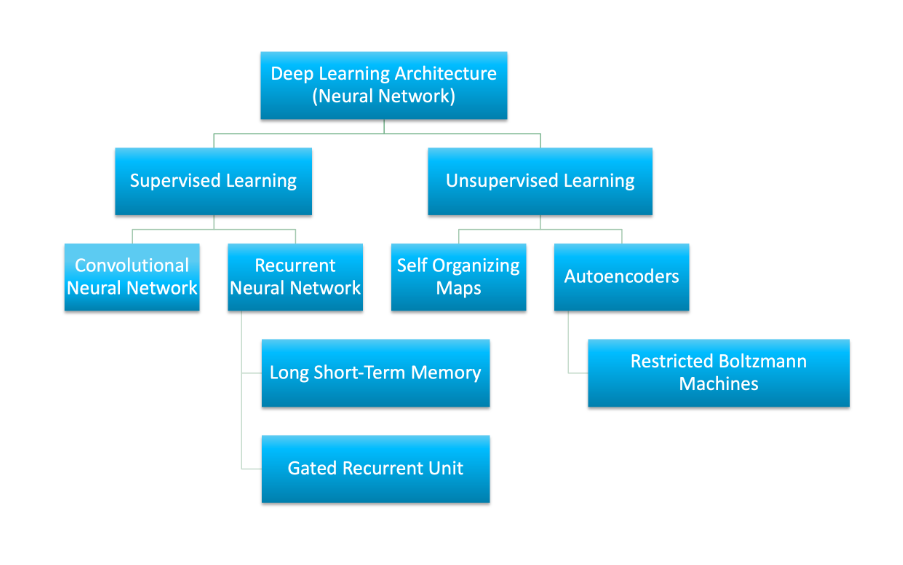
\includegraphics[width=1\textwidth]{DeepLearning_Arch.PNG}
    \caption{Deep learning architectures \cite{madhavan2017deep}}
\end{figure}
\begin{itemize}
    \item \textbf{Supervised deep learning: }
    Supervised learning refers to the problem space wherein the target to be predicted is clearly labeled within the data that is used for training.
    \begin{itemize}
        \item \textbf{Convolutional neural networks: } A CNN is a multilayer neural network used for image processing, inspired by the animal visual cortex. It was first created by Yann LeCun for recognizing handwritten characters. Early layers detect basic features, while subsequent layers combine these features to extract higher-level attributes of the input image. The LeNet CNN architecture performs feature extraction and classification through multiple layers, including convolutional and pooling layers, a fully connected multilayer perceptron, and an output layer. 
        \begin{figure}[H]
            \centering
            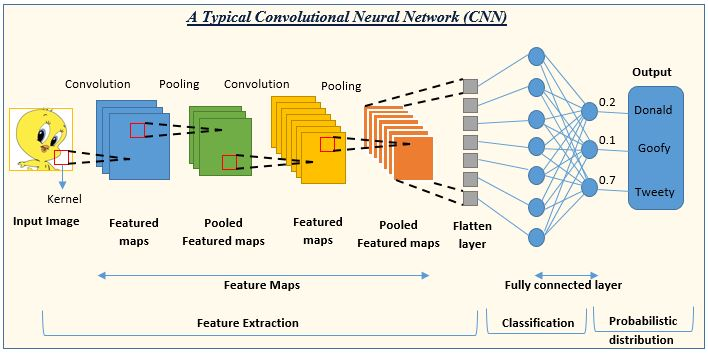
\includegraphics[width=0.8\linewidth]{tex/img/CNN.jpeg}
            \caption{Convolutional Neural Network \cite{Saily_Shah}}
            \label{fig:CNN}
        \end{figure}
        The network is trained through back-propagation. A Convolutional Neural Network (CNN) is a highly effective multilayer neural network that was inspired by the visual cortex of animals. It is primarily used for image processing applications. The first-ever CNN was created by Yann LeCun, which revolutionized the recognition of handwritten characters such as postal codes.
        
        With its deep network architecture, CNN can detect basic features, such as edges, through its initial layers and then combine these features to extract higher-level attributes of the input image.
        
        The LeNet CNN architecture, consisting of multiple layers that perform feature extraction and classification, is a prime example of CNN's effectiveness. It includes convolutional and pooling layers, a fully connected multilayer perceptron, and an output layer that identifies features of the image. The network is trained through back-propagation, making it an even more efficient tool. \cite{alzubaidi2021review} \cite{ansari2020building}
        
        \item  \textbf{The Gated Recurrent Unit (GRU) networks} In 2014, a simpler version of the LSTM network was introduced, known as the Gated Recurrent Unit (GRU). The GRU has two gates, an update gate and a reset gate, which replace the output gate present in the LSTM. The update gate determines how much of the previous cell contents should be kept, while the reset gate determines how to combine the new input with the previous cell contents. By setting the reset gate to 1 and the update gate to 0, a GRU can function as a standard RNN.\cite{madhavan2017deep}
        
        \begin{figure}[H]
            \centering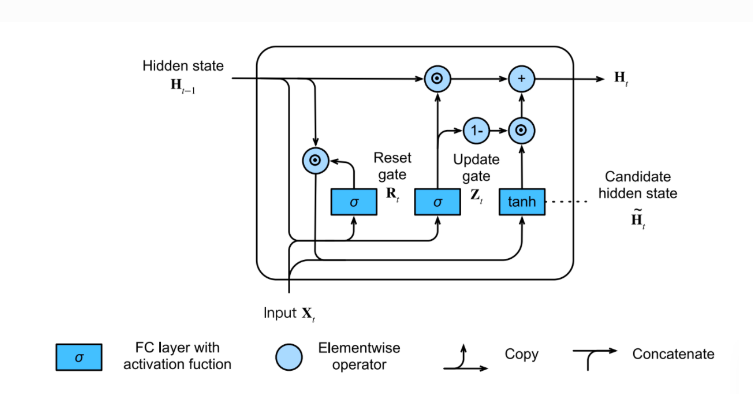
\includegraphics[width=1\textwidth]{GRU_layers.PNG}
            \caption{GRU networks \cite{bfortuner_mlglossary}}
        \end{figure}
        The LSTM is more expressive and can lead to better results with more data, while the GRU is simpler, can be trained more quickly, and can be more efficient in its execution.
    \end{itemize}

     \item \textbf{Recurrent Neural Network (RNN): } is a neural network that contains a hidden state which captures historical information up to the current timestep. The hidden state of the current state uses the same definition as the previous timestep, which makes the computation recurrent, hence its name.

    The RNN is a foundational network architecture from which other deep learning architectures are built. The primary difference between a typical multilayer network and an RNN is that an RNN may have connections that feed back into prior layers (or the same layer) instead of completely feed-forward connections. This feedback allows RNNs to retain memory of past inputs and model problems in time.
    
    RNNs include a rich set of architectures, and one popular topology is called Long Short-Term Memory (LSTM). The key differentiator is feedback within the network, which can appear from a hidden layer, the output layer, or some combination of both.
    
    RNNs can be unfolded over time and trained using standard backpropagation or a variant called backpropagation through time (BPTT).  \cite{sherstinsky2020fundamentals}\\
    \begin{figure}[H]
        \centering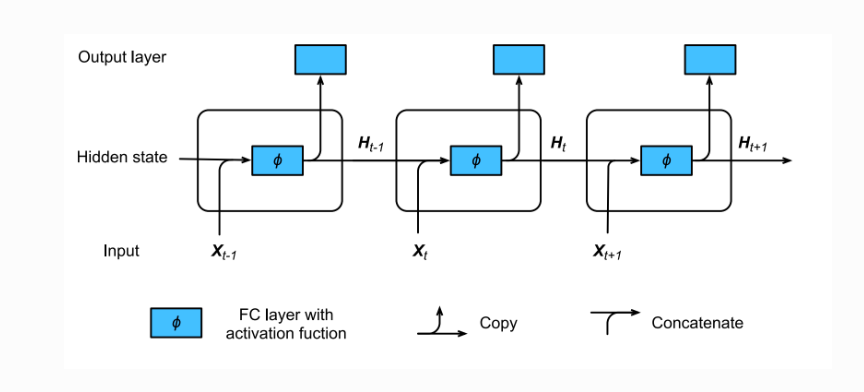
\includegraphics[width=0.8\textwidth]{RNN.PNG}
        \caption{Recurrent Neural Network \cite{bfortuner_mlglossary}}
    \end{figure}
    \item \textbf{Gated Recurrent Unit (GRU) Layer: } GRU supports: \\
    \textbf{hidden gate} the gating of hidden state, \\
    \textbf{Reset gate} controls how much of the previous hidden state we might still want to remember.\\
    \textbf{Update gate} controls how much of current hidden state is just a copy of the previous state
    The structure and math are as follow:
    \begin{figure}[H]
        \centering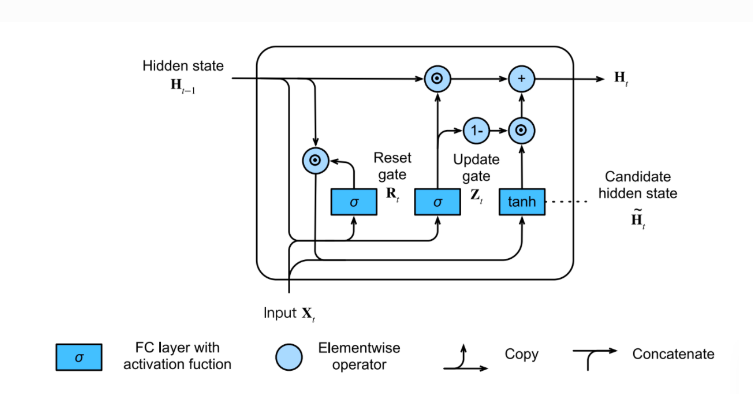
\includegraphics[width=0.8\textwidth]{GRU_layers.PNG}
        \caption{Gated Recurrent Unit \cite{bfortuner_mlglossary}}
    \end{figure}
    \item \textbf{Long short-term memory (LSTM): } Long Short-Term Memory (LSTM) is a type of recurrent neural network (RNN) architecture. It is specifically designed to address the vanishing gradient problem, which can occur in traditional RNNs. LSTMs are particularly useful for handling tasks that involve sequences of data, such as speech recognition, natural language processing, time series analysis, and more.

    The most remarkable feature of LSTMs is their ability to capture and remember long-term dependencies in sequential data while avoiding the vanishing gradient problem. This is a significant advantage over traditional RNNs, which can struggle with the training of long sequences. \cite{alzubaidi2021review} \cite{madhavan2017deep}
    
    Here are the main components and features of an LSTM:
    
    \textbf{Cell State (Ct):}
    
    The cell state in LSTM serves as a long-term memory. It remains unchanged throughout the chain of the LSTM network, with only some minor linear interactions. It works like a conveyor belt that runs through the entire sequence, and information can be added or removed from it as needed.\\
    
    \textbf{Hidden State (ht):}\\
    
    The hidden state in LSTM is essentially a short-term memory that plays a crucial role in capturing and retaining short-term dependencies in the sequence. It is determined by both the current input and the previous hidden state at each time step.\\
    \textbf{Input Gate: } 
    The input gate is responsible for determining the amount of newly received information that should be added to the cell state. It utilizes a sigmoid activation function to determine which values should be updated (values close to 1) and which values should be ignored (values close to 0).\\
    \textbf{Forget Gate: }
    The forget gate is responsible for determining which information from the cell state should be disregarded. It takes into account the previous hidden state and the current input to decide which parts of the cell state are no longer important. It utilizes a sigmoid activation function to produce output values ranging from 0 to 1.\\
    \textbf{Cell State Update: }
   Cell state update is determined by two gates - the input gate and the forget gate. These gates work together to decide what new information should be added to the cell state and what information should be removed from it. The input gate determines the new information to be stored, while the forget gate determines which information should be discarded.\\
    \textbf{Output Gate:}
    
    The output gate plays a crucial role in deciding the next hidden state. It utilizes two activation functions - sigmoid and tanh. Sigmoid determines which parts of the cell state should be outputted, while tanh generates a vector of new candidate values that are added to the hidden state.
    \href{https://ml-cheatsheet.readthedocs.io/en/latest/layers.html#lstm}{Layers}
    \begin{figure}[H]
        \centering
        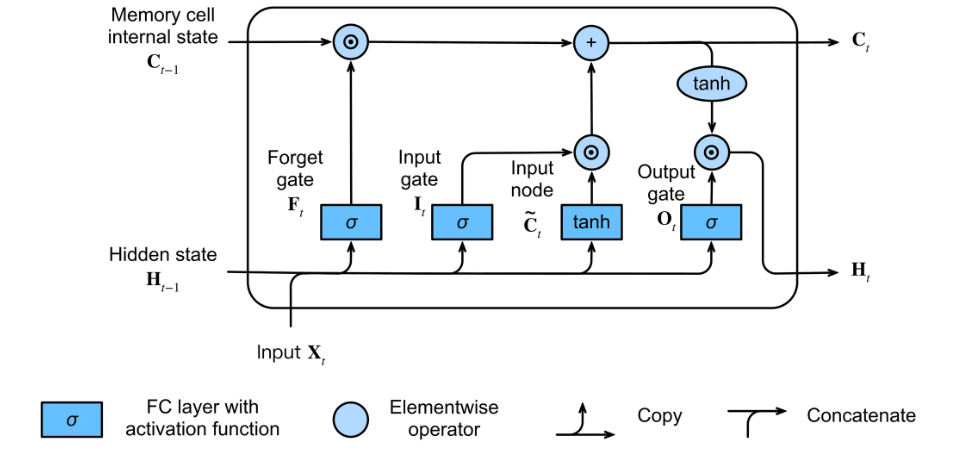
\includegraphics[width=0.8\linewidth]{tex/img/LSTM_layer.PNG}
        \caption{Long short-term memory \cite{yu2023popular}}
        \label{fig:LSTM_layer}
    \end{figure}
    \end{itemize}

\end{itemize}

\subsubsection{Section Unsupervised learning}

Unsupervised learning involves training models without target labels present within the data using unsupervised architectures.\cite{coates2011analysis}
\begin{itemize}
    \item \textbf{Self-organized maps: } Self-Organizing Maps (SOM) are a type of unsupervised neural network invented by Dr. Teuvo Kohonen in 1982, also known as Kohonen maps. Unlike traditional artificial neural networks, SOMs create clusters of input data by reducing input dimensionality. \cite{alzubaidi2021review}, \cite{madhavan2017deep}

    \begin{figure}[H]
        \centering
        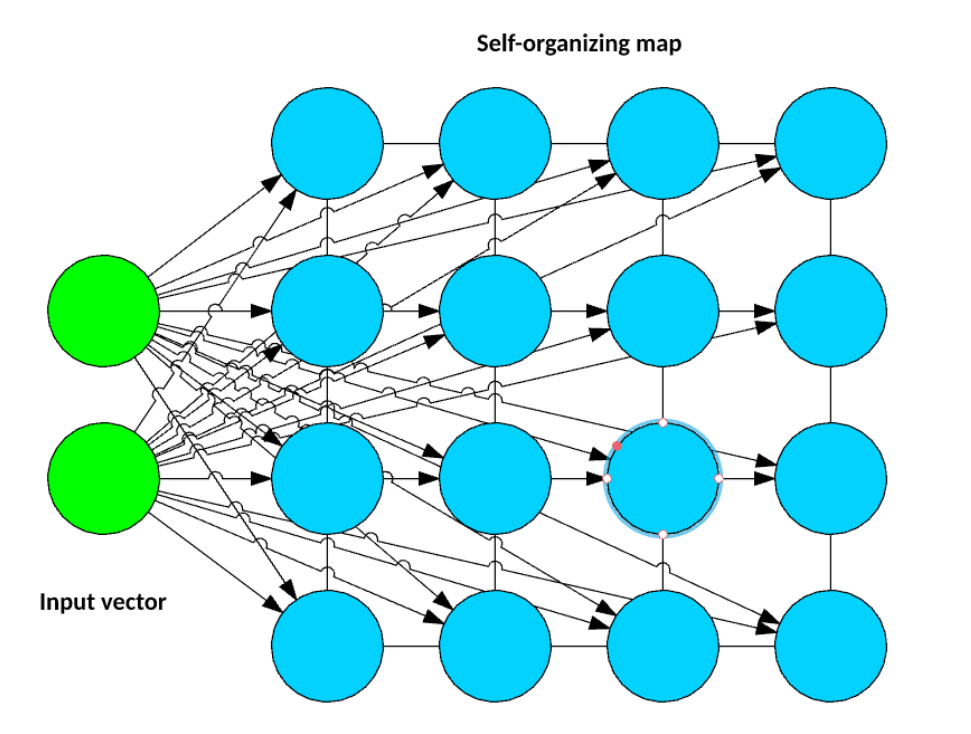
\includegraphics[width=0.5\textwidth]{Self_organizingMap.PNG}
        \caption{Self-organized map (SOM)}
        \label{fig:Self-organized map (SOM)}
    \end{figure}
    \textbf{Example applications:} Dimensionality reduction, clustering high-dimensional inputs to 2-dimensional output, radiant grade result, and cluster visualization
    \item \textbf{Autoencoders: } Autoencoders are a variant of artificial neural networks (ANNs) that consist of three layers: the input layer, the hidden layer, and the output layer. First, the input layer is encoded into the hidden layer using an appropriate encoding function. The number of nodes in the hidden layer is much less than the number of nodes in the input layer. This hidden layer contains a compressed representation of the original input. Finally, the output layer aims to reconstruct the input layer by using a decoder function.
    
    \begin{figure}[H]
        \centering
        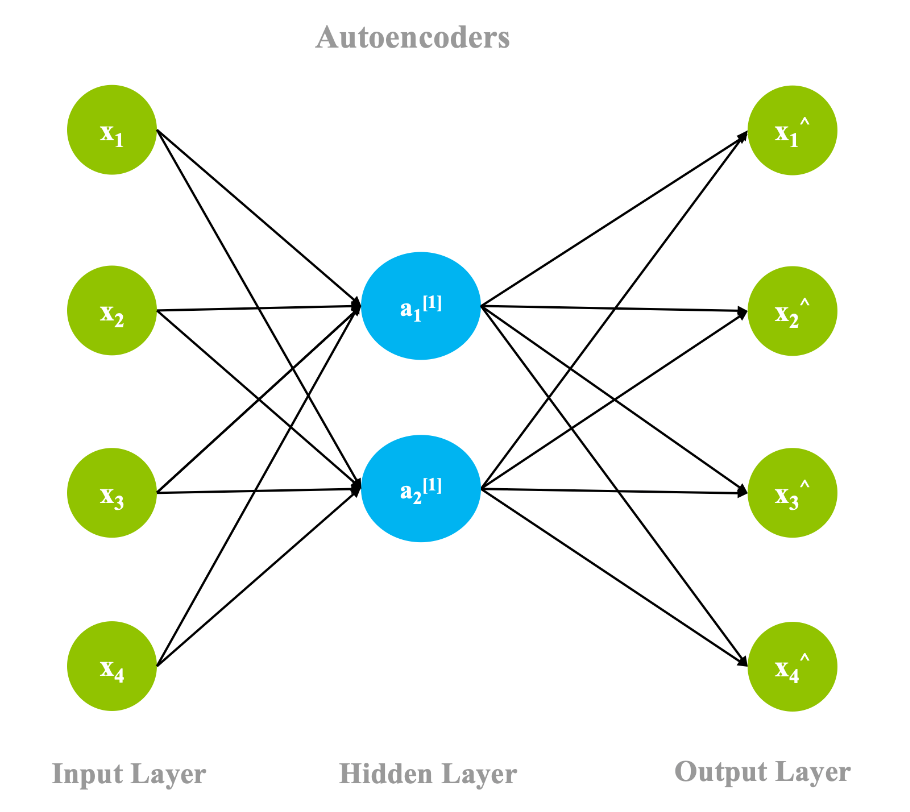
\includegraphics[width=0.7\linewidth]{tex/img/Autoencoders.PNG}
        \caption{Autoencoders \cite{madhavan2017deep}}
        \label{fig:Autoencoders}
    \end{figure}
   During the training phase, an error function is used to calculate the difference between the input and output layers, and the weights are adjusted accordingly to minimize the error. \\ 
    \textbf{Example applications:} Dimensionality reduction, data interpolation, and data compression/decompression.\\ 
    \item \textbf{Restricted Boltzmann Machines: } A Restricted Boltzmann Machine (RBM) is a type of neural network that consists of two layers: input and hidden layers. As depicted in figure \ref{fig:Restricted Boltzmann Machines}, every node in the hidden layer is connected to every node in the visible layer. Unlike traditional Boltzmann machines, where nodes in the input and hidden layers are interconnected, RBMs restrict the connections between nodes within a layer due to computational complexity.
    
    \begin{figure}[H]
        \centering
        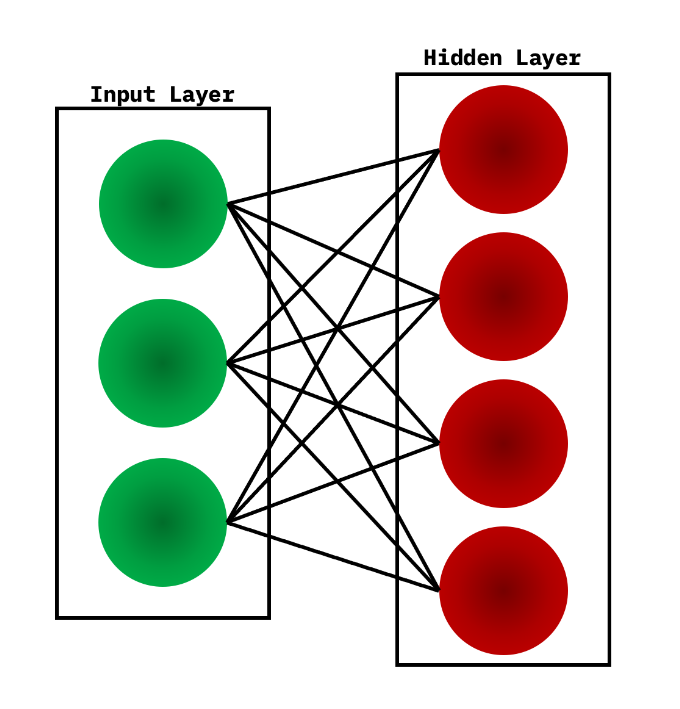
\includegraphics[width=0.6\textwidth]{RestrictedBoltzmannMachines.PNG}
        \caption{Restricted Boltzmann Machines \cite{madhavan2017deep}}
        \label{fig:Restricted Boltzmann Machines}
    \end{figure}
    During the training phase of RBMs, a stochastic approach is used to calculate the probability distribution of the training set. At the beginning of the training, each neuron is activated at random. The model also contains hidden and visible biases. The hidden bias is used in the forward pass to build the activation, while the visible bias helps in reconstructing the input. RBMs are also called generative models because the reconstructed input is always different from the original input. Additionally, due to the built-in randomness, the same predictions result in different outputs. RBMs is a deterministic model, and that makes it significantly different from Autoencoder. \cite{madhavan2017deep} \cite{alzubaidi2021review} \\
    \textbf{Example applications:} Dimensionality reduction and collaborative filtering.\\
    \item \textbf{Deep belief networks: } Deep belief networks (DBN) are multilayer networks that typically have several hidden layers, making them deep. Each pair of connected layers in a DBN is a Restricted Boltzmann Machine (RBM). The input layer of the DBN represents the raw sensory inputs, while each hidden layer learns abstract representations of this input. The output layer is treated differently and is responsible for network classification during training. The DBN is trained in two steps: unsupervised pretraining and supervised fine-tuning. \cite{sohn2021deep}, \cite{coates2011analysis}
    
    \begin{figure}[H]
        \centering
        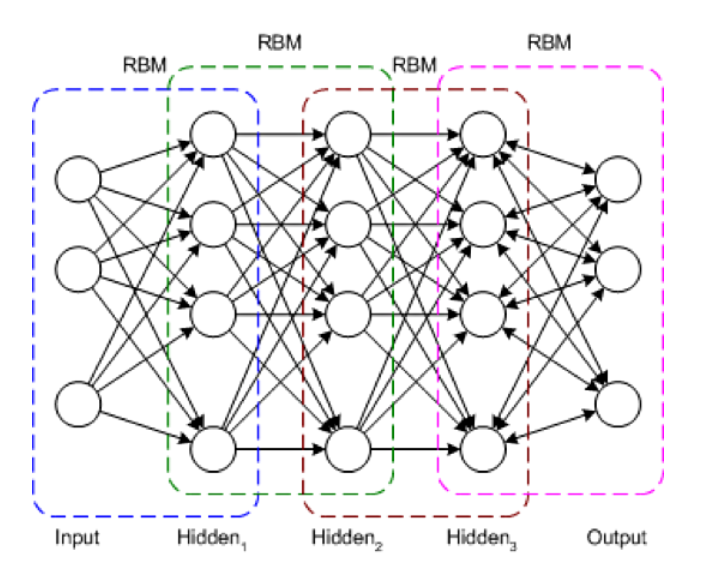
\includegraphics[width=0.7\textwidth]{DeepBelief_Networks.PNG}
        \caption{Deep belief networks architecture \cite{madhavan2017deep}}
        \label{fig:Deep belief networks}
    \end{figure}
    During unsupervised pretraining, each Restricted Boltzmann Machine (RBM) is trained to reconstruct its input. For instance, the first RBM reconstructs the input layer to the first hidden layer. Similarly, the next RBM is trained by using the outputs of the previous hidden layer as the inputs, and so on until each layer is pretrained. 

    After pretraining, fine-tuning commences, and the output nodes are assigned labels to give them meaning, i.e., to signify what they represent in the context of the network. The final step involves applying full network training using either gradient descent learning or back-propagation to complete the training process. \\
    \textbf{Applications: } object detection, information processing, natural language understanding processing, etc. \\
    \item \textbf{Deep stacking networks: } Deep stacking networks, also known as deep convex networks, are different from traditional deep learning frameworks. Although they consist of a deep network, they are actually a deep set of individual networks, each with its own hidden layers. 

    This architecture was developed to solve one of the main problems with deep learning: the complexity of training. Each layer in a deep learning architecture exponentially increases the complexity of training, but the DSN views training as a set of individual training problems, instead of a single problem.
    
    The DSN consists of a set of modules, each of which is a subnetwork in the overall hierarchy of the DSN. For example, in one instance of this architecture, three modules are created for the DSN. Each module consists of an input layer, a single hidden layer, and an output layer. Modules are stacked one on top of another, where the inputs of a module consist of the prior layer outputs and the original input vector. 
    
    This layering allows the overall network to learn more complex classifications than would be possible given a single module. \cite{deng2014tutorial}, \cite{madhavan2017deep}
    
    \begin{figure}[H]
        \centering
        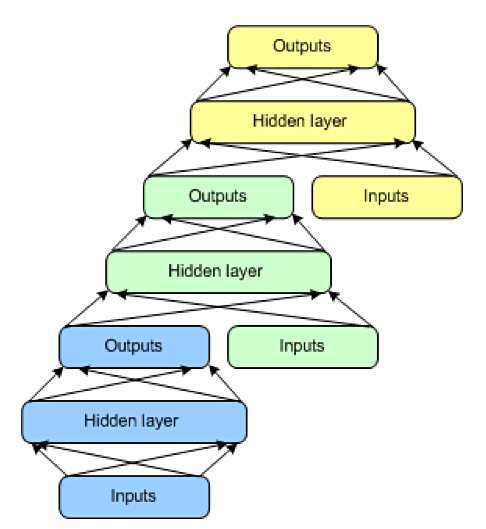
\includegraphics[width=0.5\textwidth]{DeepStackNetworks.PNG}
        \caption{Deep stacking networks architecture \cite{madhavan2017deep}}
        \label{fig:Deep stacking networks}
    \end{figure}
    \textbf{Example applications:} Information retrieval and continuous speech recognition
    

\end{itemize}
 % Wygodnie jest trzymać każdy rozdział w osobnym pliku.
\section{SOTA of object detection}
\subsection{Introduction to Object Detection}
\href{https://www.mathworks.com/discovery/object-detection.html#:~:text=Object%20detection%20is%20a%20computer,learning%20to%20produce%20meaningful%20results.}{Object detection} Object detection is a vital computer vision technique which is employed to identify instances of objects within images or videos. This technique is commonly implemented through the use of machine learning or deep learning algorithms, which are responsible for producing robust and accurate results. While humans are able to quickly recognize and locate objects of interest within visual data, the ultimate goal of object detection is to replicate this cognitive ability using computational methods. By detecting and localizing objects within visual data, object detection has become a crucial tool for various computer vision applications, including robotics, autonomous vehicles, and surveillance systems. \cite{zhao2019object}, \cite{ansari2020building}
\subsubsection{Why Object Detection}
Identifying and localizing objects within an image or video is called object detection and is a fundamental task in computer vision. It plays a pivotal role in various real-world applications, contributing to advancements in technology and enhancing our daily lives. The importance of object detection lies in its ability to enable machines to interpret and understand visual information, allowing them to make informed decisions and interact intelligently with the environment.\cite{pathak2018application}, 
\begin{enumerate}
    \item \textbf{Automation and Efficiency:} Object detection is a cornerstone in developing automated systems, empowering machines to perceive and respond to their surroundings. This is particularly crucial in industries such as manufacturing, where the automation of tasks, such as quality control and inventory management, leads to increased efficiency and reduced operational costs.
    \item \textbf{Enhanced Security and Surveillance:}  In the realm of security and surveillance, object detection is instrumental in identifying potential threats or anomalies. Surveillance cameras equipped with object detection algorithms can automatically detect and alert authorities to suspicious activities, enhancing public safety in crowded spaces, transportation hubs, and critical infrastructure.
    \item \textbf{Autonomous Vehicles:} The advent of autonomous vehicles relies heavily on object detection to interpret the dynamic environment. Cars equipped with object detection systems can identify pedestrians, vehicles, and obstacles, enabling safer navigation and reducing the likelihood of accidents.
    \item \textbf{Medical Imaging and Diagnosis:}  In the field of healthcare, object detection plays a vital role in medical imaging. It aids in detecting and localizing abnormalities in radiological images, facilitating early diagnosis and improving patient outcomes.
    \item \textbf{Retail and Customer Experience:} Object detection is utilized in retail for tasks such as inventory management, shelf monitoring, and cashierless checkout systems. These applications streamline operations and enhance customer experience by reducing waiting times and optimizing stock levels.
\end{enumerate}

\textbf{Real-world Scenarios:}\\
\begin{enumerate}
    \item \textbf{Smart Cities:} Object detection is integral to developing smart cities. It can be used in urban environments for traffic management, waste management, and monitoring public spaces, contributing to more efficient and sustainable urban living.
    \item \textbf{Search and Rescue Operations:} In disaster-stricken areas, object detection aids in search and rescue operations by identifying and locating individuals needing assistance. Drones equipped with object detection capabilities can quickly cover large areas, improving rescue efforts' efficiency.
    \item \textbf{Environmental Monitoring: } Object detection is applied in environmental science for monitoring wildlife, tracking deforestation, and studying biodiversity. It enables researchers to gather crucial data for conservation and ecological studies.
    \item \textbf{Augmented Reality:} Object detection is a key component in augmented reality applications, where virtual elements are seamlessly integrated with the real world. This technology enhances user experiences in gaming, education, and various interactive scenarios.
\end{enumerate} \cite{ansari2020building}, \cite{pathak2018application}

\subsection{Object detection stage}
Object detection can be classified into two stages according to the detection process steps:
\begin{itemize}
    \item \textbf{One-stage detector}  is a simple regression problem that takes input and learns probability classes and bounding box coordinates. YOLO, YOLO v2, SSD, RetinaNet, etc., fall under one-phase detectors. Object detection is an advanced form of imaging classification where a neural network predicts objects in an image and draws attention to them in the form of bounding boxes. \cite{oneStage}
    \item \textbf{Two-stage detector} A two-stage detector completes detection in two steps. In the first step, regional design networks are used to create areas of interest with a high probability of being objects. In the second step, object detection is performed, which includes the final classification and regression of the bounding box of the detected objects. RCNN, Fast RCNN, SPPNET, Faster RCNN, etc., are some of the two-stage detectors. \cite{du2020overview}
\end{itemize}

\begin{figure}[H]
    \centering
    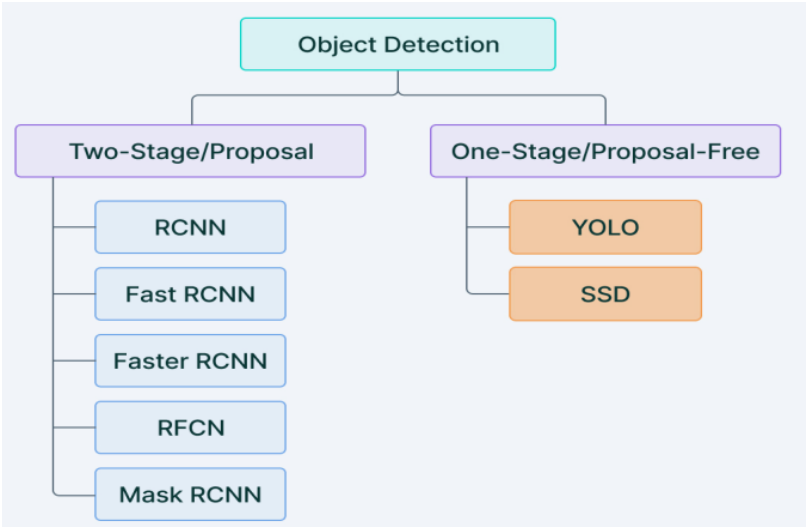
\includegraphics[width=0.7\textwidth]{ObjectDetection_Stage.PNG}
    \caption{Stage  or classification of Object Detection}
    \label{fig: Stage of Object Detection}
\end{figure}

\subsection{Two-Stage/Proposal: }
  Two-stage object detection algorithms typically have two steps: region proposal and object classification or refinement. One popular framework is the region-based Convolutional Neural Network (R-CNN) and its variants.\cite{du2020overview}, \cite{ansari2020building}
\subsubsection{Region-Based Convolutional Neural Network: } \underline{\textcolor{blue}{\href{https://arxiv.org/pdf/1311.2524.pdf}{R-CNN}}}
A Region-Based Convolutional Neural Network (R-CNN) is a type of neural network specifically designed to detect objects in images. R-CNN uses region proposals generated by a selective search (SS) approach to pre-compute the priors. Since the features between these regions are not shared, we need to extract features individually for each region of interest (RoI) generated using an SS approach. Unlike other neural networks, R-CNNs are designed not only to classify objects but also to locate and delineate their boundaries within the image.
The R-CNN architecture was first proposed in 2014 by Ross Girshick, Jeff Donahue, Trevor Darrell, and Jitendra Malik in their paper titled "Rich Feature Hierarchies for Accurate Object Detection and Semantic Segmentation." Since then, the architecture has undergone several iterations, including Fast R-CNN, Faster R-CNN, and Mask R-CNN.
        
    \begin{figure}[H]
         \centering
         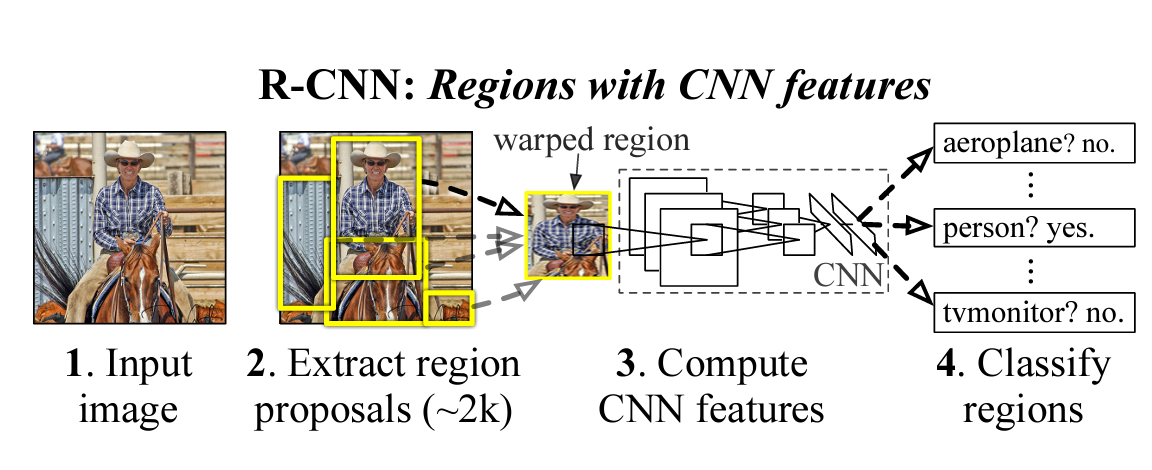
\includegraphics[width=0.6\textwidth]{R_CNN.PNG}
         \caption{R-CNN Model(Source:\cite{girshick2014rich})}
            \label{fig: R-CNN Model}
    \end{figure}
\textbf{R-CNN comprises of the following three modules:}\\
        \begin{enumerate}
            \item \textbf{Region proposal: } The R-CNN algorithm starts by identifying regions in an image that may contain objects. These regions are known as region proposals. They are referred to as proposals because they may or may not contain objects, and the goal of the learning function is to remove areas that do not contain objects. Region proposals are bounding boxes around the objects.
            \item \textbf{Feature extraction:} To identify objects in an image, the first step is to crop out the region proposals and resize them. These resized images are then sent through a standard CNN for feature extraction. The original research paper employed AlexNet for this purpose. The CNN extracts 4,096-dimensional feature vectors from each region.
            \item  \textbf{Classifier: } The extracted features are classified by using the standard classification algorithms, such as the linear SVM model 
        \end{enumerate}
R-CNN was the first successful deep learning–based object detection system, but it suffered a serious issue concerning performance. Its time performance problem is because of the following:
    \begin{itemize}
         \item For feature extraction, each region proposal undergoes approximately 2,000 passes per image in the CNN.
        \item Three models are trained: CNN for feature extraction, classifier for image class prediction, and regression for bounding box refinement. Training is compute-intensive, increasing computation time.
        \item Due to the large number of regions, CNN predictions are slow for each proposal.
    \end{itemize}
        
\subsubsection{Fast R-CNN:} In 2015, Ross Girshick from Microsoft proposed a single model called "Fast R-CNN" to overcome the limitations of R-CNNs. This model learns and outputs region proposals and classifications directly, resulting in higher mAP on PASCAL compared to R-CNN.  \href{https://arxiv.org/pdf/1504.08083.pdf}{\textcolor{blue}{Fast R-CNN:}}
\href{https://medium.com/alegion/deep-learning-for-object-detection-and-localization-using-fast-r-cnn-85d52e3928a1}{\textcolor{blue}{[2]}}\\
Fast R-CNN trains a deep VGG-16 network that is significantly faster than R-CNN (9x faster during training and 213x faster at test time). The model achieves this speed by evaluating the network and extracting features for the entire image once, instead of extracting features from each region of interest (RoI) as in R-CNN. To extract features from RoIs, Fast R-CNN uses the concept of RoI pooling, which is a special case of pyramid pooling used in SPPNet. 

RoI pooling provides a feature vector of the desired length that is then used for classification and localization. This method is more efficient than R-CNN because the computations for overlapping regions are shared. Overall, Fast R-CNN significantly improves the speed and performance of object detection models.
        

\textbf{Building blocks of Fast R-CNN:}
    \begin{enumerate}
        \item Region proposal network
        \item Feature extraction using CNN
        \item RoI pooling layer: This is where the real magic of Fast R-CNN happens
        \item Classification and Localization
    \end{enumerate}
        
    \begin{figure}[H]
        \centering
        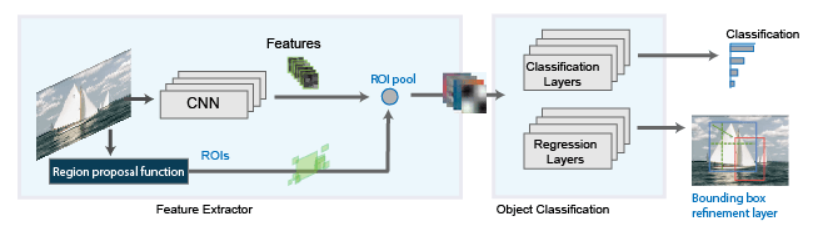
\includegraphics[width=1\textwidth]{Fast_RCNN_ARch.PNG}
        \caption{Architectural Design of Fast R-CNN \cite{girshick2014rich}}
        \label{fig: Fast R-CNN}
    \end{figure}
\href{https://www.mathworks.com/help/vision/ug/getting-started-with-r-cnn-fast-r-cnn-and-faster-r-cnn.html#d117e11449}{\textcolor{blue}{Image Source}}
        
The region proposal network and feature extraction modules work similarly to the ones used in R-CNN. However, instead of passing each cropped and re-scaled RoI (region of interest), the entire input image is processed through a feature extractor like VGG-16. This produces a convolutional feature map. The features (i.e., the convolutional feature map) are then combined with the region proposal network, which uses a selective search approach to create a fixed-length feature vector in the RoI pooling layer. These feature vectors are then passed along to the classification and localization modules. The classification module classifies K+1 (1 for background) object classes using a softmax probability. The localization module outputs four real-valued numbers for each K object class. \cite{girshick2015fast}
\subsubsection{Faster R-CNN}
Faster R-CNN is an improved version of Fast R-CNN from the training speed and detection accuracy perspectives.
Faster R-CNN added what they called a Region Proposal Network (RPN) in an attempt to get rid of the selective search algorithm and make the model completely trainable end-to-end.

\begin{figure}[H]
    \centering
    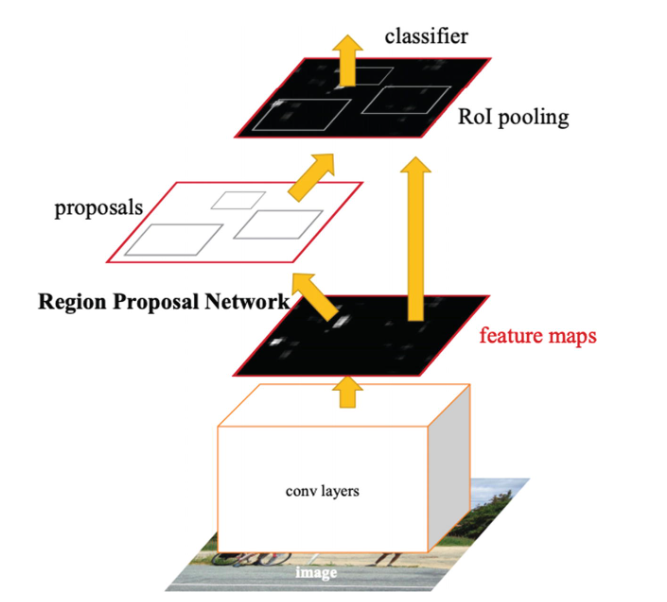
\includegraphics[width=0.7\textwidth]{Faster_RNN.PNG}
    \caption{Architectural Design of Faster R-CNN \cite{ansari2020building}}
    \label{fig:Faster R-CNN}
\end{figure}

\begin{enumerate}
    \item \textbf{Region Proposal Network: } An RPN is a fully convolutional neural network that predicts object bounds and objectness scores simultaneously at each position of the image.
    An RPN is a deep CNN that takes an image input and generates the output as a set of rectangular object proposals. Each rectangular proposal has an “objectness” score.
    
    \begin{figure}[H]
        \centering
        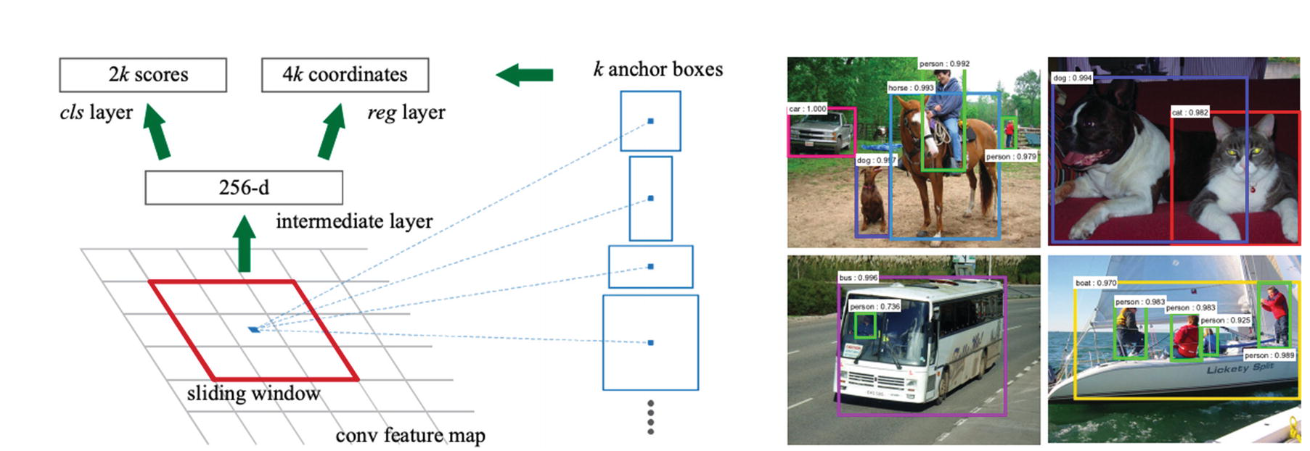
\includegraphics[width=1\textwidth]{RPN.PNG}
        \caption{Region Proposal Networks (RPN) [image source: \cite{chen2018enhanced}}
        \label{fig:RPN}
    \end{figure}
    RPN has a classifier and a regressor. The concept of anchors has been introduced, which refers to the central point of the sliding window.
    The classifier determines the probability of a proposal having the target object. Regression
    regresses the coordinates of the proposals.
    At each sliding window location, the algorithm predicts multiple region proposals. If the maximum number of proposals at each window location is k, then the total number of bounding box coordinates will be 4k, while the number of object classes will be 2k. One of the classes will indicate the probability of an object being present in the region, and the other will indicate the probability of no object being present. These region boxes at each window are referred to as anchors.\\
    \item \textbf{Fast R-CNN: } The Faster R-CNN consists of two parts, with the second part being the detection network. This part is identical to the Fast R-CNN, which was described earlier. The Fast R-CNN uses input from the RPN to detect objects in images.
\end{enumerate} \cite{ansari2020building}, \cite{salvador2016faster}


\subsubsection{Mask R-CNN}
\textcolor{red}{\href{https://arxiv.org/pdf/1703.06870.pdf}{\textcolor{blue}{Mask R-CNN}}}
The Mask R-CNN extends the Faster R-CNN. The Mask R-CNN adds another branch for the object class, bounding box coordinates, and predicting an object mask.
Here is how the Mask R-CNN differs from its predecessor, the Faster R-CNN:
\begin{itemize}
    \item The Faster R-CNN algorithm produces two main results, namely: a predicted class label and the coordinates of the bounding box for the object of interest in an image.
    \item The Mask R-CNN has three outputs: a class label, bounding box coordinates, and an object mask.
\end{itemize}
The Mask R-CNN algorithm classifies each pixel of an image into a specific category, without distinguishing between individual object instances. To achieve this, it employs a technique known as pixel-to-pixel alignment between the output and input layers of the neural network. The classification of each pixel is then used to determine the masks in the region of interest (ROI).

\begin{figure}[H]
    \centering
    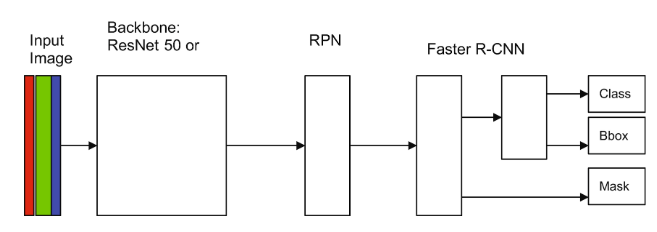
\includegraphics[width=1\textwidth]{MaskR-CNN.PNG}
    \caption{Mask R-CNN network architecture \cite{he2017mask}}
    \label{fig:MaskR-CNN}
\end{figure}
As shown in Figure \ref{fig:MaskR-CNN}, the network consists of three components \textbf{modules—backbone, RPN, and output head}.
\begin{itemize}
    \item \textbf{Backbone} The backbone networks are commonly seen in object detection model architectures. The original paper describes using ResNet-50 and ResNet-101[ \textcolor{red}{\href{https://arxiv.org/pdf/1612.03144.pdf}{Ref1}} ]
    The backbone’s main role is feature extraction.
    In addition to ResNet, a feature pyramid network (FPN) is also utilized to extract the feature details of the image.
    \begin{figure}[H]
        \centering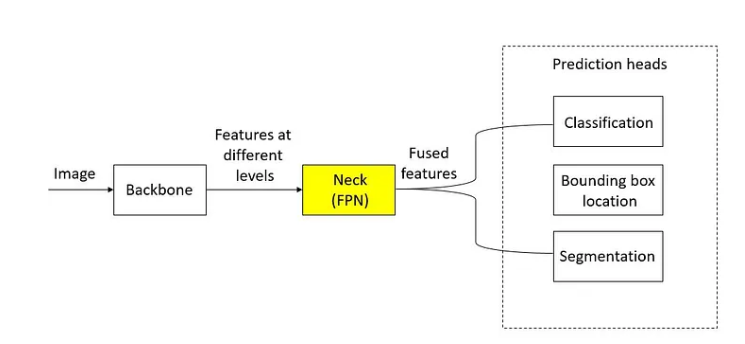
\includegraphics[width=1\textwidth]{BackBone_FPN.PNG}
        \caption{BackBone and FPN Tuning architecture \protect\href{https://medium.com/@freshtechyy/fusing-backbone-features-using-feature-pyramid-network-fpn-c652aa6a264b}{[\textcolor{black}{Ref}} ]}\cite{zhu2022improved} 
    \end{figure}
The FPN consists of decreasing-size layers of a CNN, in which case each forward layer has fewer neurons.

        \item \textbf{Feature Pyramid Network (FPN): } is a neck network that combines features of different resolutions obtained from a backbone network, such as ResNet. A CNN-based backbone applies convolution layers to an input image, which results in a set of feature maps with decreasing resolution due to pooling or convolution with a stride different from one.\\
        The FPN consists of a bottom-up and top-down pathway. In the bottom-up pathway, a backbone network, such as ResNet, extracts features with diminishing spatial resolution.
        As the levels of resolution decrease, the semantic meaning of the feature maps increases, as indicated by the blue thickness of the box boundaries.\\
        The feature maps are fused in the top-down pathway to incorporate rich semantic meaning and precise spatial information, as illustrated in the figure. \ref{fig:FPN_Arch} below. \cite{lin2017feature}
        \begin{figure}[H]
            \centering
            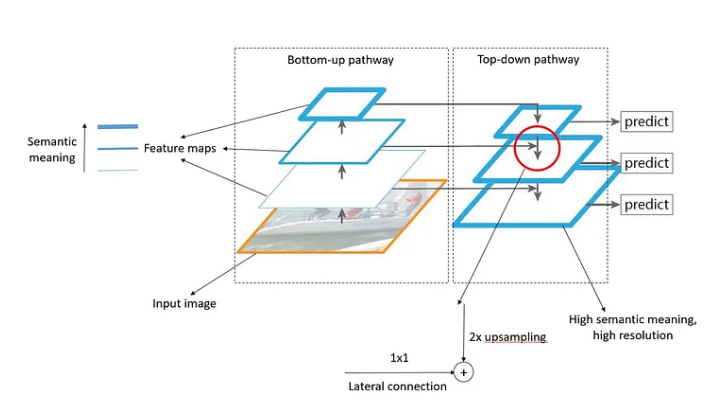
\includegraphics[width=0.7\textwidth]{FPN_Top_bott.PNG}
            \caption{Feature Pyramid Network (FPN) \cite{lin2017feature}}
            \label{fig:FPN_Arch}
        \end{figure}
         \item \textbf{Output Head: } The last module consists of the Faster R-CNN with an additional output branch. \cite{he2017mask}
\end{itemize}
   
\subsection{One stage detector: } 
They can process images in real-time and are suitable for applications where low latency is crucial, such as real-time object detection in video streams or robotics.

\subsubsection{Single-Shot Multibox Detection: }

SSD is primarily designed to solve object detection problems in real-time. An R-CNN and its variants are detectors that work in two stages. They have two specialized networks: one creates the region proposals to predict bounding boxes, and the other predicts the object classes. These detectors are relatively accurate but have a high computational cost. As a result, an R-CNN is not ideal for detecting objects in real-time streaming videos.
A single-shot object detector predicts object classes and bounding boxes in one pass or single forward-pass\cite{liu2016ssd} 
\begin{itemize}
    \item \textbf{SSD Network Architecture: } The SSD approach is a method that uses a feed-forward convolutional network to generate a set of fixed-size bounding boxes and scores, which helps detect the presence of object class instances in those boxes. A non-maximum suppression step is performed in the final stage to obtain the ultimate detections. \\
    \begin{itemize}
        \item \textbfThe {Single Shot MultiBox Detector (SSD)} is a novel object detection framework that adopts grid-based image division instead of the conventional sliding window approach. The SSD approach divides the image into a grid pattern, where each grid cell is responsible for detecting objects within its corresponding region of the image. The objective of object detection is to predict the class and location of an object within its region. In case no object is present, the region is considered a background class, and the location is consequently ignored.

        During the training process, SSD requires only an input image and ground truth boxes for each object. In a convolutional manner, a small set of default boxes of different aspect ratios is evaluated at each location in several feature maps with different scales. For instance, 8x8 and 4x4 in (b) and (c). For each default box, SSD predicts the shape offsets and confidences for all object categories (c1, c2, ..., cp). Notably, these default boxes are first matched to the ground truth boxes during training.
        \begin{figure}[H]
            \centering
            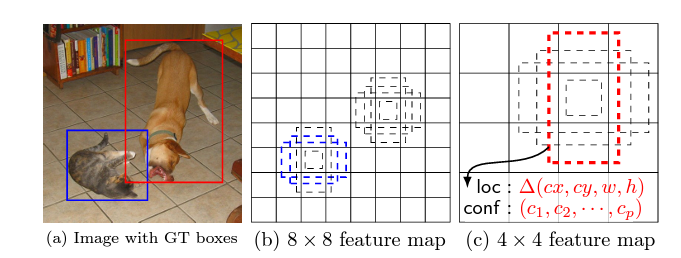
\includegraphics[width=\textwidth]{SSD_GridCell.PNG}
            \caption{SSD:Single Shot Multi-Box Detector \textcolor{red}{\protect\href{https://arxiv.org/pdf/1512.02325.pdf}{image source: \cite{liu2016ssd}}}}
            \label{fig:SSD_grid}
        \end{figure}
        
        \item \textbf{Anchor Boxes:} Object detection is a process by which we aim to identify and locate objects as they appear within an image. This process is different from image classification because there may be multiple objects of the same or different classes present in the image, and object detection seeks to predict all of these objects accurately. In object detection, we use anchor boxes to help locate these objects in the image.
        Object detection models tackle this task by breaking the prediction step into two pieces: 
        \textcolor{red}{\href{https://blog.roboflow.com/what-is-an-anchor-box/}{Ref: Anchor-box}}
        \begin{enumerate}
            \item First, they predict a bounding box through regression and
            \item Second, by predicting a class label through classification.
        \end{enumerate}
        
        \begin{figure}[H]
            \centering
            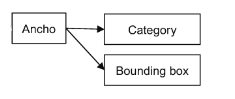
\includegraphics[width=0.2\textwidth]{Anchor.PNG}
            \caption{Anchor}
            \label{fig:anchor}
        \end{figure}
       To detect and locate multiple objects in an image, modern object detection models such as SSD, EfficientDet, and the YOLO models use anchor boxes as a starting point and then make adjustments accordingly. These anchor boxes are predetermined, and each one is responsible for a specific size and shape within a grid cell.

      Anchors are rectangular shapes that are set at each convolution point of the feature map. In SSD, each grid cell can have multiple anchors or prior boxes assigned to it.
            
        
        In Figure \ref{fig: anchor box}, there are five rectangular anchors (shown in red outlines) set at a point (shown in blue).
        \begin{figure}[H]
            \centering
            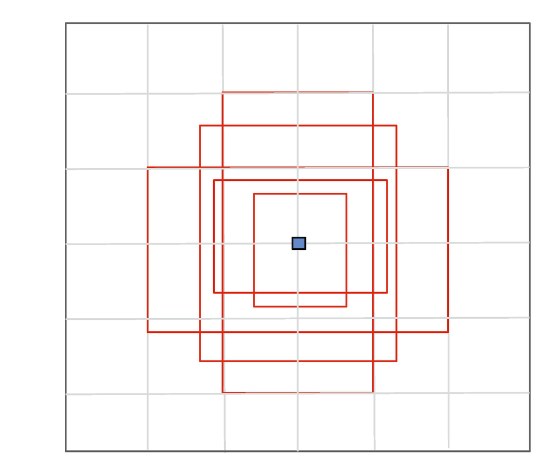
\includegraphics[width=0.5\textwidth]{Anchor_Boxes.PNG}
            \caption{Anchor Boxes}
            \label{fig: anchor box}
        \end{figure}
        In Single Shot Detector (SSD) network, multiple anchor boxes are selected at each location. These anchors serve as detectors, and the different sizes of these detectors enable the detection of objects of varying sizes. Smaller detectors can detect small objects, while larger detectors are capable of detecting larger objects.\\
        \item SSD does not use k-means to determine the anchor boxes, unlike some other object detection algorithms. Instead, it employs a mathematical formula to compute the anchor sizes. As a result, the sizes of SSD's anchor boxes are not dependent on the dataset used. In the SSD paper, these anchor boxes are referred to as "default boxes".\textcolor{red 
        {\href{https://arxiv.org/pdf/1512.02325.pdf}{Ref:Original Paper}}.  \href{https://machinethink.net/blog/object-detection/}{SSD}
        
        It is worth mentioning that in SSD (Single Shot Multibox Detector), anchors are predetermined and set as constants. At each convolution point, a set of fixed "default anchors" is placed. These anchors are associated with a set of default bounding boxes for multiple feature maps at the top of the network. They are laid out in a convolutional manner, tiling the feature map so that the position of each box relative to its corresponding cell remains fixed.
            \end{itemize}
    \item \textbf{Model Architecture: } An SSD neural network consists of two components: \textbf{base network and prediction network.}
    \begin{enumerate}
        \item \textbf{Base network:} The base network is a type of deep convolutional network that is used for feature extraction from input images. It is typically created by removing the fully connected layer of existing networks such as ResNet or VGG. In the case of SSD, the base network is truncated before any classification layer.
        \item \textbf{Detection network:} To the base network, attach some extra convolutional layers that will actually do the prediction of bounding boxes and object classes. 
        \begin{figure}[H]
        \centering
        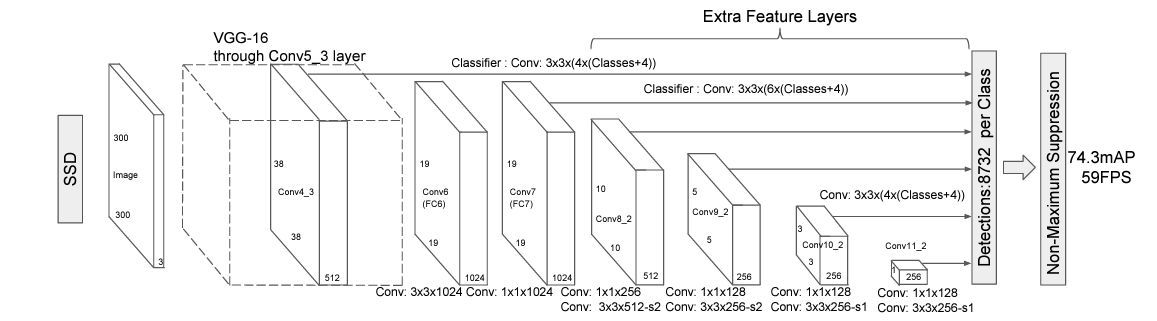
\includegraphics[width=\textwidth]{SSD_ARch.PNG}
        \caption{single shot detection models: SSD \cite{liu2016ssd}}
        \label{fig: single shot detection models: SSD}
        \end{figure}
    The detection network is characterized by the following features: \cite{liu2016ssd}
        \begin{itemize}
            \item TThe layers in the network gradually decrease in size, enabling the detection of objects at multiple scales.
            \item  Each feature layer in the network uses a different convolutional model for predicting detections.
            \item By adding a new feature layer (or using an existing layer from the base network), a fixed set of detection predictions can be generated using a set of convolutional filters
        \end{itemize}
    \end{enumerate}
    \item \textbf{Matching System: } When training, we must choose default boxes that correspond to ground truth detection and train the network accordingly. For each ground truth box, we choose from default boxes that vary in location, aspect ratio, and scale.  The SSD uses IoU (intersection over union) to match the default boxes with the ground truth. This is done by determining the overlap between them. The IoU-based overlap is also known as the Jaccard overlap. If the overlap between the default box and the ground truth is 0.5 or more, it is considered a match. This process of matching is repeated at each layer, which allows the network to learn at scale. Initially, the SSD uses the default boxes as predictions and then tries to regress and come closer to the ground truth bounding boxes. \cite{ansari2020building}, \cite{liu2016ssd}

\end{itemize}

\subsection{Object Detection Evaluation Metrics}
Object detection is a computer vision task where the goal is to identify and locate objects of interest within an image or a video. Several evaluation metrics are commonly used to assess the performance of object detection algorithms. The following are some of the detection metrics:
\subsubsection{Intersection over Union (IoU)}
Intersection over union (IoU), also known as the Jaccard index, is one of the most commonly used evaluation metrics in object detection algorithms. It is used to evaluate the performance of object detection by comparing the ground truth bounding box to the predicted bounding box and IoU.
When it comes to object detection, we create training sets by drawing bounding boxes around objects to label them. These bounding boxes are also known as ground truth in the training set. During the model learning process, the object detection algorithm predicts bounding boxes and then compares them with the ground truth. To determine the accuracy of the predicted bounding box, we use intersection over union (IoU) to evaluate to what extent the predicted bounding box overlaps with the ground truth.\cite{ansari2020building}, \cite{bfortuner_mlglossary}, \cite{liu2016ssd}

\begin{figure}[H]
    \centering
    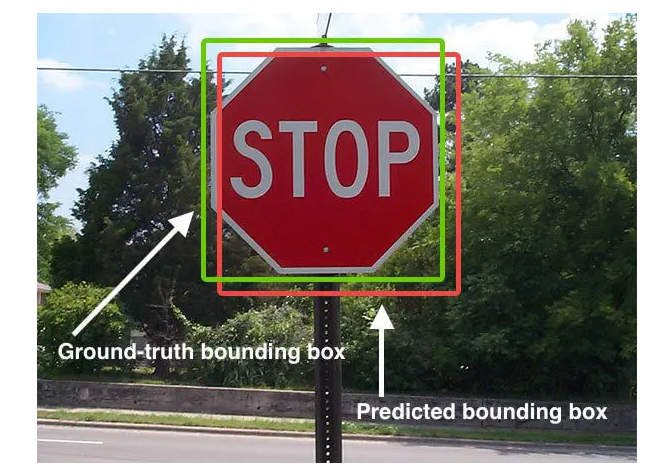
\includegraphics[width=0.6\textwidth]{Intersection_overUnion_(IoU).PNG}
    \caption{The predicted bounding box and Ground-truth bounding box \cite{ansari2020building}}
    \label{fig:PBGTB}
\end{figure}

\textbf{Computing Intersection over Union can therefore be determined as:}\\

\begin{figure}[H]
    \centering
    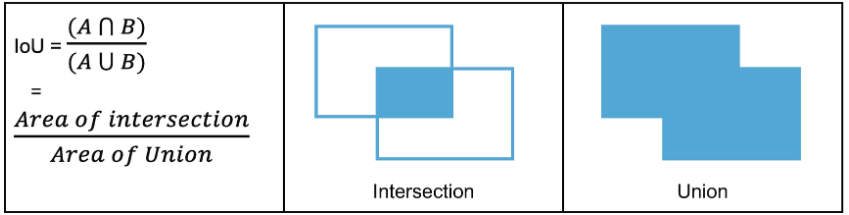
\includegraphics[width=0.6\textwidth]{Intersection_OverUnion.PNG}
    \caption{Intersection OverUnion}
    \label{fig:Intersection_OverUnion}
\end{figure}

\subsubsection{Mean Average Precision (mAP)}
Mean Average Precision (mAP) is a frequently employed metric for evaluating the effectiveness of object identification and segmentation systems. Several object recognition techniques, including Faster R-CNN, MobileNet SSD, and YOLO, utilize mean Average Precision (mAP) as a metric to assess the performance of their models. The mean Average Precision (mAP) is utilized in various benchmark challenges, including Pascal, VOC, COCO, and others. The mean of Average Precision (AP) values are computed by averaging the AP values obtained for recall levels ranging from 0 to 1.\cite{padilla2020survey}, \cite{ansari2020building},  \\
mAP formula is based on the following sub metrics:
\begin{itemize}
    \item Confusion Matrix
    \item Intersection over Union(IoU)
    \item Recall,
    \item Precision
\end{itemize}
\begin{enumerate}
    \item \textbf{Confusion Matrix: }A confusion matrix is a table that is often used to evaluate the performance of a classification algorithm on a set of labeled data for which the true values are known. It provides a summary of the classification results, breaking down the predicted and actual classes into four categories: true positives (TP), true negatives (TN), false positives (FP), and false negatives (FN). \cite{padilla2020survey}, \cite{li2019analysis}
    \begin{itemize}
        \item \textbf{True Positives (TP): } This is when the model accurately predicts a label that matches the ground truth.\\
        \item \textbf{True Negatives (TN): } This is when the model does not predict the label and is not part of the ground truth.\\
        \item  \textbf{False Positives (FP): } This is when the model predicts a label, but it is not a part of the ground truth (Type I Error).\\
        \item \textbf{False Negatives (FN): } Finally, this is when the model does not predict a label, but it is part of the ground truth. (Type II Error).
        \begin{figure}[H]
            \centering
            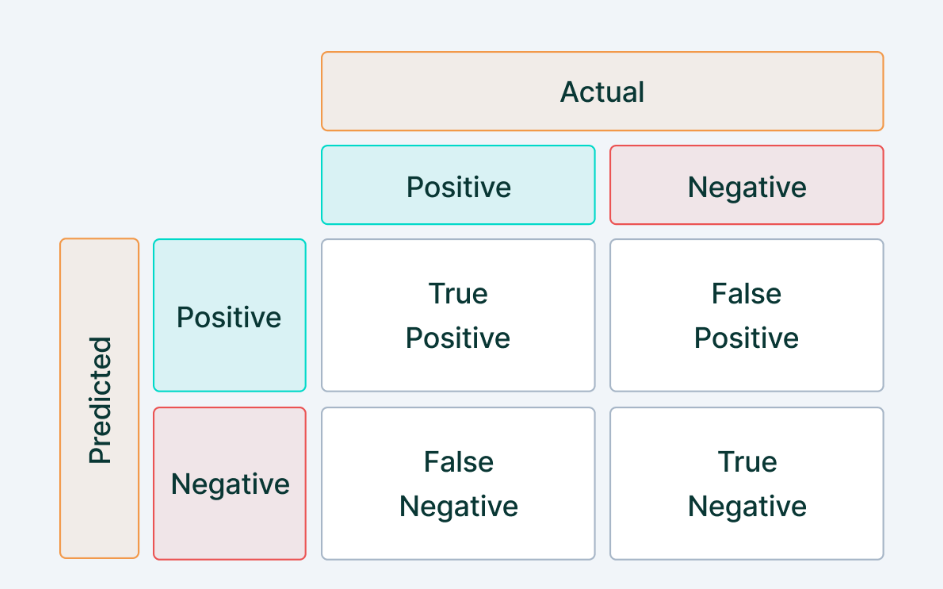
\includegraphics[width=0.7\textwidth]{confusion_matrix.PNG}
            \caption{Confusion matrix table}
            \label{fig:Confusion_Matrix}
        \end{figure}
    \end{itemize}
    \item \textbf{Precision: } Precision measures how well you can find true positives(TP) out of all positive predictions. (TP+FP).
    $$Precision=\frac{TP}{TPTP+FP}$$

    \item \textbf{Recall: } Recall measures how well you can find true positives(TP) out of all predictions(TP+FN).
    $$Recall=\frac{TP}{TPTP+FN}$$
    
  
\end{enumerate}


\subsection{YOLO}
YOLO is one of a real-time object detection algorithm that is aimed and designed to be fast and accurate. It uses a single convolutional neural network to simultaneously predict the bounding boxes along with class probabilities of objects in an image. What sets YOLO apart from other object detection algorithms is that it trains on the full image and is set up to solve regression problems. This means that it does not require a complex processing pipeline, which makes it extremely fast.YOLO is a system that simplifies object detection by treating it as a single regression problem. It predicts bounding box coordinates and class probabilities directly from image pixels. With YOLO, you can detect objects in an image with just one look and get information about what objects are present and where they are located. \cite{redmon2016you}, \cite{ansari2020building}

\subsubsection{Detection Algorithm}
The YOLO design enables end-to-end training and real-time speeds while maintaining high average precision. \\
It divides the image into an SxS grid and for each
grid cell predicts \textbf{B} bounding boxes, confidence for those boxes,
and C-class probabilities. These predictions are encoded as a tensor.
\[
S x S x (B*5 + C)
\]
\\
\begin{figure}[H]
    \centering
    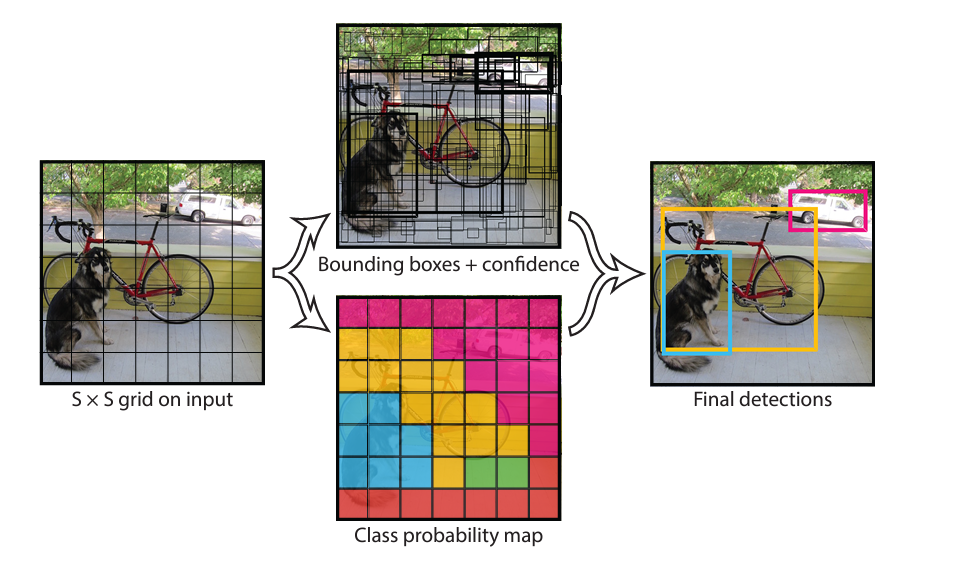
\includegraphics[width=0.8\textwidth]{YOLO_Detection.PNG}
    \caption{YOLO Model \cite{redmon2016you}}
    \label{fig:YoloV1_Model}
\end{figure}

Each bounding box consists of 5 predictions: x, y, w, h,
and confidence. confidence scores reflect how confident the model is.
\[
Confidence =Pr(Object)*IOU_{pred}^{truth}
\]
\subsubsection{YOLO Architectural Design}
The YOLO network architecture is inspired by GoogLeNet and is composed of 24 convolutional layers and 2 fully connected layers for image classification. The YOLO network uses 1x1 reduction layers followed by 3x3 convolutional layers, in contrast to the inception modules used in GoogLeNet. The full network is shown in Figure[\ref{fig:YOLO_arc}].
\begin{figure}[H]
    \centering
    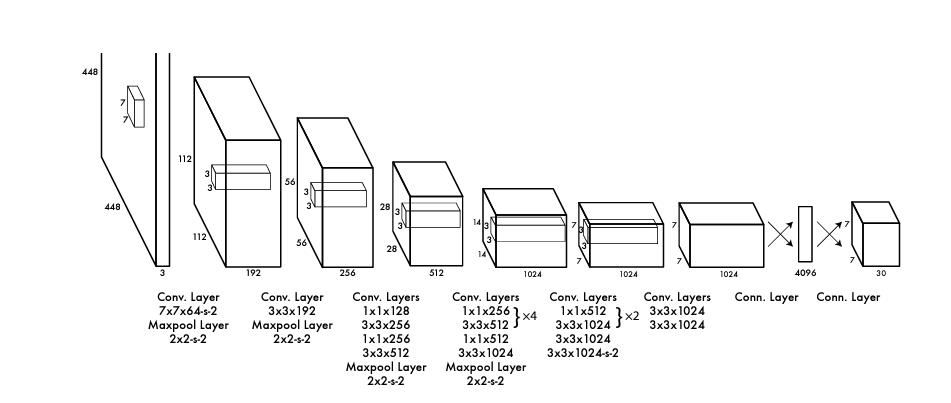
\includegraphics[width=\textwidth]{Yolo_Arch.PNG}
    \caption{YOLO Model (Image source Original paper \cite{redmon2016you})}
    \label{fig:YOLO_arc}
\end{figure}
The convolutional layers were pre-trained on the ImageNet 1000-class competition dataset. Following an average-pooling layer and a fully connected layer, YOLO uses the first 20 convolutional layers from Figure \ref{fig:YOLO_arc} for pretraining. The final layer predicts both class probabilities and bounding box coordinates. A leaky rectified linear activation is used for all layers except the final layer, which uses a linear activation function.
 \[
 \phi(x)=\begin{cases}
           x, & \text{if } x>0 \\
          0.1x, & \text{otherwise}
      \end{cases}
\]

\subsubsection{Limitations of YOLO}
\begin{itemize}
    \item It struggles with small objects that come in groups, such as flocks of birds.
    \item It can predict only one class of objects within a cell grid.
    \item It does not predict well if the object has an unusual aspect ratio that was not seen in the training set.
    \item The accuracy of YOLO is lower than that of Faster R-CNN and some of the state-of-the-art algorithms.
\end{itemize}

\subsection{Transfer Learning and Pre-trained Models:}

Transfer learning is a technique in deep learning where a pre-trained model for a particular task is used as a starting point for another model that performs a similar task. This approach provides a faster and easier way to update and retrain a network as compared to training a network from scratch. It is commonly used in various applications, such as object detection, image recognition, and speech recognition. \cite{you2021logme}

Transfer learning is a popular technique because:
\begin{itemize}
    \item Using transfer learning, you can train models with less labeled data by utilizing popular models that have already been trained on large datasets.
    \item  It can reduce training time and computing resources. With transfer learning, the weights are not learned from scratch because the pre-trained model has already learned the weights based on previous learning.
    \item You can take advantage of model architectures developed by the deep learning research community, including popular architectures such as GoogLeNet and ResNet.
\end{itemize}
\begin{figure}[H]
     \centering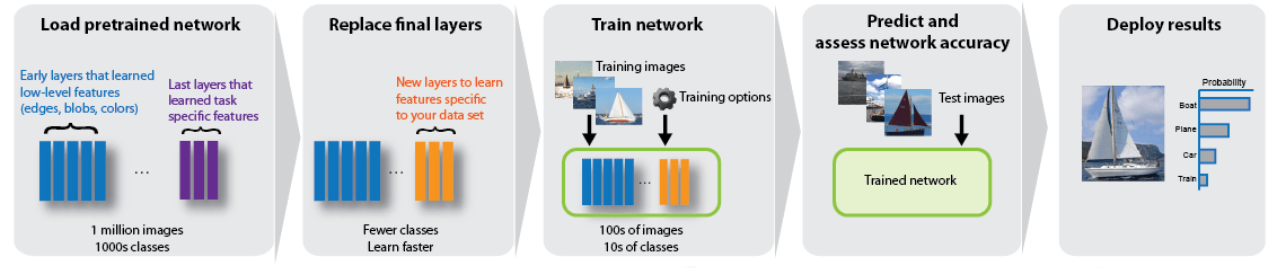
\includegraphics[width=1\linewidth]{Transfer_Learning_Model.PNG}
    \caption{Transfer Learning (Image source: \cite{murugan2021diconet})}
    \label{fig: Transfer Learning}
\end{figure}
\subsubsection{Pre-trained Model}
There are several pre-trained models available for object detection. Below are some of the most popular ones:\\
\begin{itemize}
    \item Alexnet, googlenet(ImageNet), goolgenet(Places365), resnet18, resnet50, resnet101, vgg16, vgg19, inceptionv3, inceptionresnetv2, squeezenet, densenet201, mobilenetv2, shufflenet, xception, nasnetmobile, nasnetlarge. 
\end{itemize}

When selecting a neural network, it's crucial to take into account its accuracy, speed, and size. Usually, there's a trade-off between these factors. To make a well-informed decision, you can refer to the graph below which compares the ImageNet validation accuracy with the time taken for prediction using the neural network. \cite{li2019analysis}
\begin{figure}[H]
    \centering
    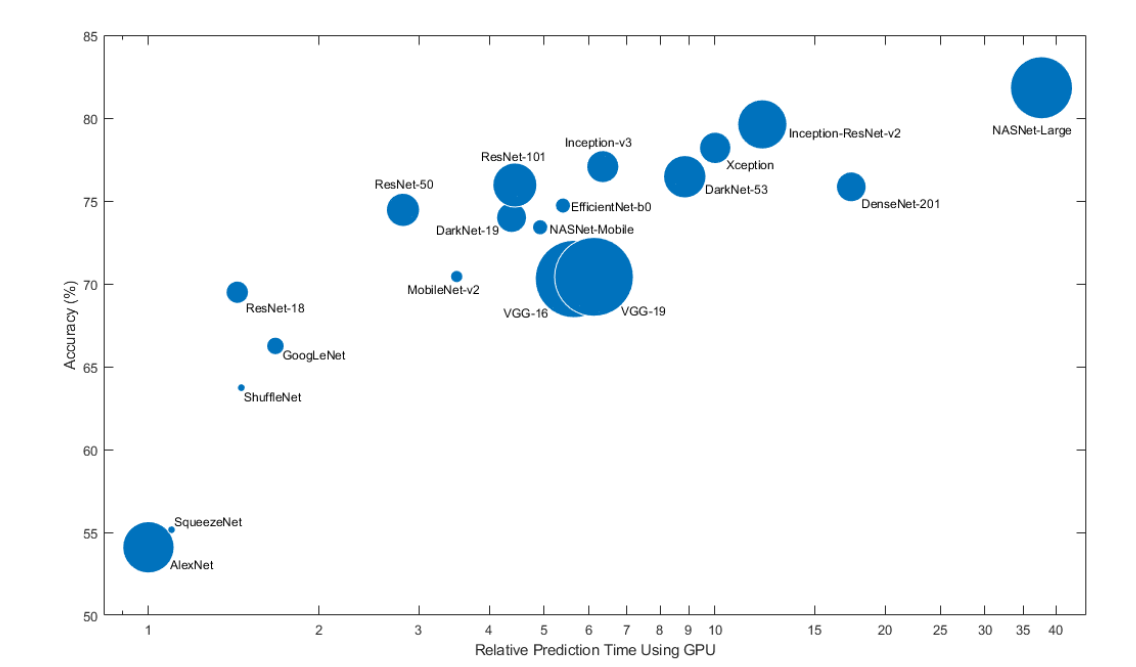
\includegraphics[width=1\textwidth]{Pre-trained_comparision.PNG}
    \caption{Compare Pretrained Neural Networks \cite{YOLo_NAS_Whitepaper_2022}}
    \label{fig: Pretrained Model Comparison}
\end{figure}

    % Umożliwia to również łatwą migrację do nowej wersji szablonu:
\section{Implemented object detection algorithm and Evolution of YOLO model}
This study aims to explore the performance of the YOLO-NAS and its variants on object detection tasks. Specifically, we evaluate the results of YOLO-NAS-S, YOLO-NAS-M, and YOLO-NAS-L on a dataset from the RoboFlow universe. RoboFlow provides various datasets that are structured accordingly, making it an ideal choice for this study. The dataset used in this study comprises 2481, 222, and 50 images for training, validation, and testing, respectively.

\begin{figure}[H]
  \begin{minipage}{0.48\textwidth}
    \centering
    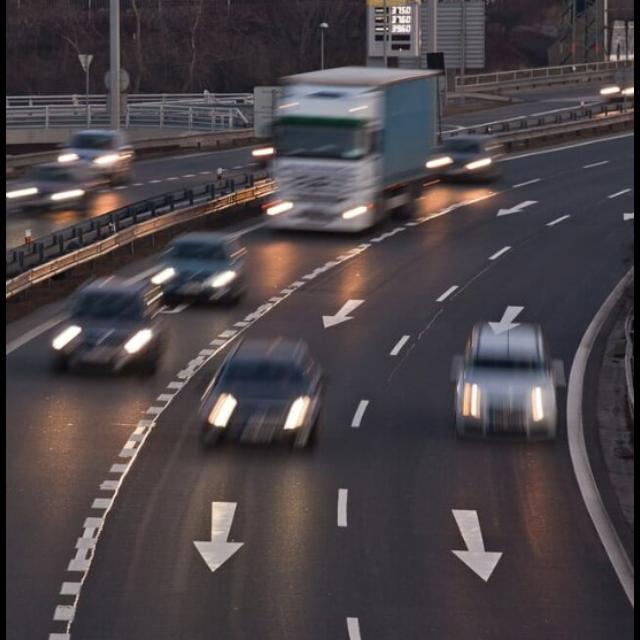
\includegraphics[width=\linewidth]{tex/img/train-1.jpg}
    \caption{Image-1: from Training dataset}
    \label{fig:tain-1}
  \end{minipage}%
  \begin{minipage}{0.5\textwidth}
    \centering
    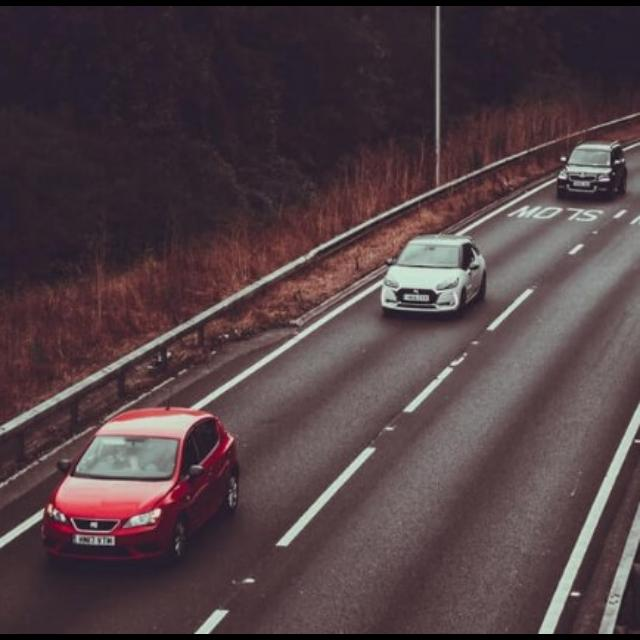
\includegraphics[width=\linewidth]{tex/img/train-2.jpg}
    \caption{Image-1: from Training dataset}
    \label{fig:train-2}
  \end{minipage}
  \begin{minipage}{0.5\textwidth}
    \centering
    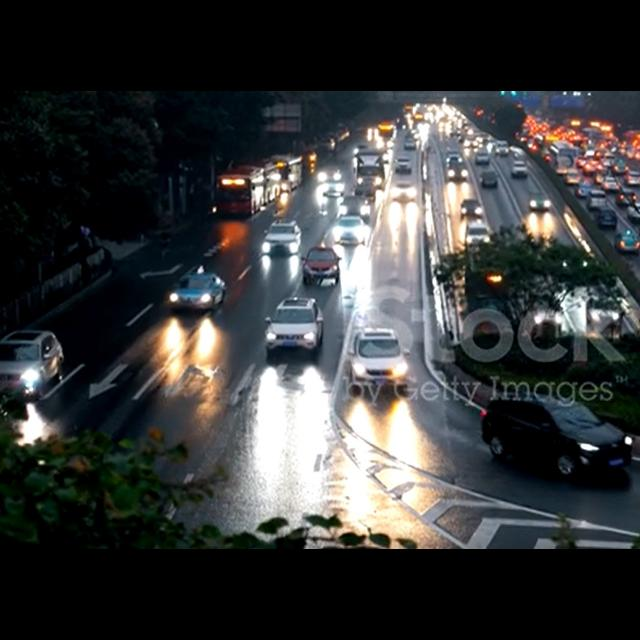
\includegraphics[width=\linewidth]{tex/img/valid-1.jpg}
    \caption{Image-1: from validation dataset}
    \label{fig:valid-1}
  \end{minipage}
    \begin{minipage}{0.5\textwidth}
    \centering
    \includegraphics[width=\linewidth]{tex/img/valid-2.jpg}
    \caption{Image-1: from validation dataset}
    \label{fig:valid-2}
  \end{minipage}
  \caption{Sample image from dataset I am going to fine-tune} 
\vspace{3mm}
  The image used to test the model is completely different from the dataset. Source: \href{https://www.istockphoto.com/pl/zdj%C4%99cie/wiele-samochod%C3%B3w-na-drodze-gm490081958-75026541}{iStock}
\end{figure}  
After fine-tuning and extensive training, we will test our models on a set of images obtained from iStock image stocks. The test dataset comprises a variety of images with different object sizes, orientations, and backgrounds. Some samples of our test dataset are provided in the figure below.

\begin{figure}[H]
  \begin{minipage}{0.48\textwidth}
    \centering
    \includegraphics[width=\linewidth]{tex/img/car-1.jpg}
    \caption{Car-1}
    \label{fig:YOLO-NASSM_vs_other_models}
  \end{minipage}%
  \begin{minipage}{0.5\textwidth}
    \centering
    \includegraphics[width=\linewidth]{tex/img/car-4.jpg}
    \caption{Car-2}
    \label{fig:YOLO-NAS_vs_other_models}
  \end{minipage}
  \begin{minipage}{0.5\textwidth}
    \centering
    \includegraphics[width=\linewidth]{tex/img/car-8.jpg}
    \caption{Car-3}
    \label{}
  \end{minipage}
    \begin{minipage}{0.5\textwidth}
    \centering
    \includegraphics[width=\linewidth]{tex/img/car-11.jpg}
    \caption{Car-4}
    \label{}
  \end{minipage}
  \caption{Sample image for testing the model after and before the training. This image is taken from Istock by Getty Images for testing the model only.} 
\vspace{3mm}
  The image used to test the model is completely different from the dataset. Source: \href{https://www.istockphoto.com/pl/zdj%C4%99cie/wiele-samochod%C3%B3w-na-drodze-gm490081958-75026541}{iStock}
\end{figure}  
To train and test my models, I will utilize Google Colab, which provides powerful computers specifically designed for deep learning purposes. The machine I used for our experiments had an NVIDIA Tesla T4 GPU with high RAM, enabling us to train and test our models efficiently. 

Our experiments involved training the models on the training dataset and evaluating their performance on the validation and test datasets. I will analyze the models' performance based on various metrics, including mean average precision (mAP), accuracy, and time taken for inference. I will also compare the performance of YOLO-NAS variants.

The results of our study will shed light on the performance of YOLO-NAS and its variants on object detection tasks and provide insights into their strengths and weaknesses. This study will contribute to the development of more efficient and accurate object detection models that can be applied in various domains, including self-driving cars, surveillance systems, and robotics.
\subsection{YOLO}
YOLO (You Only Look Once) is an object detection system for real-time object detection. Ross Girshick, Ali Farhadi, Santosh Divvala, and Joseph Redmon were the ones who first introduced it in 2016. YOLO is known for its high speed and accuracy. The system is designed to classify and detect multiple objects in an image using a single forward pass of the neural network.
Traditional object detection systems use a sliding window approach where they apply a classifier at each location and scale of the image. This process is computationally expensive and time-consuming. On the other hand, YOLO divides the input image into a grid of cells, and each cell is responsible for detecting an object. This approach reduces the number of bounding boxes that need to be processed and allows for real-time detection; this makes it suitable for a wide range of applications such as self-driving cars, surveillance systems, and robotics. Additionally, YOLO can detect objects at different scales and aspect ratios, making it robust to variations in object size and orientation. \cite{terven2023comprehensive} \cite{redmon2016you} 

\subsection{The Evolution of YOLO}
\begin{figure}[H]
    \centering
    \includegraphics[width=\textwidth]{evolution_of_YOLO.PNG}
    \caption{The evolution  of yolo [Source: \href{https://deci.ai/resources/webinar-open-source-llms-vs-apis/}{\textcolor{black}{Deci. ai webinar}}]}
    \label{fig:YOLO-Evolution}
\end{figure}
\begin{enumerate}
    \item \textbf{YOLO: } YOLO was introduced in 2016 for real-time object detection.
    Achieved a groundbreaking mAP of 63.4\% on the PASCAL VOC2007 dataset.
    YOLO's efficiency in one network pass. Localization error limitations due to object count, aspect ratios, and down-sampling. \cite{redmon2016you}\\
    \item \textbf{YOLOv2 Improvements: } YOLOv2 was introduced in 2017 with 9000+ categories.
    Improved with batch normalization, high-resolution classifiers, and anchor boxes.
    Joint training for classification and detection.\cite{sang2018improved}\\
    \item \textbf{YOLOv3 Advancements: } YOLOv3 (2018) achieved 60.6\% mAP on MS COCO, 2x faster than previous versions.
    Introduced logistic regression for objectness scores and anchor box priors. \cite{redmon2018yolov3}\\
    \item \textbf{YOLOv4 Global Impact: } YOLOv4 (2020) maintained YOLO's philosophy with bag-of-freebies and bag-of-specials. Enhanced accuracy with image adjustments like mosaic augmentation and DropBlock. \cite{gai2023detection}
    \item \textbf{YOLOv5 Speed and Efficiency: } YOLOv5 (2020) by Ultralytics in PyTorch achieved 50.7\% AP with user-friendly features. \cite{wu2021real}\\
    \item \textbf{YOLOX Anchor-Free Innovation: } YOLOX (July 2021) exceeded previous YOLO versions, anchor-free with center sampling. Employed MixUP, Mosaic augmentations for improved accuracy. \cite{ge2021yolox}\\
    \item \textbf{YOLOR Multi-Task Learning: } YOLOR (May 2021) focused on a unified network for multiple tasks.
    Applied multi-task learning for classification, detection, and pose estimation.\\

    \item \textbf{PP-YOLOv2: }  Upgrades include ResNet101, PAN, Mish Activation, increased input size, and modifications to IoU-aware branch. \cite{huang2021pp}\\
    \item \textbf{Scaled-YOLOv4 Flexibility: } Scaled-YOLOv4 (CVPR 2021) introduced scaling-up and scaling-down techniques. YOLOv4-tiny for low-end GPUs, YOLOv4-large for cloud GPUs. \cite{wang2021scaled}\\ 
    \item \textbf{PP-YOLO: } A YOLOv3-based model by Baidu, leveraging PaddlePaddle, introducing ten tricks for accuracy without sacrificing speed.\cite{long2020pp}\\
    \item \textbf{PP-YOLOE: } Evolved from PP-YOLOv2 with anchor-free architecture, new backbone, TAL, ET-head, and VFL/DFL. \cite{xu2022pp}\\
    \item \textbf{YOLOv6 Industrial Framework: } 
    YOLOv6 (September 2022) for industrial applications with anchor-free detection.
    YOLOv6-L achieved 52.5\% AP and 70\% AP50 at 50 FPS. \cite{li2022yolov6}, \cite{terven2023comprehensive}
    \item \textbf{YOLOv7 Speed and Accuracy: } YOLOv7 (July 2022) surpassed others in speed and accuracy.
    E-ELAN, model scaling, and "bag-of-freebies" approach for efficiency. \cite{wang2023yolov7}, \cite{terven2023comprehensive}\\
    \item \textbf{DAMO-YOLO Real-Time Improvements: } DAMO-YOLO (November 2022) by Alibaba for real-time object detection. 
    Introduced MAE-NAS, Efficient-RepGFPN, ZeroHead, and knowledge distillation. \cite{xu2022damo}\\
    \item \textbf{YOLOv8 :}
    YOLOv8 (January 2023) by Ultralytics with anchor-free prediction and faster NMS. Mosaic augmentation during training for improved accuracy.
    YOLOv8 offers five scaled versions: YOLOv8n (nano), YOLOv8s (small), YOLOv8m (medium), YOLOv8l (large), and YOLOv8x (extra\-large). YOLOv8x outperformed YOLOv5 on the MS COCO dataset with an impressive 53.9\% AP at 640 pixels and fast speed.\cite{yolov8}, \cite{terven2023comprehensive}
\end{enumerate}

\subsection{YOLO-NAS}
YOLO-NAS is a cutting-edge object detection model created using Deci's Neural Architecture Search technology, AutoNAC™. It offers unmatched real-time object detection capabilities and production-ready performance, surpassing other models such as YOLOv5, YOLOv6, YOLOv7, and YOLOv8.

The YOLO-NAS model undergoes a multi-phase training process that involves pre-training on Objects365, COCO Pseudo-Labeled data, Knowledge Distillation (KD), and Distribution-Focal-Loss (DFL).

During the pre-training phase, the model is trained on Objects365, a comprehensive dataset that consists of 2 million images and 365 categories. Depending on the model variant, this process can take 25-40 epochs, as each epoch requires 50-80 minutes on 8 NVIDIA RTX GPUs. 

The COCO dataset offers an additional 123,000 images without labels. These images are utilized to create pseudo-labeled data. First, an accurate model is trained on COCO to label these images. Then, the labeled images are used to train our model alongside the 118,000 train images.

The YOLO-NAS architecture incorporates Knowledge Distillation (KD) and Distribution Focal Loss (DFL) techniques to improve its training process. Furthermore, the YOLO-NAS training procedure employs various datasets, including both labeled and unlabeled data, as well as supervised and unsupervised training methods.\cite{YOLO-NAS}, \cite{terven2023comprehensive}
\begin{figure}[H]
    \centering
    \includegraphics[width=0.8\textwidth]{YOLO-NAS-Training.PNG}
    \caption{An overview of the YOLO-NAS training process \cite{richmond_yolo-nas}}
    \label{fig:enter-label}
\end{figure}


\subsubsection{Architectural Features of YOLO-NAS} \vspace{0mm}It is considered one of the most efficient object detection algorithms due to its unique architecture, which is designed to minimize the computational cost of the algorithm while maintaining high accuracy.
\begin{enumerate}
    \item \textbf{Quantization Aware Blocks and Selective Quantization: } 
        \begin{itemize}
            \item \textbf{Hybrid Quantization Method: } YOLO-NAS uses a mixed quantization method that includes both Quantization-Specific Parameters (QSP) and Quantization-Centric Initialization (QCI) blocks. These leverage re-parameterization and 8-bit quantization, inspired by Chu et al.'s methodology.
            \item  \textbf{Selective Quantization:} The model strategically quantizes specific parts rather than uniformly affecting all layers. This selective quantization balances accuracy and latency, addressing information loss, a common issue in standard quantization techniques.
                \item \textbf{Layer Selection Algorithm:} YOLO-NAS utilizes a sophisticated layer selection algorithm to decide which layers to quantize. It evaluates the impact of each layer on accuracy and latency, carefully considering the implications of toggling between 8-bit and 16-bit quantization.
                \item \textbf{Performance in Limited Resources:} Uniquely designed for environments with limited resources, YOLO-NAS ensures superior performance. Its optimized approach to quantization preserves accuracy while being efficient, striking a crucial balance for advanced object detection tasks.
        \end{itemize}
    \item \textbf{Detection Head: } A standout feature of YOLO-NAS is its detection head design, which predicts a distribution probability for size regression. This approach is particularly useful in scenarios where the object sizes vary significantly. YOLO-NAS is an object detection model that predicts a range of possible sizes instead of a single fixed size. This unique approach improves its accuracy in detecting objects of varying scales. In addition, YOLO-NAS uses a probabilistic approach to size regression which makes it suitable for knowledge distillation. This means that it facilitates a more nuanced transfer of knowledge from a complex, high-capacity teacher model to a simpler, more efficient student model. All these features make YOLO-NAS a practical choice for diverse applications.
    \item \textbf{Neck: } The YOLO-NAS network has a highly advanced pyramid-attention neck that combines both top-down and bottom-up information flows. 
    \begin{figure}[H]
        \centering
        \includegraphics[width=\textwidth]{yolo-nas_neck.PNG}
        \caption{Neck Design}
        \label{fig:Neck}
    \end{figure}
    This design element assists the network in effectively capturing and utilizing multi-scale information. In this pyramid-attention structure, the top-down pathway captures high-level semantic information, while the bottom-up pathway focuses on smaller details. The attention mechanism in this pyramid structure ensures that the network focuses on the most relevant features at different scales, which improves its ability to detect objects with varying sizes and complexities. 
    \item \textbf{Backbone: } 
The backbone of YOLO-NAS is a significant component of its architecture, which is the result of an advanced Network Architecture Search (NAS) process. The process utilizes Deci's proprietary NAS technology, AutoNAC, to tailor the network structure for object detection tasks with unparalleled precision. This innovative approach ensures that the network structure meets the specific demands of the tasks at hand.
\begin{itemize}
    \item \textbf{quantization-aware RepVGG: } During the NAS process, they have incorporated quantization-aware RepVGG blocks into the model architecture, ensuring that our model architecture would be compatible with Post-Training Quantization (PTQ).\\
    \item \textbf{Spatial Pyramid Pooling (SPP): } YOLO-NAS backbone has Spatial Pyramid Pooling (SPP)  at the end to capture global context; it is a pooling layer that removes the fixed-size constraint of the network, i.e., a CNN does not necessitate a fixed or predetermined picture size input. Placing SPP at the end of the YOLO-NAS backbone allows the model to capture global context information, which is crucial for understanding the overall context of the scene. This can be beneficial for detecting objects that may span a larger region in the image.\cite{YOLO-NAS}
\end{itemize}

\href{https://deci.ai/blog/yolo-nas-object-detection-foundation-model/}{Source}

\begin{figure}[H]
    \centering
    \includegraphics[width=\textwidth]{Yolo-BackBone.PNG}
    \caption{Backbone Structure}
    \label{fig:BackBone}
\end{figure}

AutoNAC plays a crucial role in the NAS process by determining the optimal sizes and structures of different stages in the YOLO-NAS backbone. This involves configuring the block type, number of blocks, and channels in each stage meticulously. Consequently, AutoNAC guarantees that every part of the backbone is meticulously optimized for its specific function. The NAS-generated backbone is not just a result of automated design but also of intelligent decision-making that considers various factors such as computational efficiency, accuracy, and speed. This ensures that the backbone contributes effectively to the overall robustness and adaptability of YOLO-NAS. These advancements lead to a superior architecture with exceptional object detection capabilities and outstanding performance compared to its predecessors.
\end{enumerate} 

\subsubsection{Automated Neural Architecture Construction (AutoNAC) engine}
Deci created the optimization engine AutoNAC, which Deci-AI uses. This engine applies Neural Architecture Search (NAS) to enhance the architecture of a deep learning model. The main goal is to improve the performance of the model when it is executed on specific hardware while maintaining or even improving its accuracy. The AutoNAC engine is hardware aware, data-aware and considers all the components in the inference stack, including compilers and quantization. \\
AutoNAC is essentially a NAS engine takes three components as inputs. \cite{yolo-nas-webinar}
\begin{itemize}
    \item \textbf{Task: } Firstly, we need to decide which model to build, such as an object detection model.\\
    \item \textbf{Data characteristics: } Deci Group requires the NAS Engine to be data-aware or capable of understanding the characteristics of the data so that it can create a model that is well-suited for the task at hand. For instance, if the objective is to detect small objects, the model would likely be different from that required for detecting large objects, as the receptive fields would differ. \\
    \item \textbf{Inference environment and Hardware: } When it comes to computer vision on edge, the priority is to achieve real-time performance or improve some level of latency or throughput while being hardware-aware, compilation-aware, and quantization-aware. To achieve this, we need to consider factors such as model size, latency, and throughput. Decis Group's goal is to optimize these factors as part of the Neural Architecture Search (NAS) process. Manually finding the optimal architecture for object detection models can be a laborious and inefficient process. To address this issue, Deci utilized AutoNAC, a tool that uses neural design space incorporating state-of-the-art (SOTA) architectural design principles and Deci's novel neural elements, to discover novel object detection models. These models were optimized to minimize inference latency computed over NVIDIA's T4 cloud GPU, which is a widely used computing device. We achieve this by feeding all three inputs into the AutoNAC engine, which generates a new architecture.
\end{itemize}
 
\begin{figure}[H]
    \centering
    \includegraphics[width=\textwidth]{autoNAC_Engine.PNG}
    \caption{Deci's AutoNAC Engine; \\
    Hardware-Aware Neural Architecture Search for DL Inference Efficiency \cite{YOLo_NAS_Whitepaper_2022}\cite{yolo-nas-v8-sota}}
    \label{fig:AutoNAC Engine}
\end{figure}

\subsubsection{Under the hood View of Auto-NAC}
NAS algorithms can methodically search through the vast space of potential architectures, effectively locating novel and optimized configurations that human intuition might miss. By automating the process, these algorithms can quickly evaluate and compare an unimaginably large number of candidate architectures. They will eventually find a solution that strikes the best balance between accuracy, speed, and complexity. The NAS engine will be used when we already have data and want to build a model.
it takes all three inputs mentioned above, and the search space is automatically created under the hood, considering all the possibilities of neural architecture as an input. For example, optimal sizes, block types, number of blocks, and channel counts in every stage. \cite{yolo-nas-webinar} \cite{YOLo_NAS_Whitepaper_2022}
\begin{figure}[H]
    \centering
    \includegraphics[width=\textwidth]{AUTONACENGINE_Underthe hood.PNG}
    \caption{AutoNAC Engine Search Space \cite{yolo-nas-webinar}}
    \label{fig:autonac_under_the_hood}
\end{figure}
Finally, AutoNAC Engine explores and maps the efficiency frontier, searching for an architecture that best balances latency vs. throughput. Deci Group samples three points of this frontier to create the YOLO-NASS, YOLO-NASM, and YOLO-NASL architectures.
\subsubsection{How to find the best architecture out of the search space}
while the search space has trillions of candidate architectures, the task of identifying the optimal architecture becomes increasingly challenging. Within the realm of Deci, the selection of the most suitable candidate from the numerous models within the extensive search space is guided by two distinct evaluation criteria. \cite{yolo-nas-webinar}
\begin{enumerate}
    \item \textbf{Bench Marking: } Understanding how the model will behave on the expected hardware or using the techniques of Latency Vs. throughput for the candidate architecture. \\
    \item \textbf{Accuracy Potential Predictions: } The fundamental selection methodology of best candidate out of the search space involves the provision of an AI model, designated to assess the accuracy or potential accuracy of neural network models. Leveraging principles from neural architecture search, YOLO-NAS systematically navigates the expansive design space of possible neural network configurations, employing optimization algorithms to identify architectures anticipated to yield high accuracy on the specified object detection task.
\end{enumerate}
 \begin{figure}[H]
     \centering
     \includegraphics[width=\textwidth]{Yolo_nas.png}
     \caption{\textbf{YOLO-NAS Architecture \cite{YOLO-NAS}. The architecture is found automatically via a Neural Architecture Search(NAS) system called AutoNAC to balance latency vs. throughput. They generated three architectures called YOLO-NASS(small), YOLO-NASM(medium), and YOLO-NASL(large), varying the depth and the position of the QSP and QCI blocks \cite{YOLO-NAS}}}
     \label{fig:YOLO-NAS Architecture.}
\end{figure}


\subsubsection{Fine-tuning of the selected model On custom data set}
Fine-tuning refers to the process of making minor adjustments to achieve the desired output or performance. In deep learning, pre-existing trained neural networks can be used to program another deep learning algorithm from the same domain by using their weights. These weights are responsible for connecting each neuron in one layer to every neuron in the next layer of the neural network. Fine-tuning can be used to speed up the training process and overcome a small dataset as it already contains vital information from the pre-existing deep learning algorithm. The YOLO-NAS architecture and pre-trained weights are an excellent starting point for fine-tuning downstream tasks and define a new frontier in low-latency inference. When fine-tuning, using strong pre-trained weights often leads to higher model accuracy on new datasets. YOLO-NAS was trained on the RoboFlow100 dataset, which is a collection of 100 datasets from diverse domains, to demonstrate its ability to handle complex object detection tasks. The RF100 dataset is a benchmark for existing YOLO models, enabling us to compare YOLO-NAS's performance against them and showcase its advantages.\cite{YOLO-NAS}
\begin{figure}[H]
    \centering
    \includegraphics[width=0.8\textwidth]{YOLO-NAS_RF100_benchmark.PNG}
    \caption{Examples of annotated images in the RF100 benchmark \cite{YOLO-NAS}}
    \label{fig:YOLO-NAS_RF100_benchmark}
\end{figure}
The following hyperparameters ensure a robust and consistent training process, allowing for a fair comparison of the model’s performance across different datasets.\\
Deci followed the RF100 repository’s training protocol to ensure a fair comparison.\\
The model was trained for 100 epochs on a single T4 GPU with 16GB of VRAM, using consistent settings across all datasets.\cite{YOLO-NAS}, \cite{yolo-nas-vs-yolov8}
\begin{itemize}
    \item Learning rate: a learning rate of 5e-4 is used, while for the Medium version, the learning rate is set to 4e-4.
    \item Weight decay: 1e-4 (excluding bias and BatchNorm layers)
    \item Exponential moving average (EMA) with a decay factor of 0.99
    \item Batch size: 16
    \item Image resolution: 640×640
\end{itemize}


\begin{figure}[H]
  \begin{minipage}{0.48\textwidth}
    \centering
    \includegraphics[width=\linewidth]{YOLO-NASSM_vs_other_models.PNG}
    \caption{Average mAP on Roboflow-100 \\for YOLO-NAS vs other models.}
    \label{fig:YOLO-NASSM_vs_other_models}
  \end{minipage}%
  \begin{minipage}{0.5\textwidth}
    \centering
    \includegraphics[width=\linewidth]{YOLO-NAS_vs_other_models.PNG}
    \caption{Per category mAP score for YOLO-NAS vs other models.
    Note: For Yolo vV5/v7/v8}
    \label{fig:YOLO-NAS_vs_other_models}
  \end{minipage}
  \caption{Average mAP and Per category mAP score for YOLO-NAS vs other models. \cite{YOLO-NAS}}
\end{figure}
Figure \ref{fig:YOLO-NASSM_vs_other_models} are the results obtained by focusing on the “Small” and “Medium” YOLO-NAS variants, and figure: \ref{fig:YOLO-NAS_vs_other_models} is a per-category breakdown of YOLO-NAS’s performance on the RF-100 dataset, compared to the performance of v5/v7/v8 models. \cite{YOLO-NAS}, \cite{yolo-nas-v8-sota}
\subsubsection{Object Detection Evaluation Metrics}
Object detection metrics are measurements that are used to assess the effectiveness of object detection algorithms. These metrics are essential in determining the accuracy and efficiency of object detection models, as they provide insights into the model's ability to identify and locate objects within images. Furthermore, they help in identifying false positives and false negatives. This information is critical in evaluating and improving the model's performance. There are many evaluation metrics that are applicable across different object detection algorithms, including the YOLO-NAS model. \cite{metrics}

\begin{itemize}
    \item \textbf{Intersection over Union (IoU):} Intersection over Union (IoU) is a fundamental measure that quantifies the overlap between a predicted bounding box and a ground truth bounding box. It plays a crucial role in evaluating the accuracy of object localization.
    \item \textbf{Average Precision (AP):} AP calculates the area under the precision-recall curve, producing a single value that encompasses precision and recall performance.
    \item \textbf{Mean Average Precision (mAP):} mAP calculates the average AP values across multiple object classes, making it useful in multi-class object detection scenarios for comprehensive model performance evaluation.
    \item \textbf{Precision and Recall:} Precision and Recall are two important metrics used to evaluate the performance of classification models. Precision measures the percentage of true positives among all positive predictions, indicating the model's ability to avoid false positives. Recall, on the other hand, calculates the percentage of true positives among all actual positives, indicating the model's ability to detect all instances of a class. These metrics are often used together to provide a more complete picture of a model's performance.
    \item F1 Score: The F1 Score is a measure of a model's performance that takes into account both precision and recall. It provides a balanced assessment while considering false positives and negatives.
\end{itemize}

\subsubsection{Benefits of YOLO-NAS over other models}
\textbf{Optimized Efficiency: }\\
YOLO-NAS is an advanced model that has been designed to achieve an optimal balance between accuracy and speed, making it more efficient than other human-designed models. This optimization is essential for real-time object detection applications as it enhances inference speeds and improves resource utilization. YOLO-NAS outperforms other models in terms of efficiency, making it the go-to choice for those who demand high-performance object detection capabilities." \\
\textbf{Adaptability to Diverse Tasks and Hardware: }\\
The architecture of YOLO-NAS allows it to adapt to various object detection tasks, including complex scenarios and hardware. Its versatility makes it a valuable tool across a wide range of applications.\\
\textbf{Training on Prominent Datasets: }\\
The architecture of YOLO-NAS allows it to adapt to various object detection tasks, including complex scenarios and hardware. Its versatility makes it a valuable tool across a wide range of applications.\\
\textbf{Detection and Localization Accuracy: }\\
The YOLO-NAS architecture is a specialized object detection model that addresses the challenges associated with detecting small or intricate objects. Its heightened detection capabilities and improved accuracy in pinpointing precise locations make it a superior choice for a diverse range of applications, particularly those where identifying small or elusive objects is crucial. In contrast, the YOLOv8 object detection model, while impressive, is limited in its ability to detect small objects accurately and localize them with precision. Despite its proficiency in various scenarios, YOLOv8 falls short when compared to the specialized capabilities of YOLO-NAS in handling the challenges posed by diminutive objects. \cite{yolo-nas-vs-yolov8}
\begin{figure}[H]
    \centering
    \includegraphics[width=0.7\textwidth]{YOLO-V8_vs_YOLO-NAS.PNG}
    \caption{Performance evaluation on YOLO-V8 vs. YOLO-NAS (\href{https://www.youtube.com/watch?v=uPgE8G4CGF4} Image Source: {\textcolor{black}{Youtube}})}
    \label{Yolo-V8_vs_YOLO-NAS}
\end{figure}


\subsubsection{Data set}
\label{datset}
The "Smart City Cars Detection Computer Vision Project" stands as a meticulously curated dataset within the Roboflow Universe, purposefully designed for object detection, with a specific emphasis on vehicular recognition. Encompassing various vehicle types, including buses, cars, motorbikes, and trucks this dataset plays a crucial role in advancing computer vision applications.
Regarding key attributes, the project adopts an object detection framework with distinct classes such as bus, car, motorbike, and truck. The dataset comprises 2753 after preprocessing applied from 1099 original images, with data allocation distributed as 90\texttt{\%} for training, 8\texttt{\%}for validation, and 2\texttt{\%} for testing.

During preprocessing, the image is resized to fit within a 640x640 frame, with black edges if necessary. Augmentations include rotating between -15° and +15°, shearing horizontally and vertically by ±15°, adjusting hue between -25° and +25°, saturating between -40\texttt{\%} and +40\texttt{\%}, applying blur up to 4 pixels, introducing noise up to 3\texttt{\%} of pixels, and utilizing mosaic augmentation. For bounding boxes, cropping ranges from 0\texttt{\%} minimum zoom to 20\texttt{\%} maximum zoom, and brightness is adjusted between -30\texttt{\%} and +30\texttt{\%}. The model generates three outputs per training example.

This dataset holds substantial utilitarian significance across various domains. It facilitates real-time traffic monitoring and analysis, contributing to Employing the Smart City Cars Detection model to process live video feeds of traffic, recognize various vehicle types and their numbers, and adjust traffic light timings dynamically. This optimization aims to reduce congestion and enhance the overall traffic flow within a smart city environment.   

Additionally, it Utilizes the Smart City Cars Detection model for monitoring parking areas, distinguishing between different vehicle classes occupying spaces (cars, trucks, buses, motorbikes), and offers drivers real-time updates on parking space availability through smart parking applications, Integrate findings from the Smart City Cars Detection model to analyze the distribution of diverse vehicle types in specific locations or across the entire city. This information aids city planners in devising focused infrastructure development plans, such as dedicated bus lanes, motorcycle parking, or optimized truck routes, Input the Smart City Cars Detection model data into machine learning algorithms for the autonomous generation of precise forecasts regarding future traffic patterns. This includes predicting peak hours and identifying locations prone to congestion, enabling proactive measures to be implemented. Mostly, Employ the Smart City Cars Detection model to observe bus utilization within a city, recognizing both bus occupancy and frequency. Utilize this information to enhance public transportation routes, determining whether additional buses or different types of public transport are required for more efficient service to the population.

The "Smart City Cars Detection Image Dataset" dataset epitomizes substantive potential across domains, ranging from traffic management and security to autonomous vehicles, fleet management, and traffic accident analysis.\cite{p4p-cars_dataset}

 % zazwyczaj wystarczy podmienić plik src/wut-thesis.cls
\section{Object detection Implementations and fine-tuning on custom dataset}

\begin{enumerate}
    \item \textbf{Environment Setup: } Google CoLab is a free research environment provided by $Google^{Tm}$. Using Google Colab for training deep learning models, including YOLO-NAS, provides you with access to free GPU resources. Before we start training, we need to prepare our Python environment and start by installing the required packages.
    The YOLO-NAS model is distributed using a \boxed{\textcolor{black}{super-gradients}}  package. In addition, we will install \boxed{roboflow} and \boxed{supervision}. Roboflow will enable us to download the dataset from the Roboflow Universe, while Supervision will allow us to visualize the outcomes of our training. We use \boxed{\texttt{!pip install}} to install the required package. \cite{supergradients}
    
    \begin{lstlisting}[language=Python, caption=Installing the required package]
    !pip install super-gradients
    !pip install roboflow
    !pip install supervision
        
    \end{lstlisting}
    \item \textbf{Load YOLO-NAS Model}
    I have automated the selection of the model. To support the open-source community, the Deci group has released the capability to fine-tune YOLO-NAS models on the RF100 dataset within the SuperGradients library. To perform inference using the pre-trained model, we first need to choose the model size. YOLO-NAS offers three different model sizes:  \verb|yolo_nas_s|, \verb|yolo_nas_m|, and \verb|yolo_nas_l|.
    \begin{lstlisting}[language=Python, caption=importing models from the supergradients][H]
    #[Original Version]
    from super_gradients.training import models
    
    model = models.get(yolo_nas_l, pretrained_weights="coco").to(DEVICE)
    
    #[The Modified Version]
    import torch #gives us access to some helpful neural network things,
    such as various neural network layer types

    DEVICE = 'cuda' if torch.cuda.is_available() else "cpu"  #Check if
    GPU is available
    
    MODEL_ARCH_OPTIONS = ['yolo_nas_l', 'yolo_nas_m', 'yolo_nas_s']
    
    # Display options to the user
    print("Choose a model architecture:")
    for i, MODEL_ARCH in enumerate(MODEL_ARCH_OPTIONS, start=1):
        print(f"{i}. {MODEL_ARCH}")
    
    # Take input from the user
    while True:
        try:
            user_input = int(input("Enter your choice number: "))
            if 1 <= user_input <= len(MODEL_ARCH_OPTIONS):
                selected_model_arch = MODEL_ARCH_OPTIONS[user_input - 1]
                print(f"Selected Model Architecture: {selected_model_arch}")
                break
            else:
                print("Invalid input. Please enter a valid number.")
        except ValueError:
            print("Invalid input. Please enter a valid number.")
    




    \end{lstlisting}
    \item \textbf{Dataset Download and Directory Structure: }
   To perform model fine-tuning, the acquisition of pertinent data is imperative. The requisite dataset structure for this endeavor adheres to the YOLO format. I am utilizing a dataset from the Roboflow universe, encompassing a vast repository of over 100,000 open-source computer vision datasets. Significantly, the dataset obtained from Roboflow is inherently organized to align with the prescribed folder structure mandated by YOLO standards.

    \begin{lstlisting}[caption=Dataset folder structure YOLO format][style=custom,language=sh]
    /directory_to_your_dataset
    |-- train
    |   |-- images
    |   |   |-- image1.jpg
    |   |   |-- image2.jpg
    |   |   |-- ...
    |   |-- labels
    |       |-- image1.txt
    |       |-- image2.txt
    |       |-- ...
    |-- valid
    |   |-- images
    |   |-- labels
    |-- test
    |   |-- images
    |   |-- labels
    \end{lstlisting}
    Each image file should have a corresponding label file in the YOLO format, which contains one line per object in the image. Each line should have the following format:
    \texttt{<class\_id> <x\_center> <y\_center> <width> <height>}
    
    where \verb|<class_id>| is an integer representing the class of the object, and 
    \texttt{<x\_center>, <y\_center>, <width>, and <height>}
    are the normalized coordinates of the bounding box.
   In the process of importing data from the Roboflow universe, the inclusion of a data.yaml file is an automated or default feature. This file serves as a dictionary, encapsulating the names of classes associated with the imported data. 
    The order of the class names should match the \texttt{<class\_id>} in the label files.
    \item \textbf{Dataset Parameters for Training YOLO NAS}
    After preparing your data, you need to create a Python dictionary that outlines the key elements of your dataset’s structure, as such: 
    \begin{lstlisting}[language=Python]
        dataset_params = {
        'data_dir': LOCATION,
        'train_images_dir': 'train/images',
        'train_labels_dir': 'train/labels',
        'val_images_dir': 'valid/images',
        'val_labels_dir': 'valid/labels',
        'test_images_dir': 'test/images',
        'test_labels_dir': 'test/labels',
        'classes': CLASSES
    }
    \end{lstlisting}
    Using the \texttt{dataset\_params} we can easily create the datasets in the required format later on,   Where LOCATION is the path to the main directory where your dataset resides, and CLASSES is the list of class names you created earlier. It's important to specify the number of training epochs, batch size, and data processing workers.
    \begin{lstlisting}[language=Python]
        EPOCHS = 60,
        BATCH_SIZE = 16,
        WORKERS = 8 
    \end{lstlisting}

     
    \item \textbf{Setting-up dataloaders: }  SuperGradients provides ready-to-use dataloaders for the datasets it supports. Import the required modules for SuperGradients dataloaders.\cite{supergradients}
    \begin{lstlisting}[language=Python, caption=Setting-Up Dataloaders]
    from super_gradients.training import dataloaders
    from super_gradients.training.dataloaders import
    (coco_detection_yolo_format_train, coco_detection_yolo_format_val) 
    \end{lstlisting}
     For training, validation, and testing sets, create data loaders with a given batch size and workers Below we use \texttt{batch\_size}=16 and \texttt{num\_workers}=2. Note that we use \verb|coco_detection_yolo_format_val| for training and testing data to instantiate the dataloader.  
     \begin{lstlisting}[language=Python, caption=Setting-Up Dataloaders]
        from IPython.display import clear_output 
        train_data = coco_detection_yolo_format_train(
            dataset_params={
                'data_dir': dataset_params['data_dir'],
                'images_dir': dataset_params['train_images_dir'],
                'labels_dir': dataset_params['train_labels_dir'],
                'classes': dataset_params['classes']
            },
            dataloader_params={
                'batch_size': BATCH_SIZE,
                'num_workers': 2
            }
        )
        
        val_data = coco_detection_yolo_format_val(
            dataset_params={
                'data_dir': dataset_params['data_dir'],
                'images_dir': dataset_params['val_images_dir'],
                'labels_dir': dataset_params['val_labels_dir'],
                'classes': dataset_params['classes']
            },
            dataloader_params={
                'batch_size': BATCH_SIZE,
                'num_workers': 2
            }
        )
        
        test_data = coco_detection_yolo_format_val(
            dataset_params={
                'data_dir': dataset_params['data_dir'],
                'images_dir': dataset_params['test_images_dir'],
                'labels_dir': dataset_params['test_labels_dir'],
                'classes': dataset_params['classes']
            },
            dataloader_params={
                'batch_size': BATCH_SIZE,
                'num_workers': 2
            }
        )
        clear_output()
     \end{lstlisting}
     \item \textbf{Model Instantiation for Fine-Tuning}
     Choose the YOLO-NAS variant (e.g., \texttt{yolo\_nas\_l}) and launch the model, tailoring the number of classes to your dataset.
     \begin{lstlisting}
        from super_gradients.training import models
        model = models.get(selected_model_arch , num_classes=len(dataset_params
        ['classes']), pretrained_weights="coco")
     \end{lstlisting}
    \item \textbf{Training Parameters and Metrics: } While utilizing SuperGradients, define your training parameters thoughtfully because they will affect your training process and significantly impact your model's performance. To help you get started, here's a brief overview of the most crucial parameters and some advanced features you should consider. \cite{supergradients}\\
    
    \textbf{Essential Training Parameters}\\
    \begin{itemize}
        \item \textbf{\texttt{max\_epochs}}: Tells the upper limit for the number of training cycles.\\
        \item \textbf{loss: } Select an appropriate loss function for your model and dataset. \\
        \item \textbf{optimizer: } Choose an optimizer and modify it if needed using \texttt{optimizer\_params}.\\
        \item \textbf{\texttt{train\_metrics\_list}/\texttt{valid\_metrics\_list}: } Specify metrics for evaluating training and validation performance. These are implemented as \href{https://lightning.ai/docs/torchmetrics/stable/}{Torchmetric} objects. \\
        \item \textbf{\texttt{metric\_to\_watch}: } Select a primary metric to determine checkpoint saving. \\
    \end{itemize} 
    
    \textbf{Advanced Features and Integrations}\\
    \begin{itemize}
        \item \textbf{Monitoring Tools: } There a lot of monitoring tools like Weights, Tensorboard,   ClearML, Biases, or for tracking training progress. Custom integrations can be achieved using Base SGLogger.
        \item \textbf{Enhancing the Training : } there are so many features in supergradients SuperGradients like Exponential Moving Average(EMA), Zero Weight Decay on Bias and Batch Normalization, Weight Averaging, Batch Accumulation, and Precise BatchNorm for optimized training.
        \item \textbf{Custom Metrics: } SuperGradients is customizable allows create custom metrics.
    \end{itemize}
    
    \textbf{Loss and Detection Metrics Setup: }\\
   Setup Loss and Detection Metrics: 
 correct number of classes for functions like PPYoloELoss and DetectionMetrics\_050 to align with dataset specifics.
    
    \begin{lstlisting}[language=Python]
        from super_gradients.training.losses import PPYoloELoss
        from super_gradients.training.metrics import DetectionMetrics_050
        from super_gradients.training.models.detection_models.pp_yolo_e 
         import PPYoloEPostPredictionCallback
        
        
        train_params = {
           # ENABLING SILENT MODE
           'silent_mode': True,
           "average_best_models":True,
           "warmup_mode": "linear_epoch_step",
           "warmup_initial_lr": 1e-6,
           "lr_warmup_epochs": 3,
           "initial_lr": 5e-4,
           "lr_mode": "cosine",
           "cosine_final_lr_ratio": 0.1,
           "optimizer": "Adam",
           "optimizer_params": {"weight_decay": 0.0001},
           "zero_weight_decay_on_bias_and_bn": True,
           "ema": True,
           "ema_params": {"decay": 0.9, "decay_type": "threshold"},
           # ONLY TRAINING FOR 10 EPOCHS FOR THIS EXAMPLE NOTEBOOK
           "max_epochs": 10,
           "mixed_precision": True,
           "loss": PPYoloELoss(
               use_static_assigner=False,
               # NOTE: num_classes needs to be defined here
               num_classes=len(dataset_params['classes']),
               reg_max=16
           ),
           "valid_metrics_list": [
               DetectionMetrics_050(
                   score_thres=0.1,
                   top_k_predictions=300,
                   # NOTE: num_classes needs to be defined here
                   num_cls=len(dataset_params['classes']),
                   normalize_targets=True,
                   post_prediction_callback=PPYoloEPostPredictionCallback(
                       score_threshold=0.01,
                       nms_top_k=1000,
                       max_predictions=300,
                       nms_threshold=0.7
                   )
               )
           ],
           "metric_to_watch": 'mAP@0.50'
        }
    \end{lstlisting}
    \item \textbf{Instantiate the training: }
    \begin{lstlisting}[language=Python, caption=Commencing the Training, escapeinside=``]
        trainer.train(model=model, training_params=train_params,
        train_loader=train_data, valid_loader=val_data)
    \end{lstlisting}
    \item \textbf{ Fetching the Best(Optimal) Model after Training: } Following intensive training, wherein the model underwent rigorous learning iterations, we are now focused on retrieving the best-trained model. This phase involves selecting the most refined and proficient version of the model, one that has successfully absorbed and generalized patterns from the training data. The goal is to identify the model that exhibits superior performance, ensuring its readiness for deployment in real-world scenarios. This meticulous retrieval process is crucial for obtaining a highly capable and reliable model that aligns with the desired objectives and expectations. In SuperGradients, this involves selecting the most effective set of weights from your training runs.\\
    \textbf{Using Checkpoint Averaging}
    \begin{addmargin}[8mm]{0mm}
    \footnotesize
    \begin{lstlisting}[language=Python, caption=Load trained model][H]
    from super_gradients.training import models

    # Path to the best weight checkpoint
    averaged_checkpoint_path = 'checkpoints/Experiment_name/average_model.pth'
    
    # Retrieve the model with averaged weights
    best_model = models.get(
            selected_model_arch,
            num_classes=len(dataset_params['classes']),
            checkpoint_path=f"{CHECKPOINT_DIR}/{EXPERIMENT_NAME}/ckpt_best.pth"
    ).to(DEVICE)
    \end{lstlisting}
    \end{addmargin}
    \item \textbf{Evaluate trained model}
    \begin{addmargin}[8mm]{0mm}
    \begin{lstlisting}[language=Python, caption=Model Evaluation on Test Data][H]
        trainer.test(
            model=best_model,
            test_loader=test_data,
            test_metrics_list=DetectionMetrics_050(
                score_thres=0.1,
                top_k_predictions=300,
                num_cls=len(dataset_params['classes']),
                normalize_targets=True,
                post_prediction_callback=PPYoloEPostPredictionCallback(
                    score_threshold=0.01,
                    nms_top_k=1000,
                    max_predictions=300,
                    nms_threshold=0.7
                )
            )
        )
    \end{lstlisting}
    \end{addmargin}
    \item \textbf{Model Evaluation on Test Data: } Evaluating a model on test data is a pivotal phase within the machine learning workflow, gauging the effectiveness of a trained model on new data. The primary objective is to ascertain the model's generalization capability for novel, unseen instances. This section outlines the prevalent metrics and procedures employed in assessing a model using test data.
\begin{addmargin}[8mm]{0mm} 
\footnotesize
\begin{lstlisting}[language=Python, caption=Inference with trained model]
Images ='Path_to_image'
images_predications = best_model.predict(Images, iou=0.5, conf=0.5).show()   
\end{lstlisting}
\end{addmargin}


    

\end{enumerate}
\section{Result and discussion}
The YOLO-NAS has YOLO-NAS-L, YOLO-NAS-M, and YOLO-NAS-S variants as we have discussed earlier and the result and discussion are tailored to individual performance characteristics of each model, and every model has three paths to choose from; the best model, average model and latest model, and particularly  the inference performed after the training were used best path of each model.
\subsection{Dataset and Preprocessing}
In section [\nameref{datset}] I have discussed the dataset properties
\begin{figure}[H]
    \centering
    \includegraphics[width=\linewidth]{tex/img/sample_dataset.jpg}
    \caption{sample image for all model}
    \label{fig:sample_dataset}
\end{figure}
%%%%%%%%%%%%%%%%%%%%%%%%%%%%%
%YOLO_NAS_S
%%%%%%%%%%%%%%%%%%%
\begin{figure}[H]
  \begin{minipage}{0.48\textwidth}
    \centering
    \includegraphics[width=\linewidth]{tex/img/S-before_trainingYN_S.png}
    \caption{YOLO-NAS-S: Inference 
    on the Model before training}
    \label{fig:YOLO-NASSM_vs_other_models}
  \end{minipage}%
  \begin{minipage}{0.5\textwidth}
    \centering
    \includegraphics[width=\linewidth]{tex/img/S-After training_YN_S.png}
    \caption{YOLO-NAS-S: Inference on the Model after training}
    \label{fig:YOLO-NAS_vs_other_models}
  \end{minipage}
  \caption{YOLO-NAS: Inference on the model before and  after training .}
\end{figure}

\begin{figure}[H]
    \centering
    \includegraphics[width=0.6\linewidth]{tex/img/S-annotation_&_prediction.png}
    \caption{Annotation and Prediction}
    \label{fig:L-annot-pred}
\end{figure}

\begin{figure}[H]
    \centering
    \includegraphics[width=\linewidth]{tex/img/S-Overall_or_confusionMatrix.png}
    \caption{YOLO-NAS-S Overall results }
    \label{fig:ConfusionMatrixY-N-S}
\end{figure}
%%%%%%%%%%%%%%%%%%%%%%%%
%YOLONAS-M
%%%%%%%%%%%%%%%%%%%%
\begin{figure}[H]
  \begin{minipage}{0.48\textwidth}
    \centering
    \includegraphics[width=\linewidth]{tex/img/M-before_training.png}
    \caption{YOLO-NAS-M: Inference 
    on the Model before training}
    \label{fig:YOLO-NASSM_vs_other_models}
  \end{minipage}%
  \begin{minipage}{0.5\textwidth}
    \centering
    \includegraphics[width=\linewidth]{tex/img/M-after training.png}
    \caption{YOLO-NAS-M: Inference on the Model after training}
    \label{fig:YOLO-NAS_vs_other_models}
  \end{minipage}
  \caption{YOLO-NAS-M: Inference on the model before and  after training .}
\end{figure}

\begin{figure}[H]
    \centering
    \includegraphics[width=0.6\linewidth]{tex/img/M-Annotation_&_Predictions.png}
    \caption{Annotation and Prediction}
    \label{fig:L-annot-pred}
\end{figure}

\begin{figure}[H]
    \centering
    \includegraphics[width=\linewidth]{tex/img/M-confiusion.png}
    \caption{YOLO-NAS-M Overall results }
    \label{fig:ConfusionMatrixY-N-S}
\end{figure}

%%%%%%%%%%%%%%%%%%%%%%%%%%%%%%
%YOLO-NAS-L
%%%%%%%%%%%%%%%%%%%%%%%%%%
\begin{figure}[H]
  \begin{minipage}{0.48\textwidth}
    \centering
    \includegraphics[width=\linewidth]{tex/img/L-before_training.png}
    \caption{YOLO-NAS-L: Inference 
    on the Model before training}
    \label{fig:YOLO-NASSL_vs_other_models}
  \end{minipage}%
  \begin{minipage}{0.5\textwidth}
    \centering
    \includegraphics[width=\linewidth]{tex/img/L-after_training.png}
    \caption{YOLO-NAS-L: Inference on the Model after training}
    \label{fig:YOLO-NAS_vs_other_models}
  \end{minipage}
  \caption{YOLO-NAS-L: Inference on the model before and  after training .}
\end{figure}


\begin{figure}[H]
    \centering
    \includegraphics[width=0.6\linewidth]{tex/img/L-annotations_predictions.png}
    \caption{Annotation and Prediction}
    \label{fig:L-annot-pred}
\end{figure}

\begin{figure}[H]
    \centering
    \includegraphics[width=\linewidth]{tex/img/L-confusion_matrix.png}
    \caption{YOLO-NAS-L Overall results }
    \label{fig:ConfusionMatrixY-N-S}
\end{figure}

\begin{table}[htbp]
\centering
\caption{Over-all results of the three model}
\footnotesize
\begin{tabular}{|c|c|c|c|c|c|c|c|c|}%{ |c|c|c| }
\hline
\multicolumn{ 6}{|c|}{\textbf{YOLO-NAS-SMALL}}\\
\hline
\hline
 & Bus& Car& Motorbike& Truck& van \\
\hline
Bus& \cellcolor[HTML]{00FFFF}{0.23}& & & & \\
\hline
Car& & \cellcolor[HTML]{00FFFF}{0.77}& & & \\
\hline
Motorbike& & & \cellcolor[HTML]{00FFFF}{0.75}& & \\
\hline
Truck& & & & \cellcolor[HTML]{00FFFF}{0.73}& \\ 
\hline
Van& & & & & \cellcolor[HTML]{00FFFF}{0.68}\\
\hline
\hline
\multicolumn{ 6}{|c|}{\textbf{YOLO-NAS-MEDIUM}} \\ \hline
\hline
Bus& \cellcolor[HTML]{00FFFF}{0.37}& & & & \\
\hline
Car& & \cellcolor[HTML]{00FFFF}{0.81}& & & \\
\hline
Motorbike& & & \cellcolor[HTML]{00FFFF}{1.00}& & \\
\hline
Truck& & & & \cellcolor[HTML]{00FFFF}{0.78}& \\ 
\hline
Van& & & & & \cellcolor[HTML]{00FFFF}{0.67}\\
\hline
\hline
\multicolumn{ 6}{|c|}{\textbf{YOLO-NAS-LARGE}} \\ \hline
\hline
Bus& \cellcolor[HTML]{00FFFF}{0.69}& & & & \\
\hline
Car& &\cellcolor[HTML]{00FFFF}{0.86} & & & \\
\hline
Motorbike& & & \cellcolor[HTML]{00FFFF}{0.75} & & \\
\hline
Truck& & & &\cellcolor[HTML]{00FFFF}{0.72} & \\ 
\hline
Van& & & & &\cellcolor[HTML]{00FFFF}{0.63} \\
\hline
\end{tabular}
\end{table}


\subsection{Training and Implementation Details}
For all of the models, I’ve used a batch size of 16, and trained for 20 epochs using NVIDIA Tesla T4 GPU. I implemented and trained the models using Google Colab. 

I have tweaked various hyperparameters for this work. I have set the ”average best models” to true, warm-up models linear epoch step, initial learning rate for warm-up as 1e-6, learning rate decay factor during warmup epochs as 3, initial learning rate as 5e-4, learning rate decay mode as cosine, cosine-final learning rate ratio as 0.1, optimizer as Adam, weight decay in optimizer parameters as 0.0001. I have used zero weight decay on bias and batch-normalization and leveraged exponential moving averaging with a decay factor of 0.9 and decay type as a threshold with the” mixed precision” set to true.
\newpage
\subsection{Analysis of Performance for YOLO-NAS}

\begin{table}[!htbp]
    \centering
    \caption{Analysis of Performance for YOLO-NAS}
    \label{tab:my_label}
    \footnotesize
    \begin{tabular}{|c|c|c|c|c|c|c|c|c|}
    \hline
     Models &  Loss\_cls&  Loss\_iou& Loss\_dfl & Loss &  Precision@0.5&  Recall@0.5&  mAP@0.5& F1@0.5\\
    \hline
    NAS-Small&  0.682&  0.1709&  0.7117&  1.465&  0.07896&  0.8864&  0.6792& 0.14077\\
    \hline
    NAS-Medium& 0.67099 &  0.1688&  0.7356&  1.4609& 0.0917 &  0.9114 & 0.7007 & 0.1596\\
    \hline
    NAS-Large& 0.6535 &  0.1617&  0.7189& 1.4172 &  0.11563&  0.9116&  0.7269& 0.19652\\
         \hline
    \end{tabular}
\end{table}

The performance metrics presented in Table \ref{tab:my_label} highlight interesting facets of the behavior of the different YOLO-NAS variants. First, it is worth mentioning that the Recall scores for all models are exceptionally high, above 0.88 in all cases, which means that these models are very good at detecting the classes. This could be crucial in scenarios where the priority is to detect as many positive cases as possible, even at the risk of detecting some false classes.


The Precision scores, however, tell a different story. They are markedly lower for all models, especially when compared to the high Recall scores. YOLO-NASl, the largest model, offers the best Precision at 0.11563, followed by YOLO-NASm at 0.0917, and finally, YOLO-NASs at 0.079. These low Precision scores suggest that while the models are good at capturing positive cases, they also have a high rate of false positives. 

The F1-score, grows with the model size, reflecting that larger models achieve a better balance between these two measures.

Regarding, the mAP@50 scores, also grow with the model size, reflecting that the larger models deliver a slight edge in overall performance.\\

In summary, while all the YOLO-NAS models exhibit
strong ability in capturing positive cases, they struggle with precision, indicating a high level of false positives. The models’ complexity seems to positively influence precision and F1-score, though marginally, suggesting potential benefits of
using larger models if computational resources and training time permit. However, the precision-recall trade-off must be carefully considered based on the specific requirements of the detection task.

\section{Summary}
The paper explores the use of Neural Architecture Search (AutoNAC) to optimize YOLO-NAS for latency and throughput, resulting in three architectures (YOLO-NASS, YOLO-NASM, and YOLO-NASL). Fine-tuning on a custom dataset is performed, and the model's performance is evaluated on the RoboFlow100 dataset using metrics like IoU, Average Precision, mAP, Precision, Recall, and F1 Score. YOLO-NAS is found to be efficient, adaptable to diverse tasks and hardware, accurate in detection, and well-suited for applications like traffic management, security, and autonomous vehicles.
In conclusion, the study presents a comprehensive exploration of deep learning, object detection algorithms, and the YOLO-NAS model's application in real-time object recognition for autonomous vehicles, if we have reasonable dataset.


The document delves into the development of a deep learning-based obstacle avoidance system for mobile robots utilizing Neural Architecture Search (NAS) in Python. It emphasizes the goal of enabling mobile robots to perceive their environment, identify obstacles in real-time, and navigate through intricate surroundings securely and expediently. The study incorporates a combination of top-down and bottom-up information flows via a highly advanced pyramid-attention neck to effectively capture and leverage multi-scale information, thus enhancing the network's capacity to detect objects of varying sizes and complexities. Additionally, it highlights the backbone of YOLO-NAS as a pivotal component in its architecture, developed through an advanced Network Architecture Search process using Deci's proprietary NAS technology, AutoNAC, to tailor the network structure with unparalleled precision for object detection tasks. 
 % Można też pisać rozdziały w jednym pliku.
\clearpage % Zawsze zaczynamy rozdział od nowej strony
% \lipsum[4-10]

%---------------
% Bibliografia
%---------------
\cleardoublepage % Zaczynamy od nieparzystej strony
\printbibliography
\clearpage

% Wykaz symboli i skrótów.
% Pamiętaj, żeby posortować symbole alfabetycznie
% we własnym zakresie. Makro \acronymlist
% generuje właściwy tytuł sekcji, w zależności od języka.
% Makro \acronym dodaje skrót/symbol do listy,
% zapewniając podstawowe formatowanie.
\acronymlist
\acronym{COCO}{Common Objects in Context}
\acronym{DNN}{Deep Neural Networks}
\acronym{ANN}{Artificial Neural Network }
\acronym{MLP}{Multilayer Perceptron}
\acronym{ReLU}{Rectified Linear Unit}
\acronym{SELU}{Scaled Exponential Linear Unit }
\acronym{MSE}{Mean Squared Error}
\acronym{MAE}{Mean Absolute Error}
\acronym{MSLE}{Mean Squared Logarithmic Error}
\acronym{SVM}{Support Vector Machine}
\acronym{KLD}{Kullback-Leibler Divergence}
\acronym{CNN}{Convolutional Neural Network}
\acronym{RMSProp}{Root Mean Square Prop}
\acronym{SGD}{Stochastic Gradient Descent}
\acronym{GRU}{Gated Recurrent Unit}
\acronym{LSTM}{Long-Short term Memory}
\acronym{RNN}{Recurrent Neural Network}
\acronym{BPTT}{Back-Propagation Through Time}
\acronym{SOM}{Self Organized Map}
\acronym{RBM}{Restricted Boltzmann Machines }
\acronym{DBN}{Deep Belief Networks}
\acronym{DNS}{Deep Stacking Networks}
\acronym{SOTA}{State-of-Art}
\acronym{YOLO}{You Look Only Once}
\acronym{R-CNN}{Region-Based Convolutional Neural Network}
\acronym{RPN}{Region Proposal Network}
\acronym{FPN}{Feature Pyramid Network}
\acronym{SSD}{Single Shot Detection}
\acronym{IoU}{Intersection Over Union}
\acronym{mAP}{Mean of Average Precision}
\acronym{VOC}{Visual Object Classes}
\acronym{TP}{True Positives}
\acronym{TN}{True Negatives}
\acronym{FP}{False Positives}
\acronym{FN}{False Negatives}
\acronym{VGG}{Visual Geometry Group}
\acronym{PP-YOLO}{Paddle Paddle \emph{You Look Only Once}}
\acronym{MAE-NAS}{Maximum Entropy  Neural Architecture Search}
\acronym{GPU}{Graphics Processing Unit}
\acronym{E-ELAN}{Extended Efficient Layer Aggregation Network}
\acronym{ET-head}{Efficient Task-Aligned Head}
\acronym{VFL}{Varifocal}
\acronym{DFL}{Distribution Focal Loss}
\acronym{FPS}{Frames Per Second}
\acronym{PAN}{Path Aggregation Network}
\acronym{YOLO-NAS}{\emph{You Look Only Once Neural Architectural Search}}
\acronym{KD}{Knowledge Distillation}
\acronym{AutoNAC}{Automated Neural Architecture Construction}
\acronym{QSP}{Quantization-Specific Parameters}
\acronym{QCI}{Quantization-Centric Initialization}
\acronym{NAS}{Neural Architectural Search}
\acronym{SPP}{Spatial Pyramid Pooling}
\acronym{AI}{Artificail Intelligence}
\acronym{YOLO-NASS}{YOLO-NAS-Small}
\acronym{YOLO-NASM}{YOLO-NAS-Medium}
\acronym{YOLO-NASL}{YOLO-NAS-Large}
\acronym{RF}{Roboflow}
\acronym{EMA}{Exponential Moving Average }
\acronym{AP}{Average Precision}
\acronym{SGLogger}{Super-Gradient Logger}
\vspace{0.8cm}

%--------------------------------------
% Spisy: rysunków, tabel, załączników
%--------------------------------------
\pagestyle{plain}

\listoffigurestoc    % Spis rysunków.
\vspace{1cm}         % vertical space
\listoftablestoc     % Spis tabel.
\vspace{1cm}         % vertical space

%I commented out the appenecis
%\listofappendicestoc % Spis załączników

%-------------
% Załączniki
%-------------

% Obrazki i tabele w załącznikach nie trafiają do spisów
% \captionsetup[figure]{list=no}
% \captionsetup[table]{list=no}

% % Załącznik 1
% \clearpage
% \appendix{Nazwa załącznika 1}
% % \lipsum[1-3]
% \begin{figure}[!h]
% 	\centering \includegraphics[width=0.5\linewidth]{logopw2.png}
% 	\caption{Obrazek w załączniku.}
% \end{figure}
% % \lipsum[4-7]

% % Załącznik 2
% \clearpage
% \appendix{Nazwa załącznika 2}
% % \lipsum[1-2]
% \begin{table}[!h] \centering
%     \caption{Tabela w załączniku.}
%     \begin{tabular} {| c | c | r |} \hline
%         Kolumna 1       & Kolumna 2 & Liczba \\ \hline\hline
%         cell1           & cell2     & 60     \\ \hline
%         \multicolumn{2}{|r|}{Suma:} & 123,45 \\ \hline
%     \end{tabular}
% \end{table}
% \lipsum[3-4]

% Używając powyższych spisów jako szablonu,
% możesz dodać również swój własny wykaz,
% np. spis algorytmów.

\end{document} % Dobranoc.
